%Appenndix for line measurements in IRTF + other spectra

%\label{app:line_measure}
\chapter{Appendix}
\lhead{\emph{Appendix}}
\label{app:my_appendix}

%%%%%%%%%%%%%%%%% APPENDICES %%%%%%%%%%%%%%%%%%%%%

\onecolumn
\section{Phase-folded eclipse models}
\label{appendix:lightcurves}

\begin{figure}
    \centering
    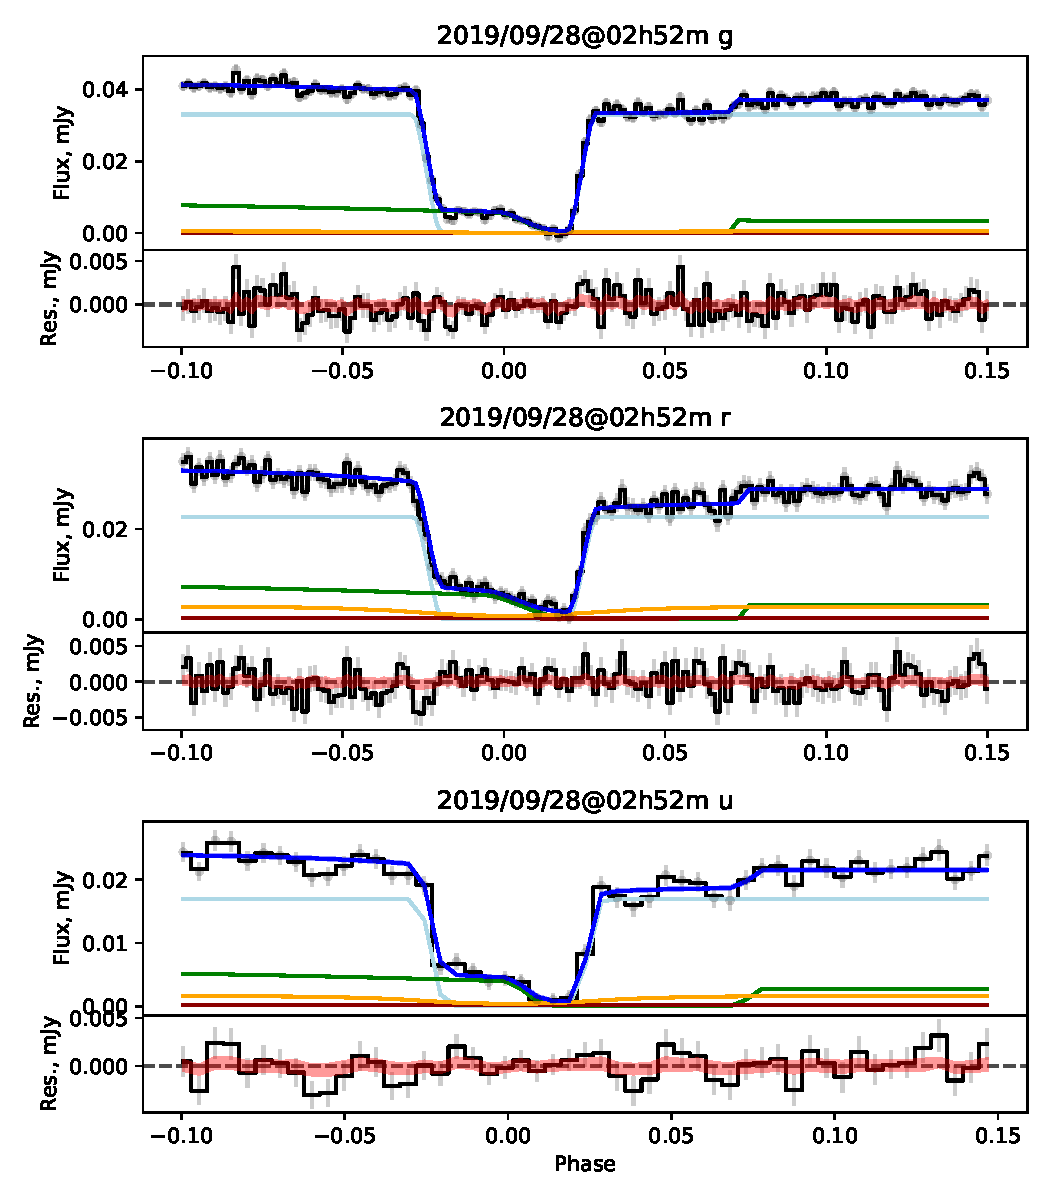
\includegraphics[width=\textwidth]{figures/results/three_cvs_with_weird_colours/ASASSN-17jf/ASASSN-17jf_1.pdf}
    \caption{ASASSN-17jf lightcurve models. {\it Top}:~{\bf grey points} are the observed flux, and note that the photometric system is the SDSS as per \S\ref{sect:observations:flux calibrating the lightcurve}; {\bf black line} is the observed flux, with the mean Gaussian process sample subtracted; the {\bf dark blue line} is the mean lightcurve model, and the {\bf blue band} is the standard deviation on this in the MCMC chain. The components of the model are also shown: the {\bf light blue line} is the white dwarf flux, {\bf green line} is the bright spot, {\bf orange line} is the disc, and the {\bf red line} is the donor. {\it Bottom}:~The residuals between the data and model are plotted as the {\bf black line}, with grey error bars. The Gaussian process 1-sigma region is shown as a {\bf red band}.}
    \label{fig:ASASSN-17jf all lightcurves}
\end{figure}
\begin{figure}
    \centering
    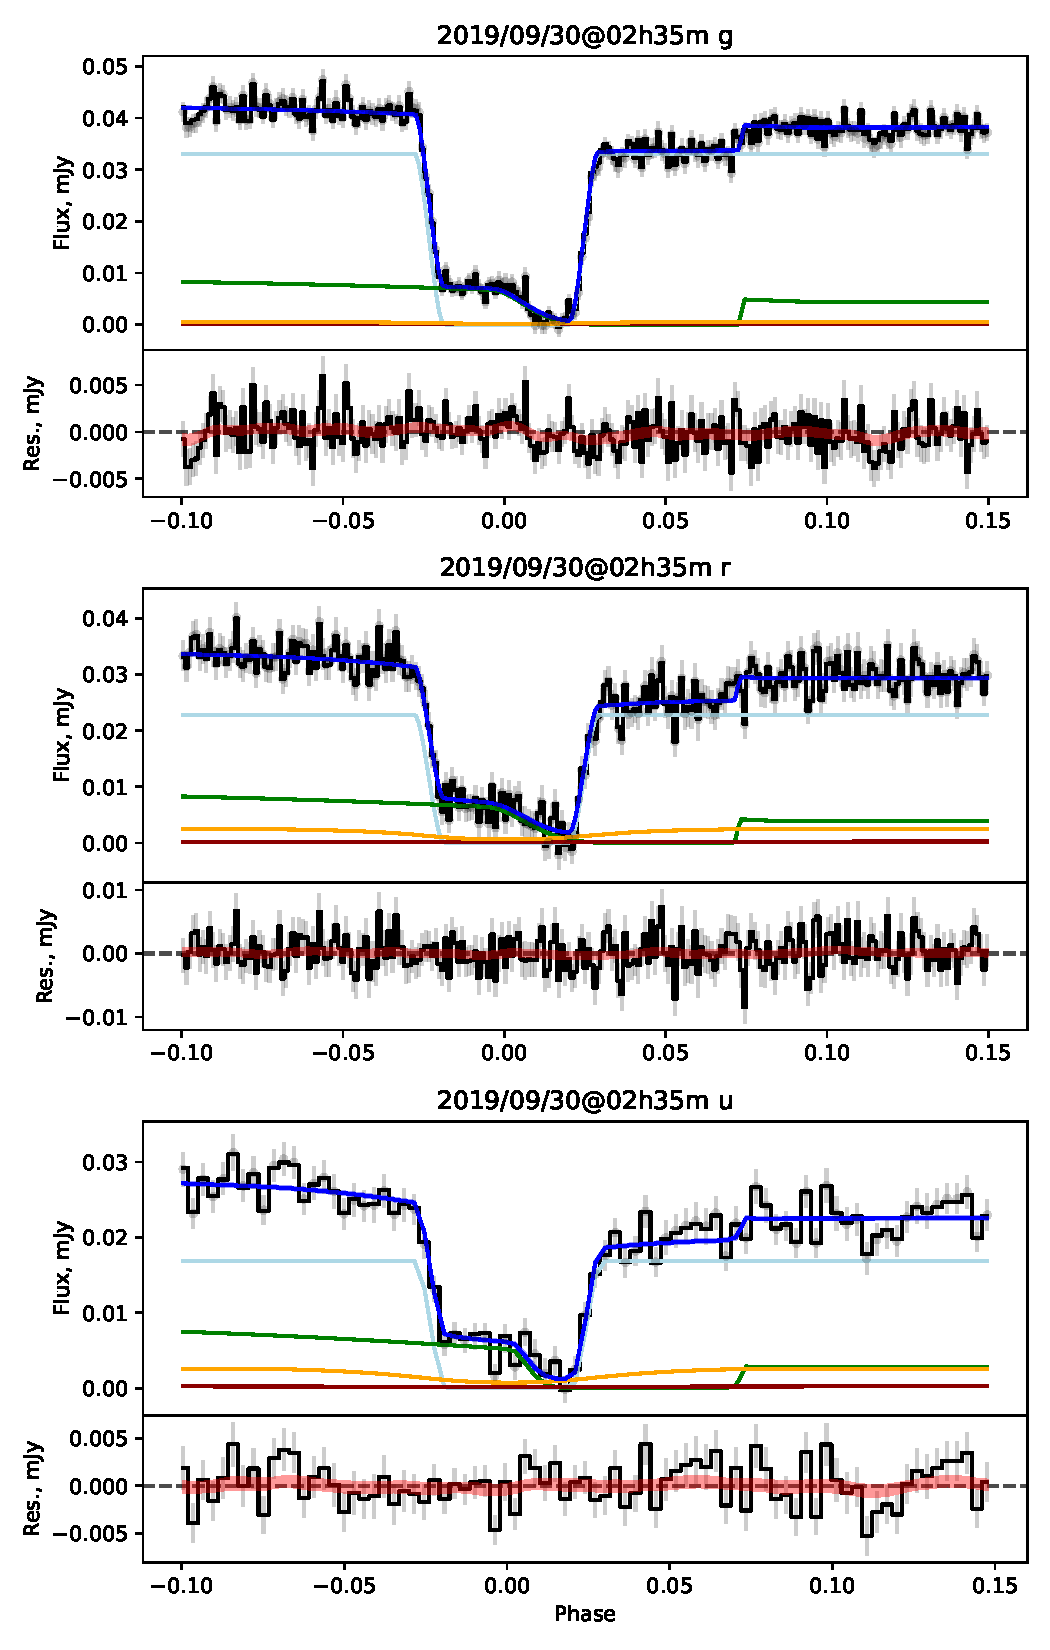
\includegraphics[width=\textwidth]{figures/results/three_cvs_with_weird_colours/ASASSN-17jf/ASASSN-17jf_2.pdf}
    \caption{ASASSN-17jf lightcurve models (cont.)}
    \label{fig:ASASSN-17jf all lightcurves cont 1}
\end{figure}
\begin{figure}
    \centering
    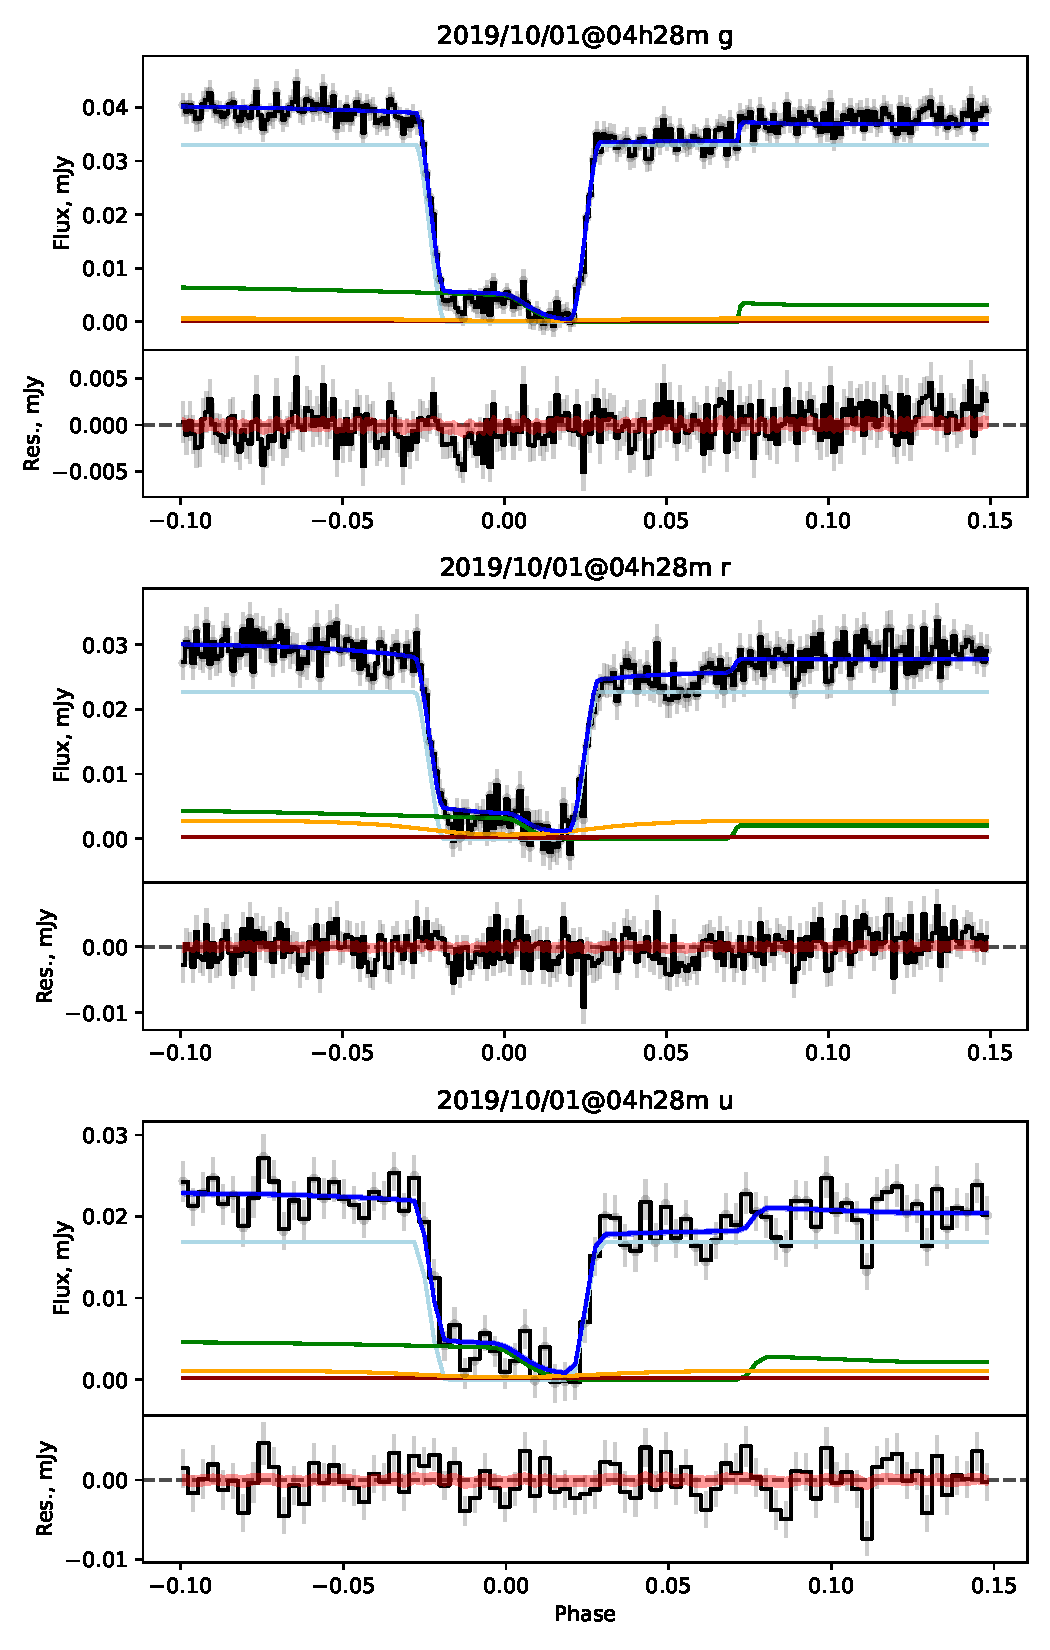
\includegraphics[width=\textwidth]{figures/results/three_cvs_with_weird_colours/ASASSN-17jf/ASASSN-17jf_3.pdf}
    \caption{ASASSN-17jf lightcurve models (cont.)}
    \label{fig:ASASSN-17jf all lightcurves cont 2}
\end{figure}



\begin{figure}
    \centering
    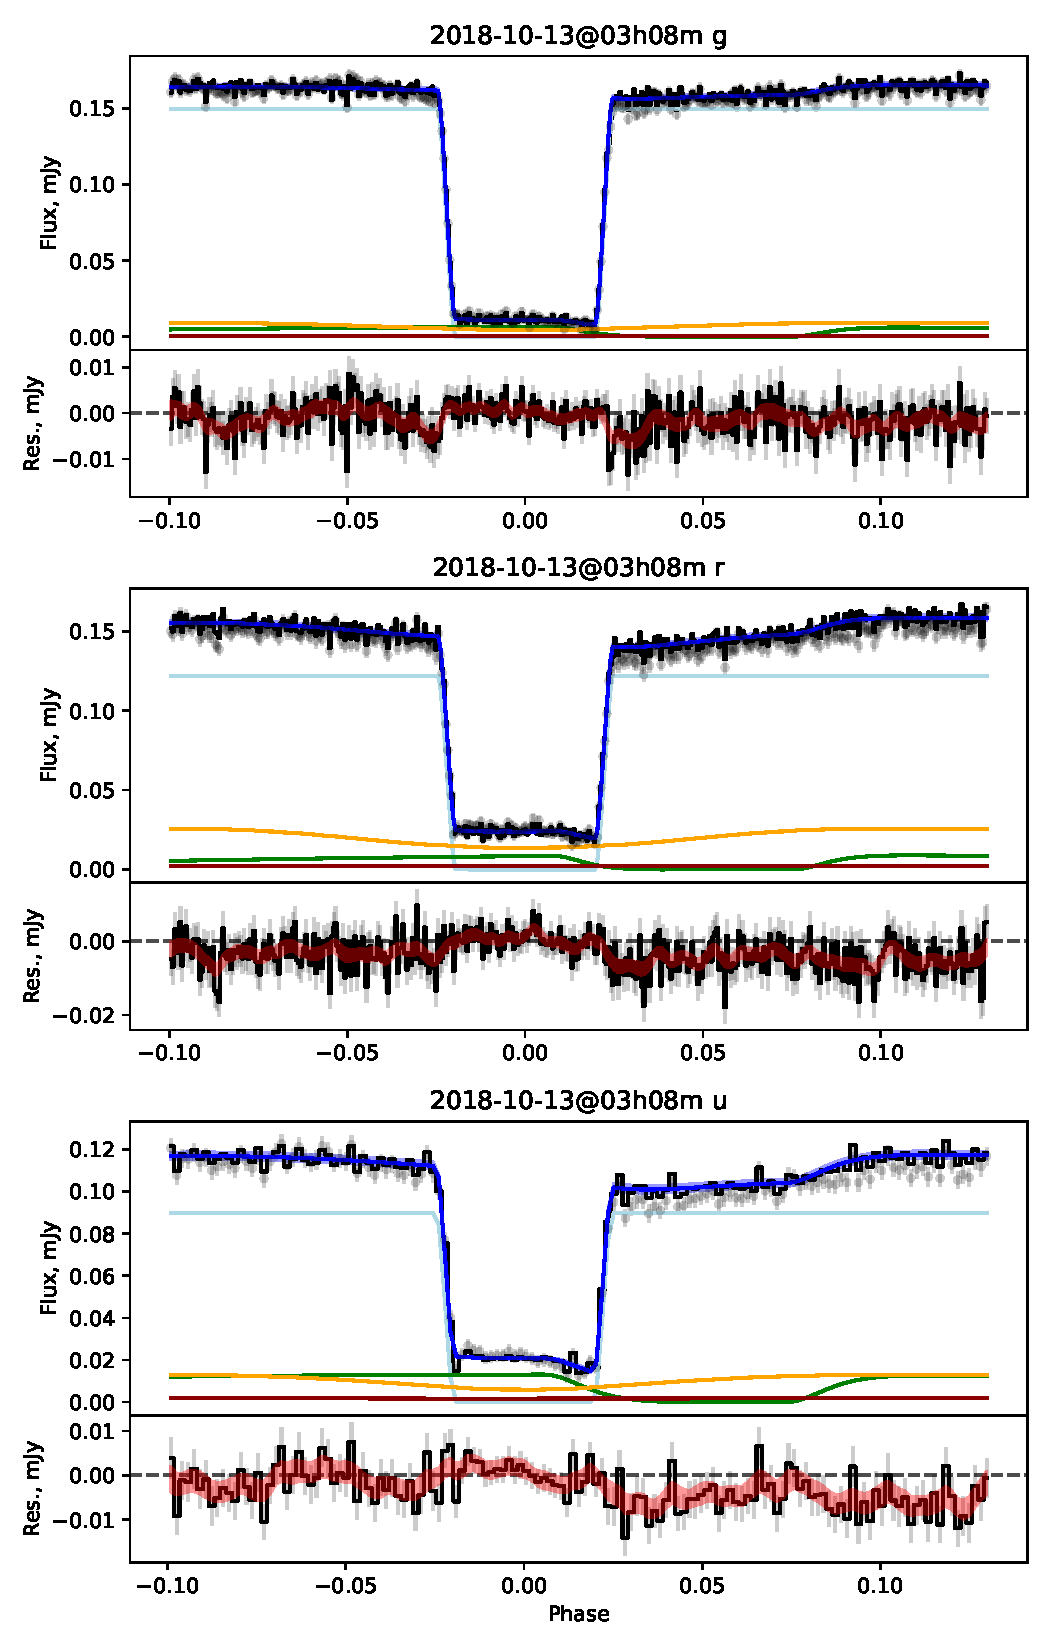
\includegraphics[width=\textwidth]{figures/results/three_cvs_with_weird_colours/ASASSN-16kr/ASASSN-16kr_1.pdf}
    \caption{ASASSN-16kr lightcurve models. Symbols are the same as Figure~\ref{fig:ASASSN-17jf all lightcurves}}
    \label{fig:ASASSN-16kr all lightcurves}
\end{figure}
\begin{figure}
    \centering
    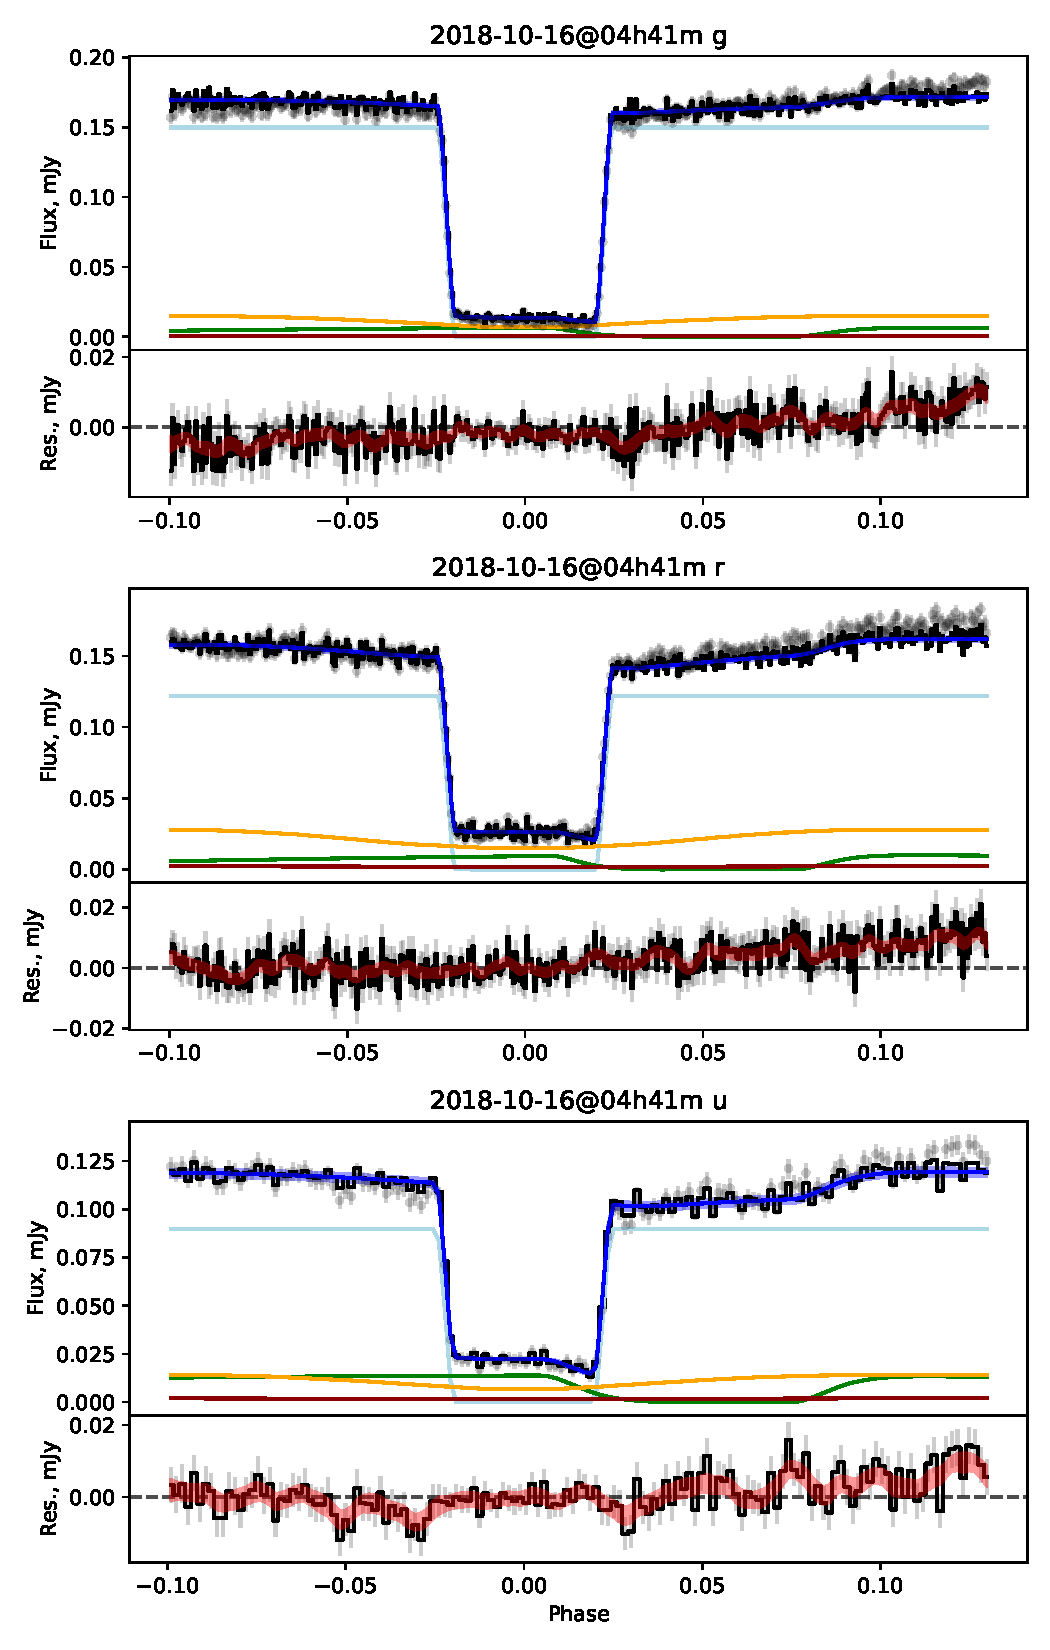
\includegraphics[width=\textwidth]{figures/results/three_cvs_with_weird_colours/ASASSN-16kr/ASASSN-16kr_2.pdf}
    \caption{ASASSN-16kr lightcurve models (cont.)}
    \label{fig:ASASSN-16kr all lightcurves cont 1}
\end{figure}
\begin{figure}
    \centering
    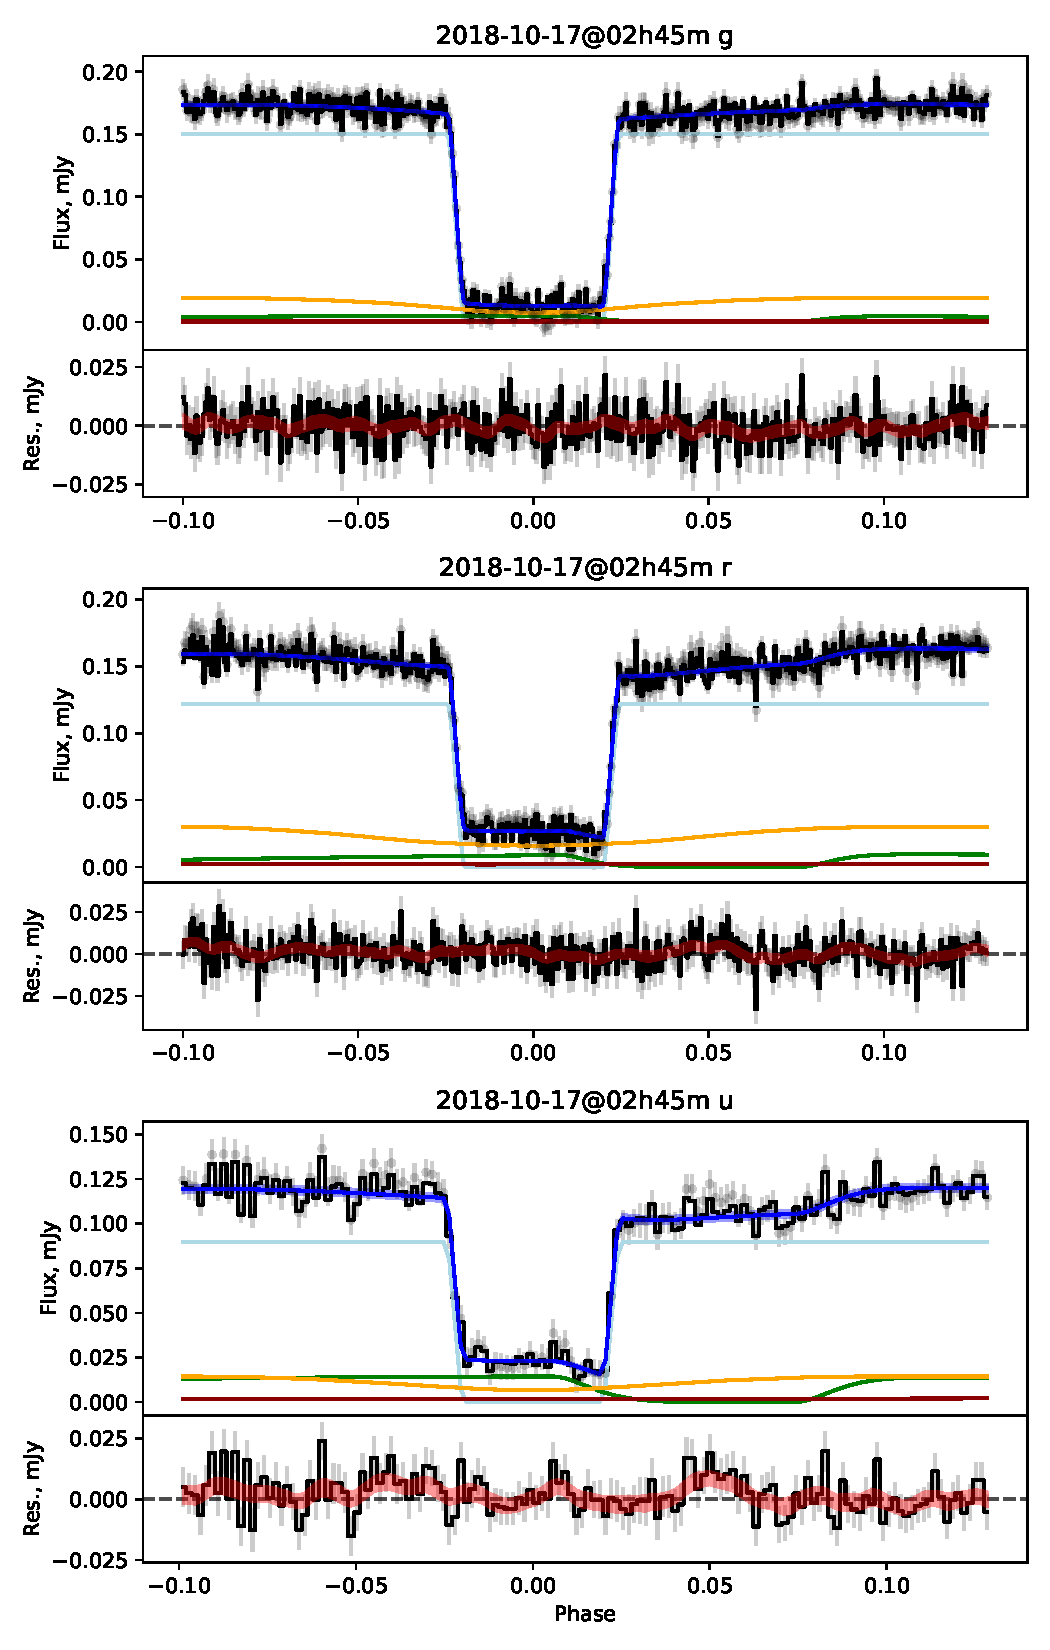
\includegraphics[width=\textwidth]{figures/results/three_cvs_with_weird_colours/ASASSN-16kr/ASASSN-16kr_3.pdf}
    \caption{ASASSN-16kr lightcurve models (cont.)}
    \label{fig:ASASSN-16kr all lightcurves cont 2}
\end{figure}
\begin{figure}
    \centering
    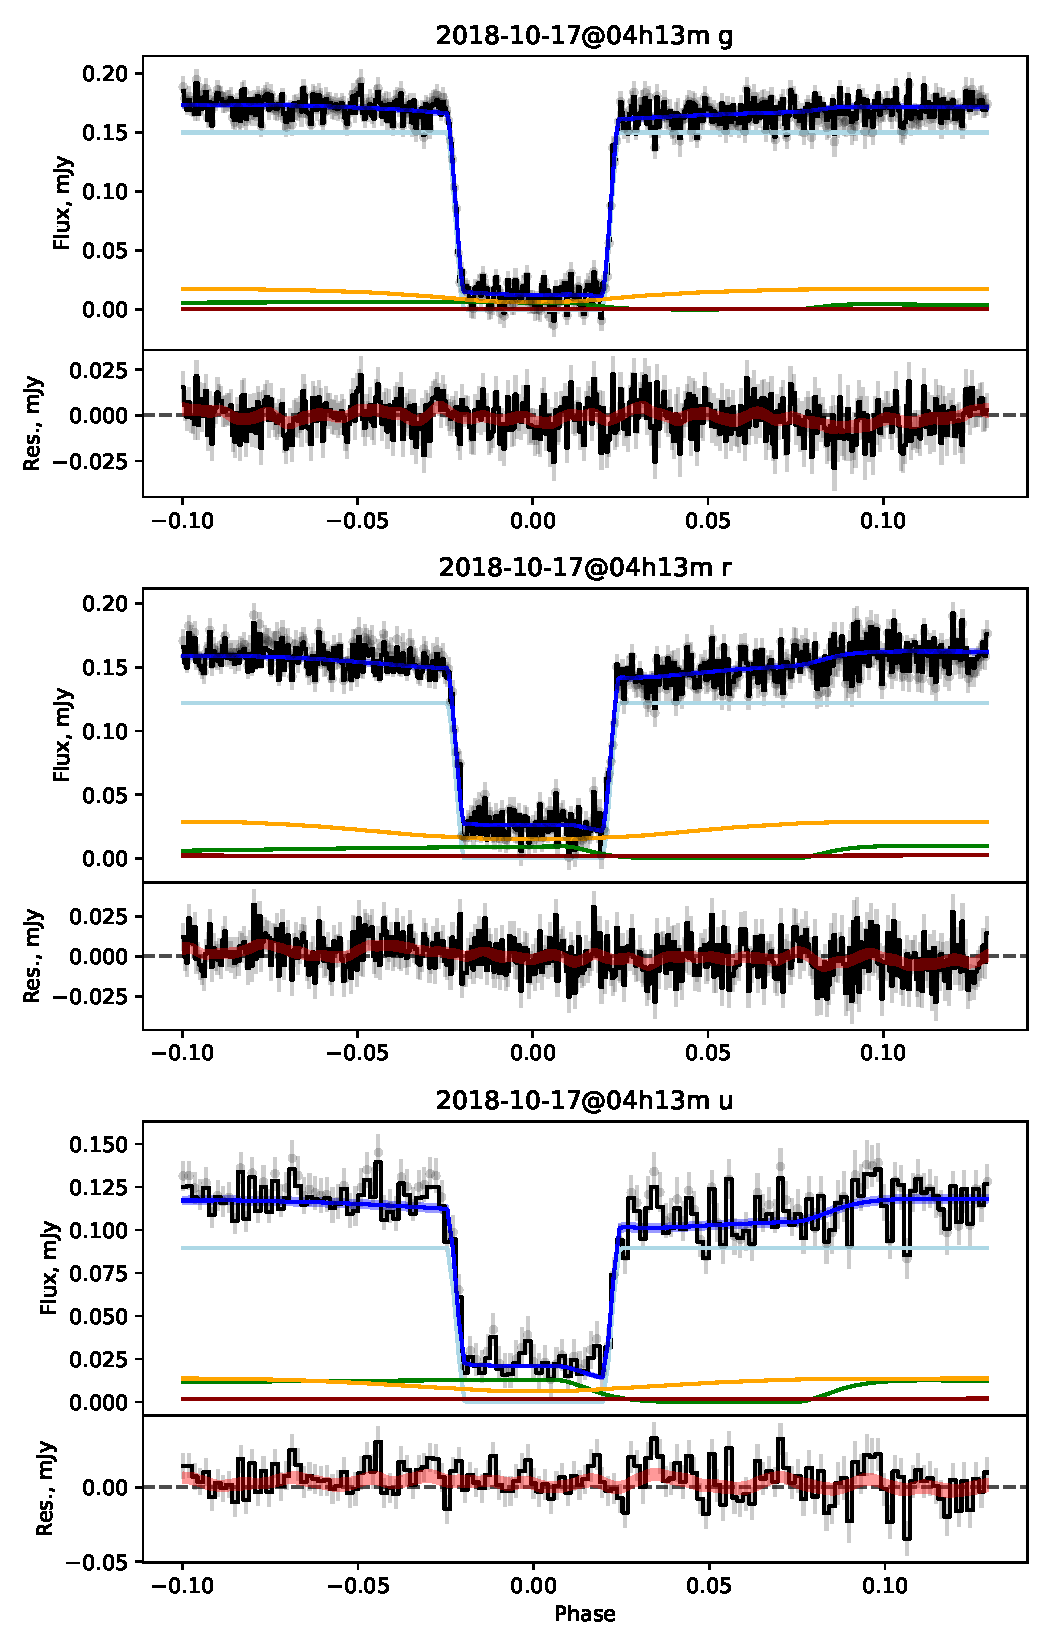
\includegraphics[width=\textwidth]{figures/results/three_cvs_with_weird_colours/ASASSN-16kr/ASASSN-16kr_4.pdf}
    \caption{ASASSN-16kr lightcurve models (cont.)}
    \label{fig:ASASSN-16kr all lightcurves cont 3}
\end{figure}
\begin{figure}
    \centering
    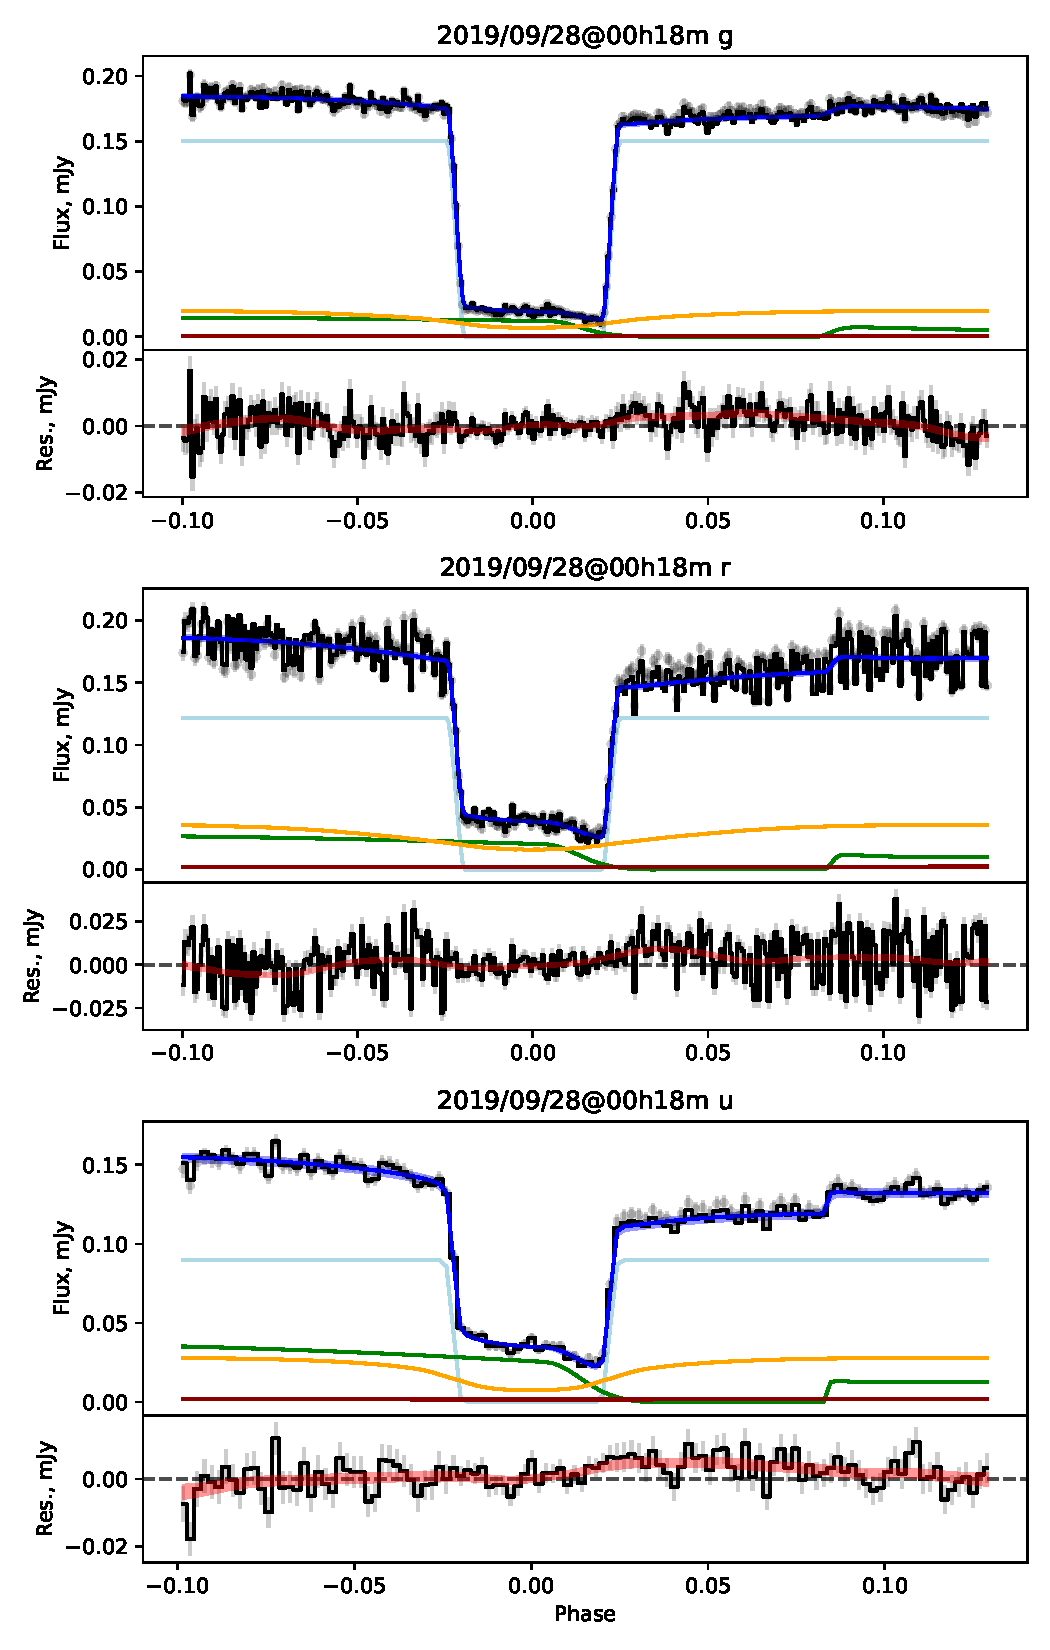
\includegraphics[width=\textwidth]{figures/results/three_cvs_with_weird_colours/ASASSN-16kr/ASASSN-16kr_5.pdf}
    \caption{ASASSN-16kr lightcurve models (cont.)}
    \label{fig:ASASSN-16kr all lightcurves cont 4}
\end{figure}
\begin{figure}
    \centering
    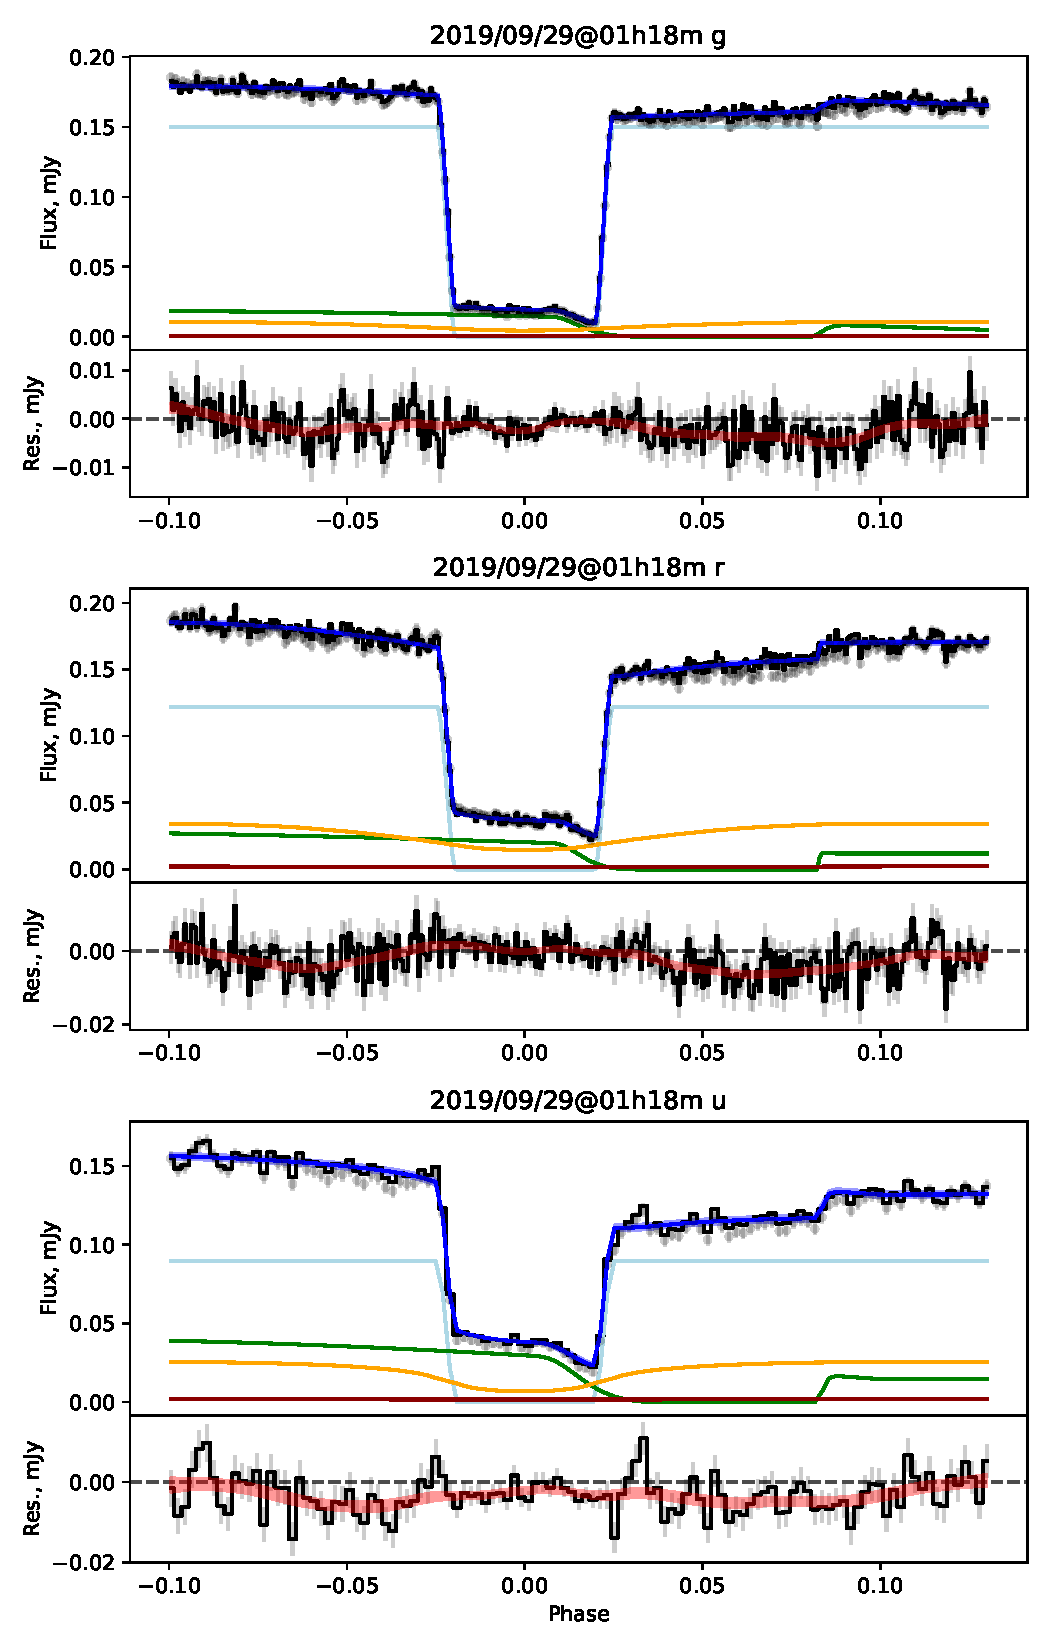
\includegraphics[width=\textwidth]{figures/results/three_cvs_with_weird_colours/ASASSN-16kr/ASASSN-16kr_6.pdf}
    \caption{ASASSN-16kr lightcurve models (cont.)}
    \label{fig:ASASSN-16kr all lightcurves cont 5}
\end{figure}
\begin{figure}
    \centering
    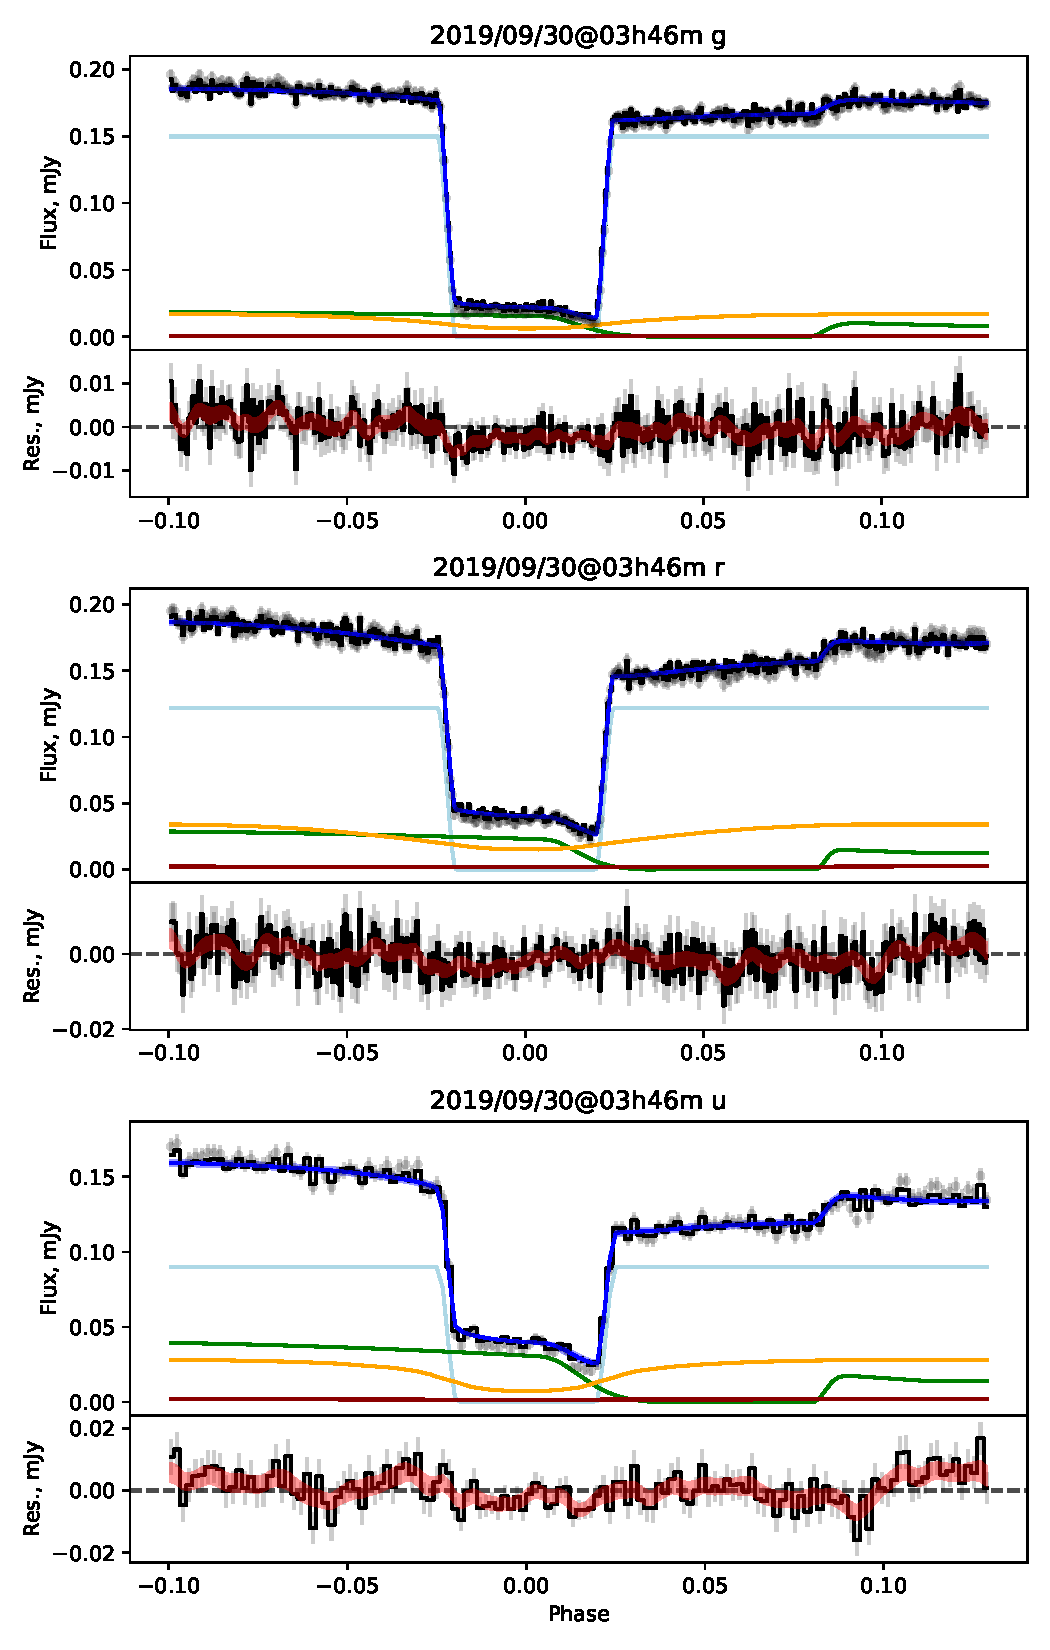
\includegraphics[width=\textwidth]{figures/results/three_cvs_with_weird_colours/ASASSN-16kr/ASASSN-16kr_7.pdf}
    \caption{ASASSN-16kr lightcurve models (cont.)}
    \label{fig:ASASSN-16kr all lightcurves cont 6}
\end{figure}



\begin{figure}
    \centering
    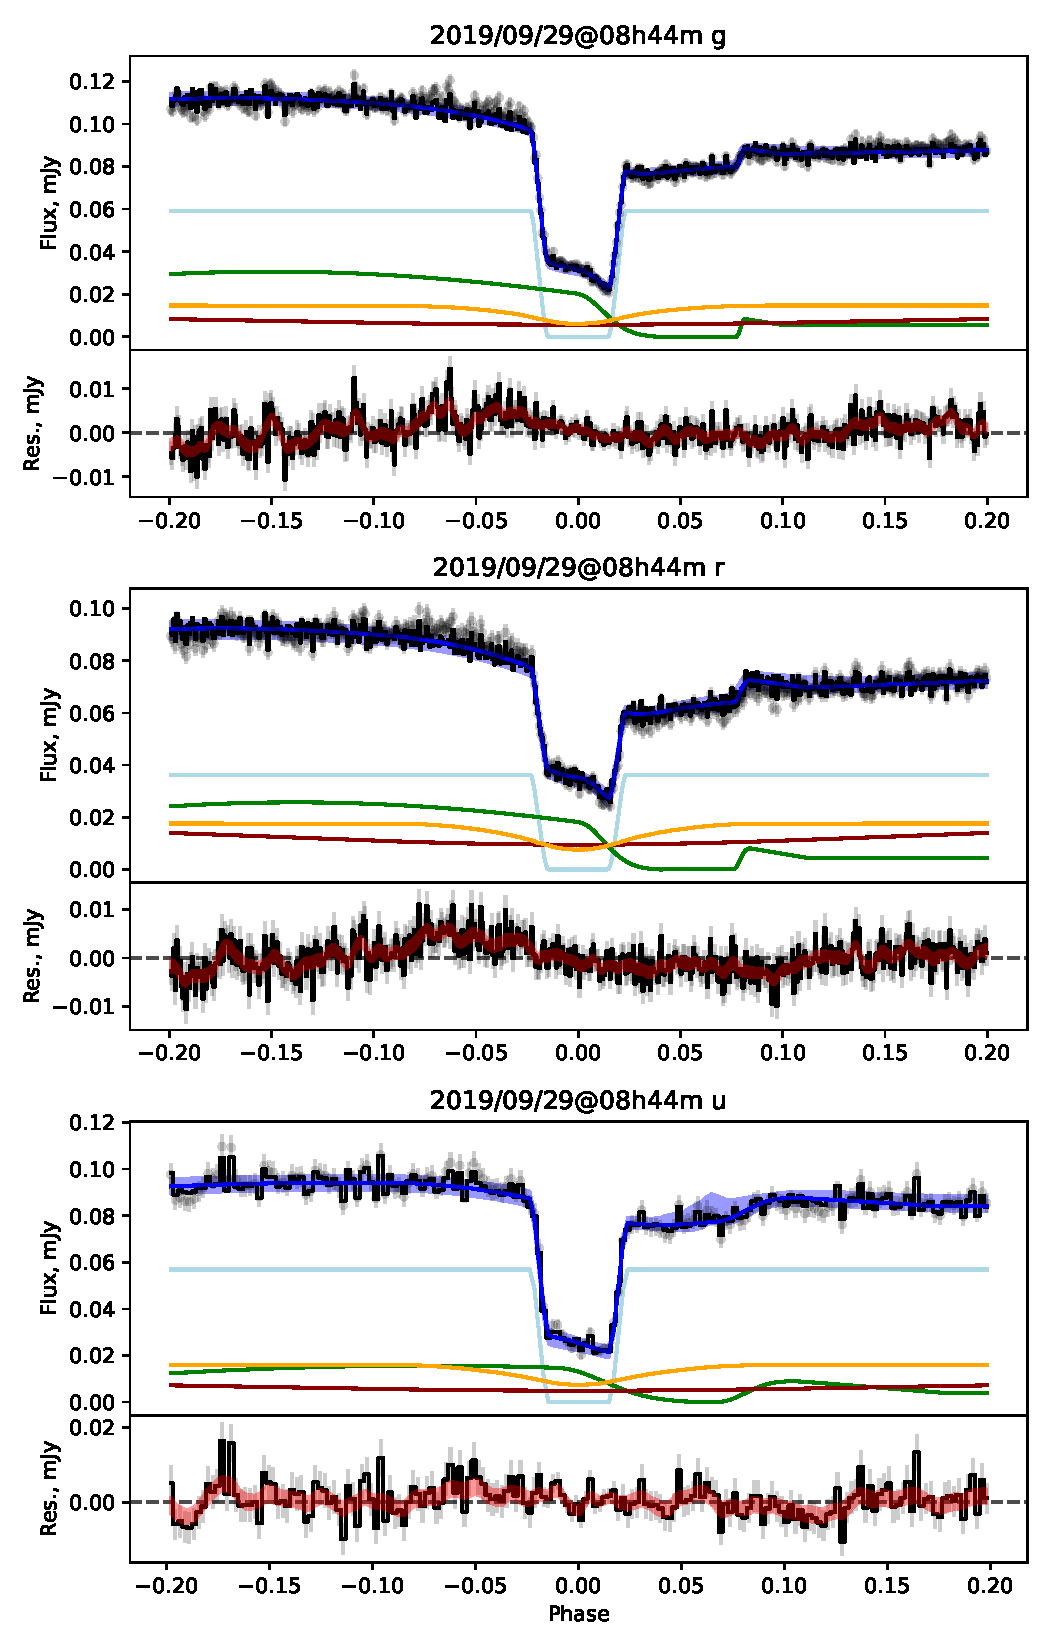
\includegraphics[width=\textwidth]{figures/results/three_cvs_with_weird_colours/SSS111126/SSS111126_1.pdf}
    \caption{SSSJ0522-3505 lightcurve models. Symbols are the same as Figure~\ref{fig:ASASSN-17jf all lightcurves}}
    \label{fig:SSSJ0522-3505 all lightcurves}
\end{figure}
\begin{figure}
    \centering
    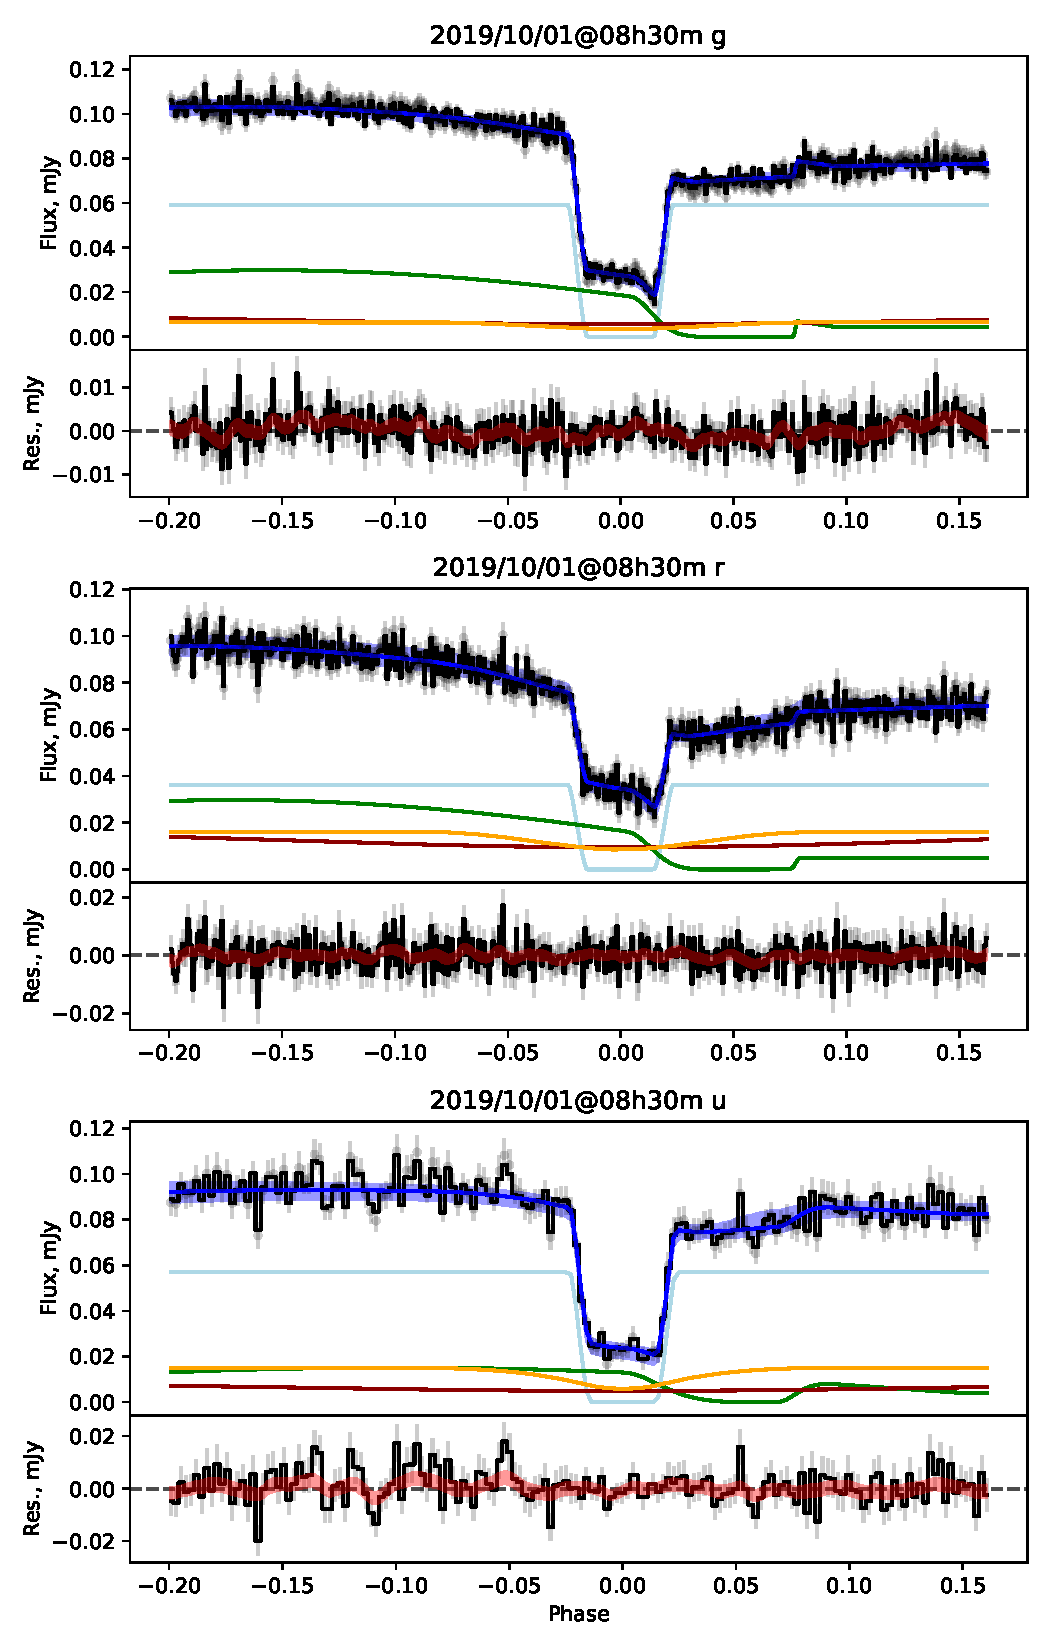
\includegraphics[width=\textwidth]{figures/results/three_cvs_with_weird_colours/SSS111126/SSS111126_2.pdf}
    \caption{SSSJ0522-3505 lightcurve models (cont.)}
    \label{fig:SSSJ0522-3505 all lightcurves cont 1}
\end{figure}
\begin{figure}
    \centering
    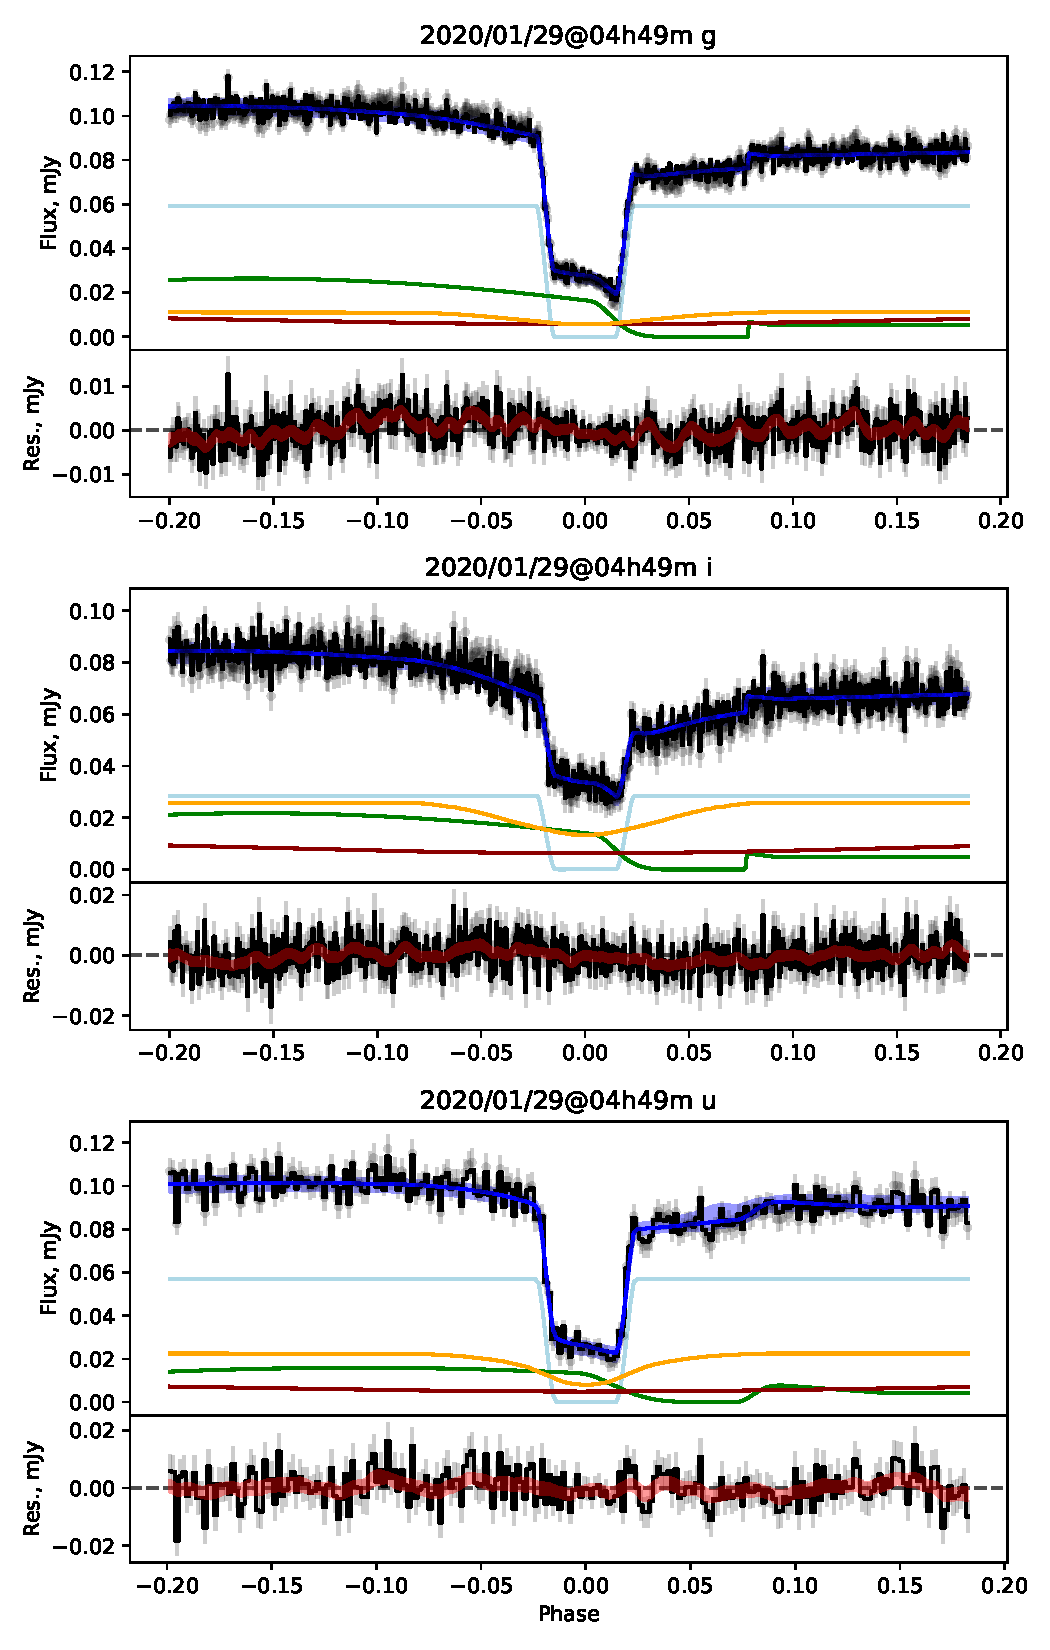
\includegraphics[width=\textwidth]{figures/results/three_cvs_with_weird_colours/SSS111126/SSS111126_3.pdf}
    \caption{SSSJ0522-3505 lightcurve models (cont.)}
    \label{fig:SSSJ0522-3505 all lightcurves cont 2}
\end{figure}



\begin{figure}
    \centering
    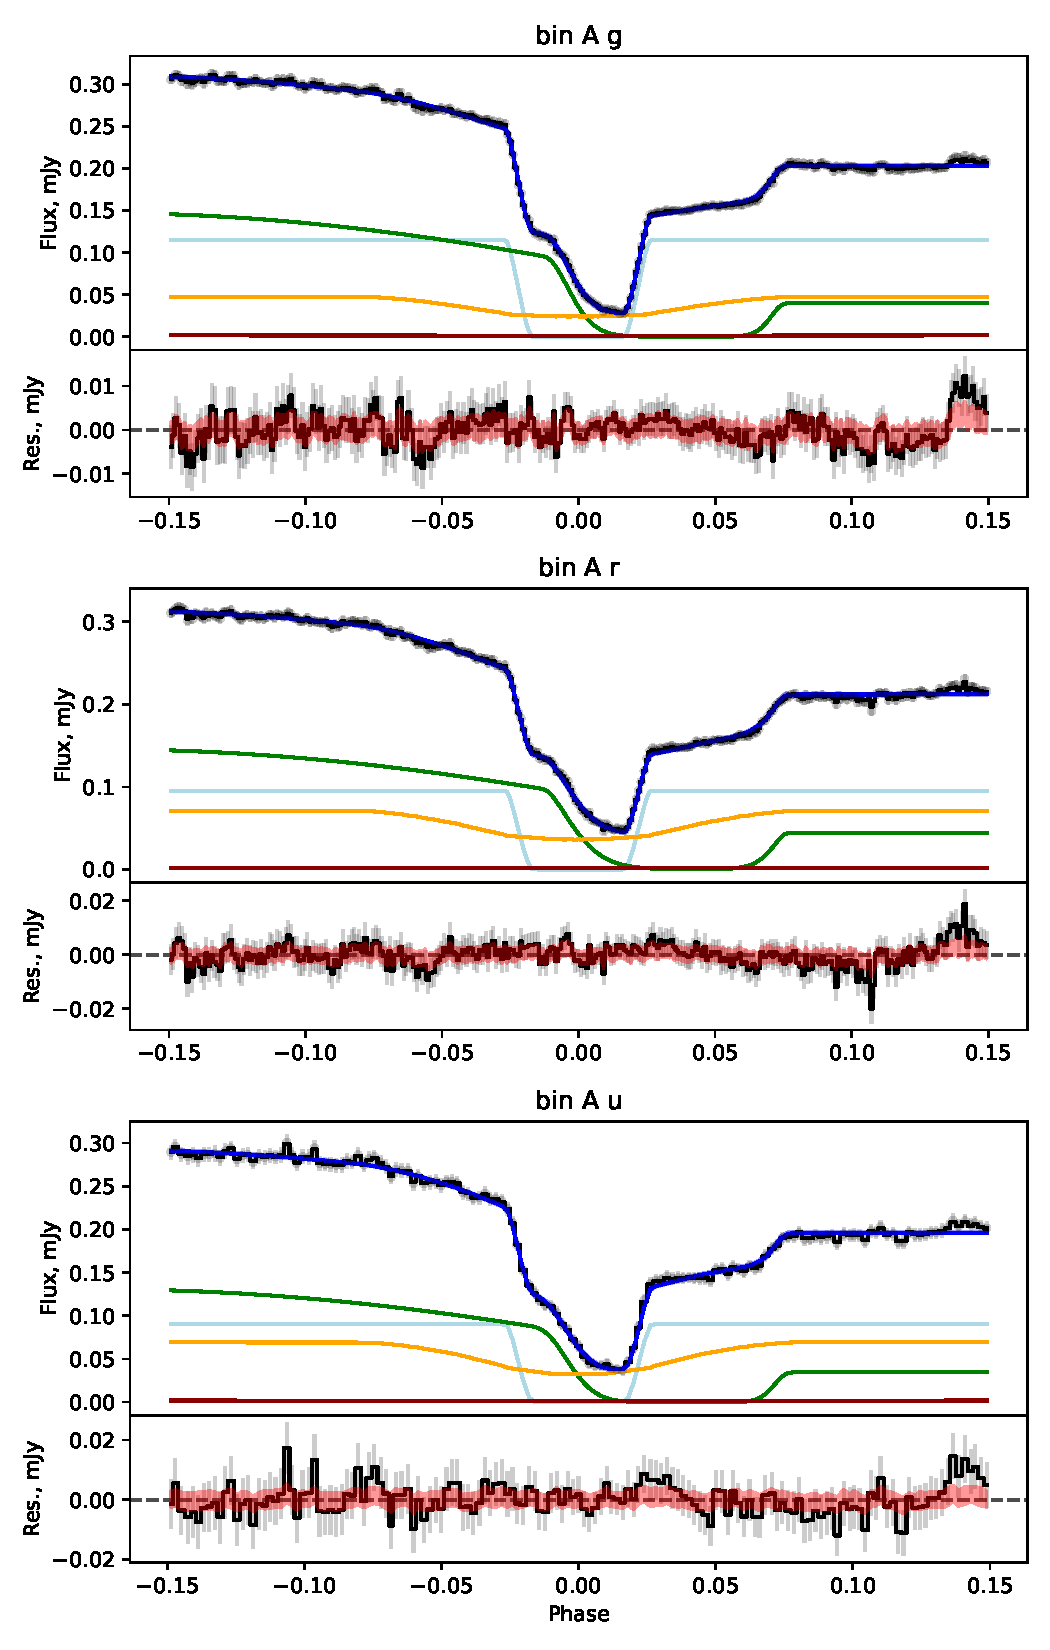
\includegraphics[width=\textwidth]{figures/results/ASASSN-14hq/ASASSN-14hq_1.pdf}
    \caption{ASASSN-14hq lightcurve models. Symbols are the same as Figure~\ref{fig:ASASSN-17jf all lightcurves}}
    \label{fig:ASASSN-14hq all lightcurves}
\end{figure}
\begin{figure}
    \centering
    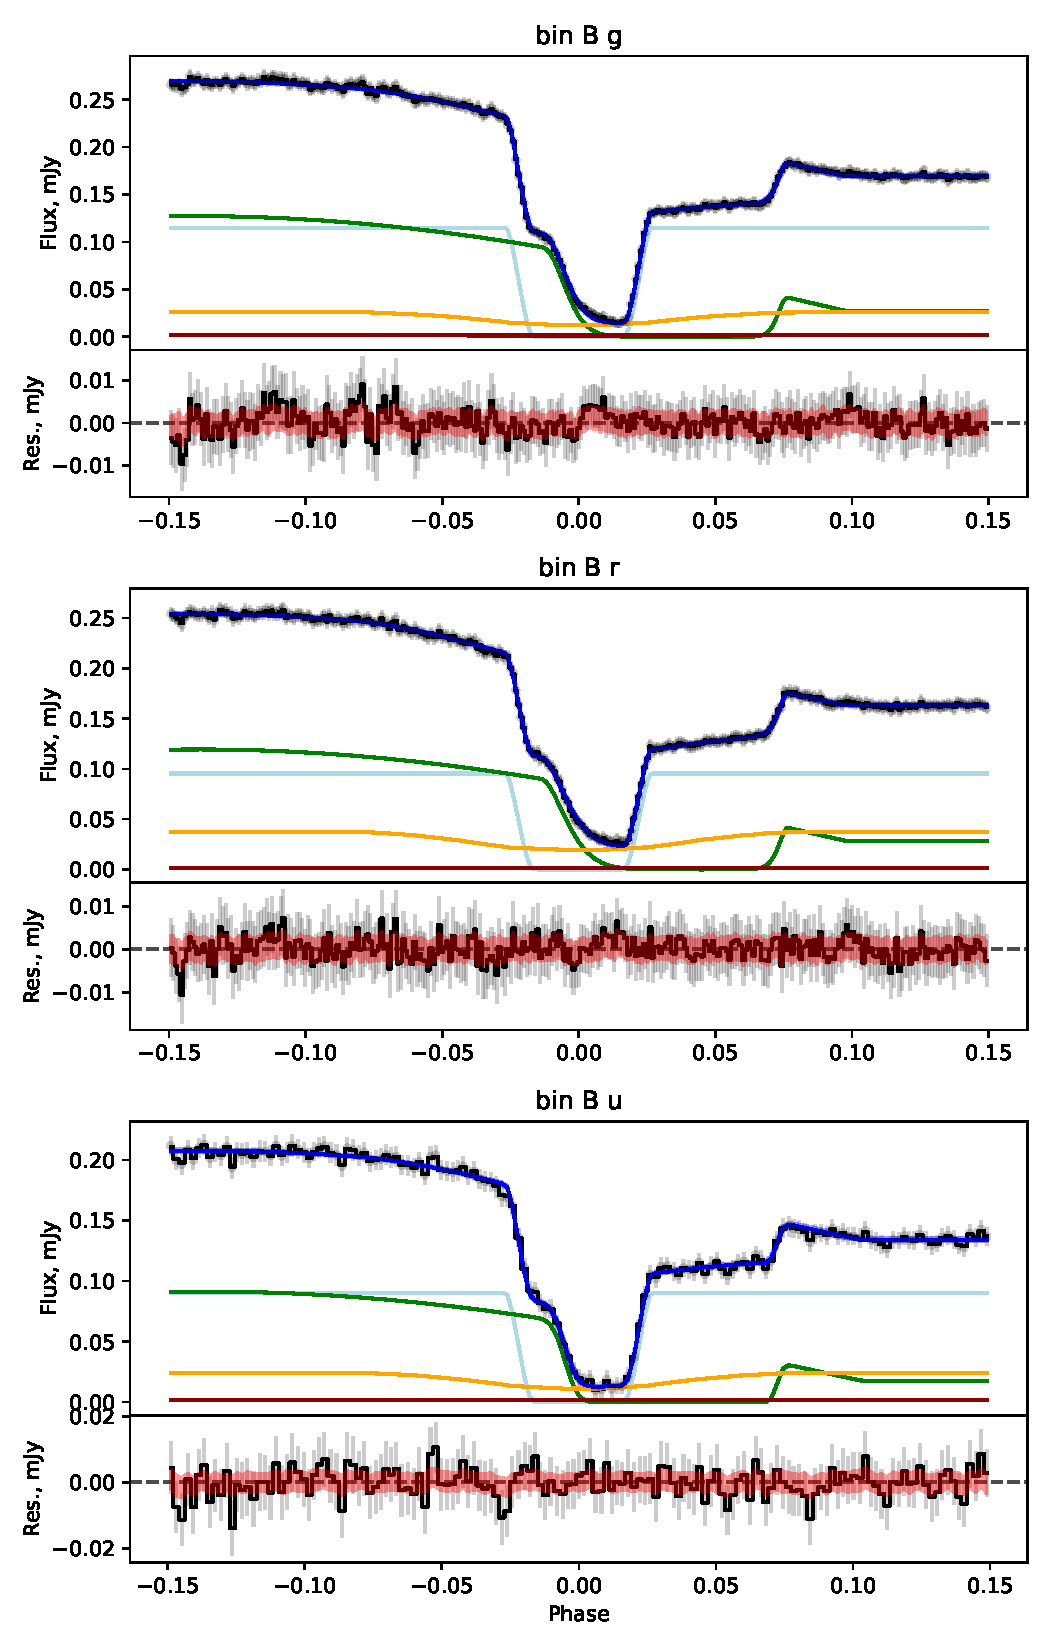
\includegraphics[width=\textwidth]{figures/results/ASASSN-14hq/ASASSN-14hq_2.pdf}
    \caption{ASASSN-14hq lightcurve models (cont.)}
    \label{fig:ASASSN-14hq all lightcurves cont}
\end{figure}



\begin{figure}
    \centering
    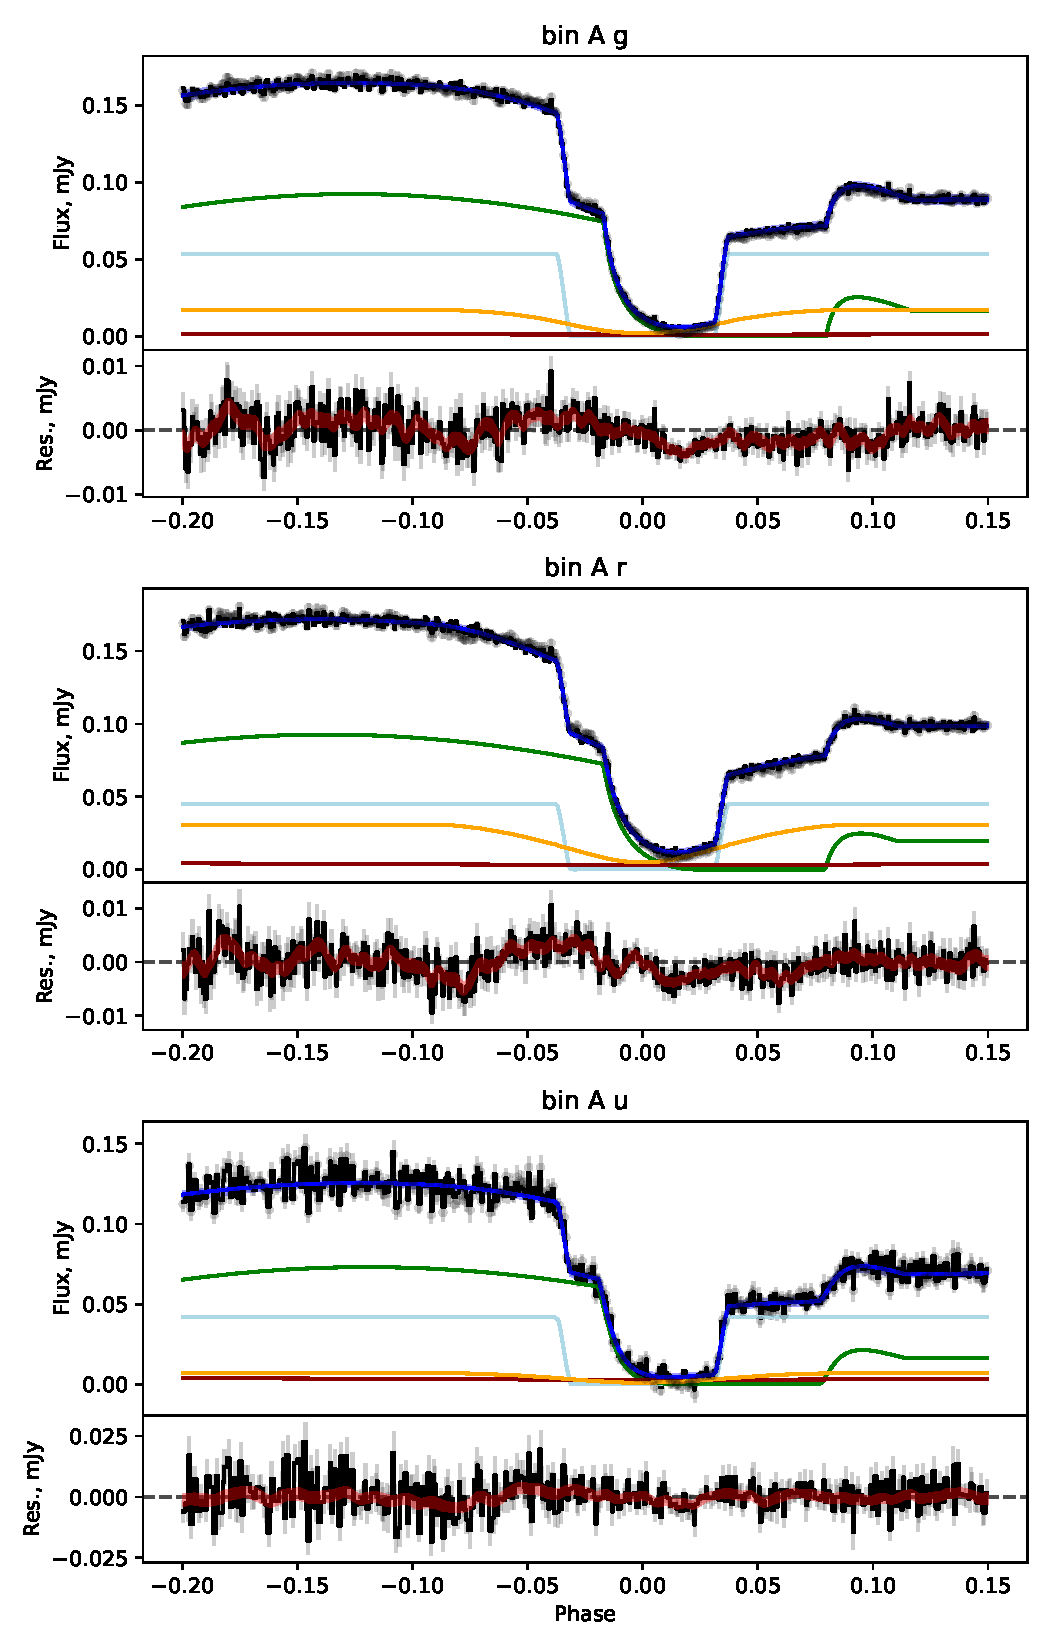
\includegraphics[width=\textwidth]{figures/results/ASASSN-14kb/ASASSN-14kb_1.pdf}
    \caption{ASASSN-14kb lightcurve models. Symbols are the same as Figure~\ref{fig:ASASSN-17jf all lightcurves}}
    \label{fig:ASASSN-14kb all lightcurves}
\end{figure}



\begin{figure}
    \centering
    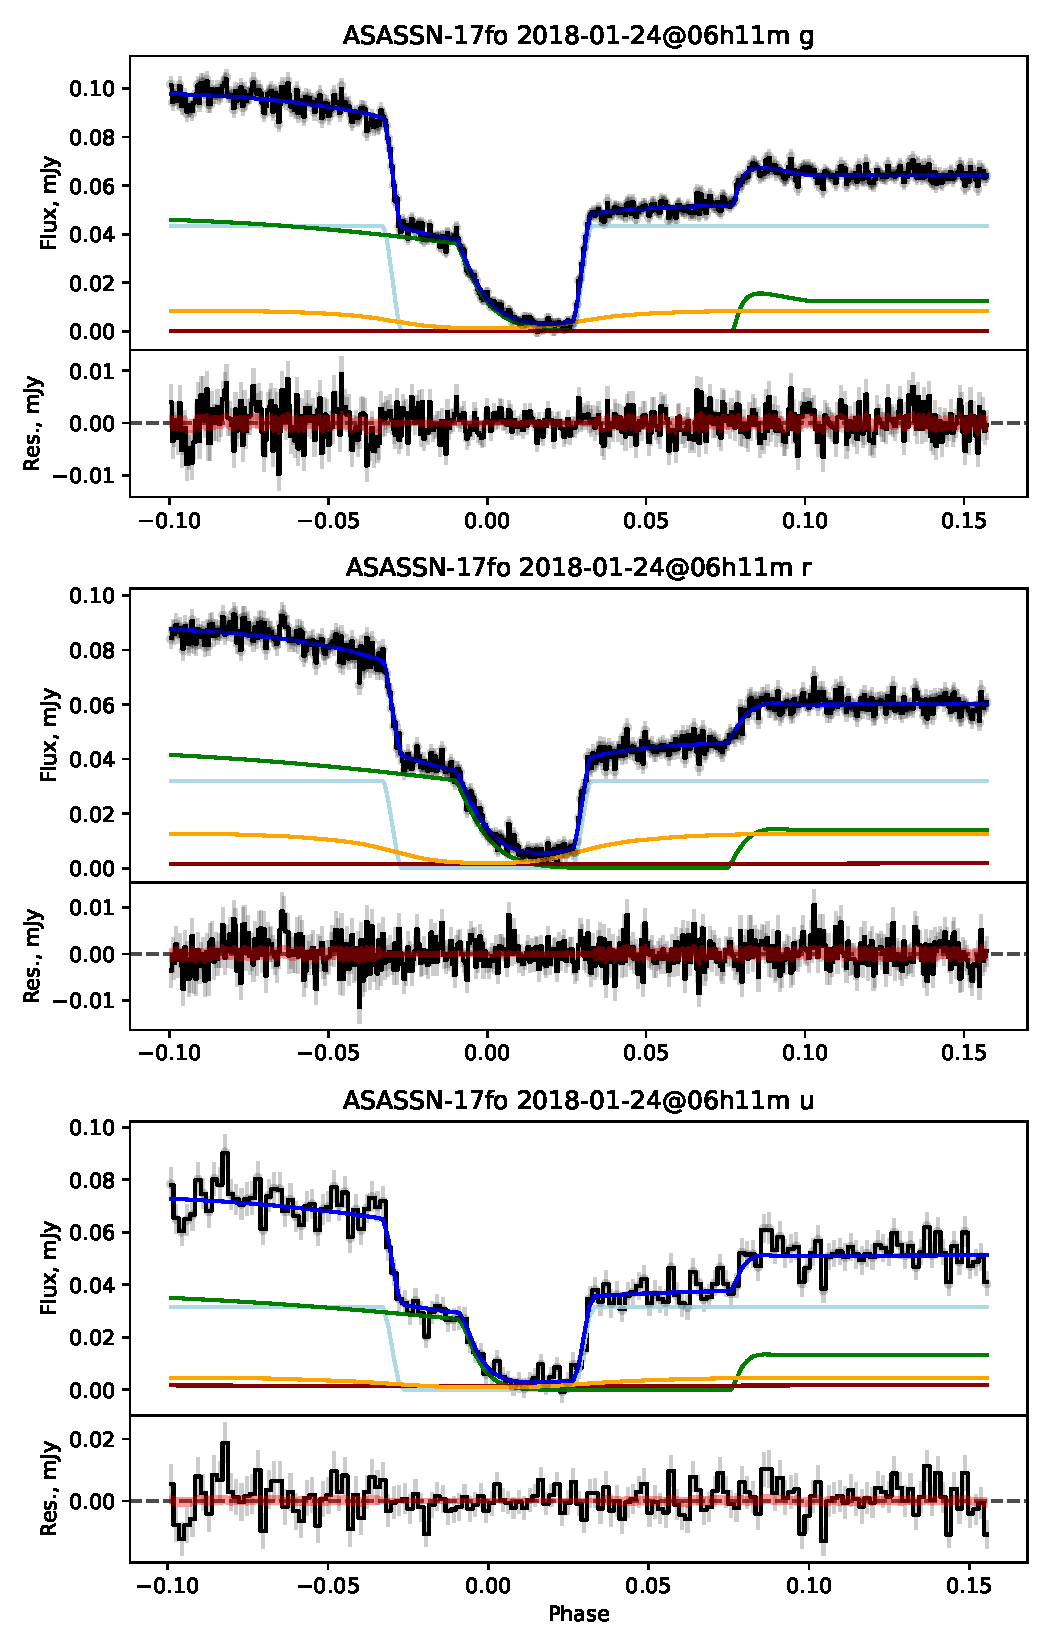
\includegraphics[width=\textwidth]{figures/results/ASASSN-17fo/ASASSN-17fo_1.pdf}
    \caption{ASASSN-17fo lightcurve models. Symbols are the same as Figure~\ref{fig:ASASSN-17jf all lightcurves}}
    \label{fig:ASASSN-17fo all lightcurves}
\end{figure}
\begin{figure}
    \centering
    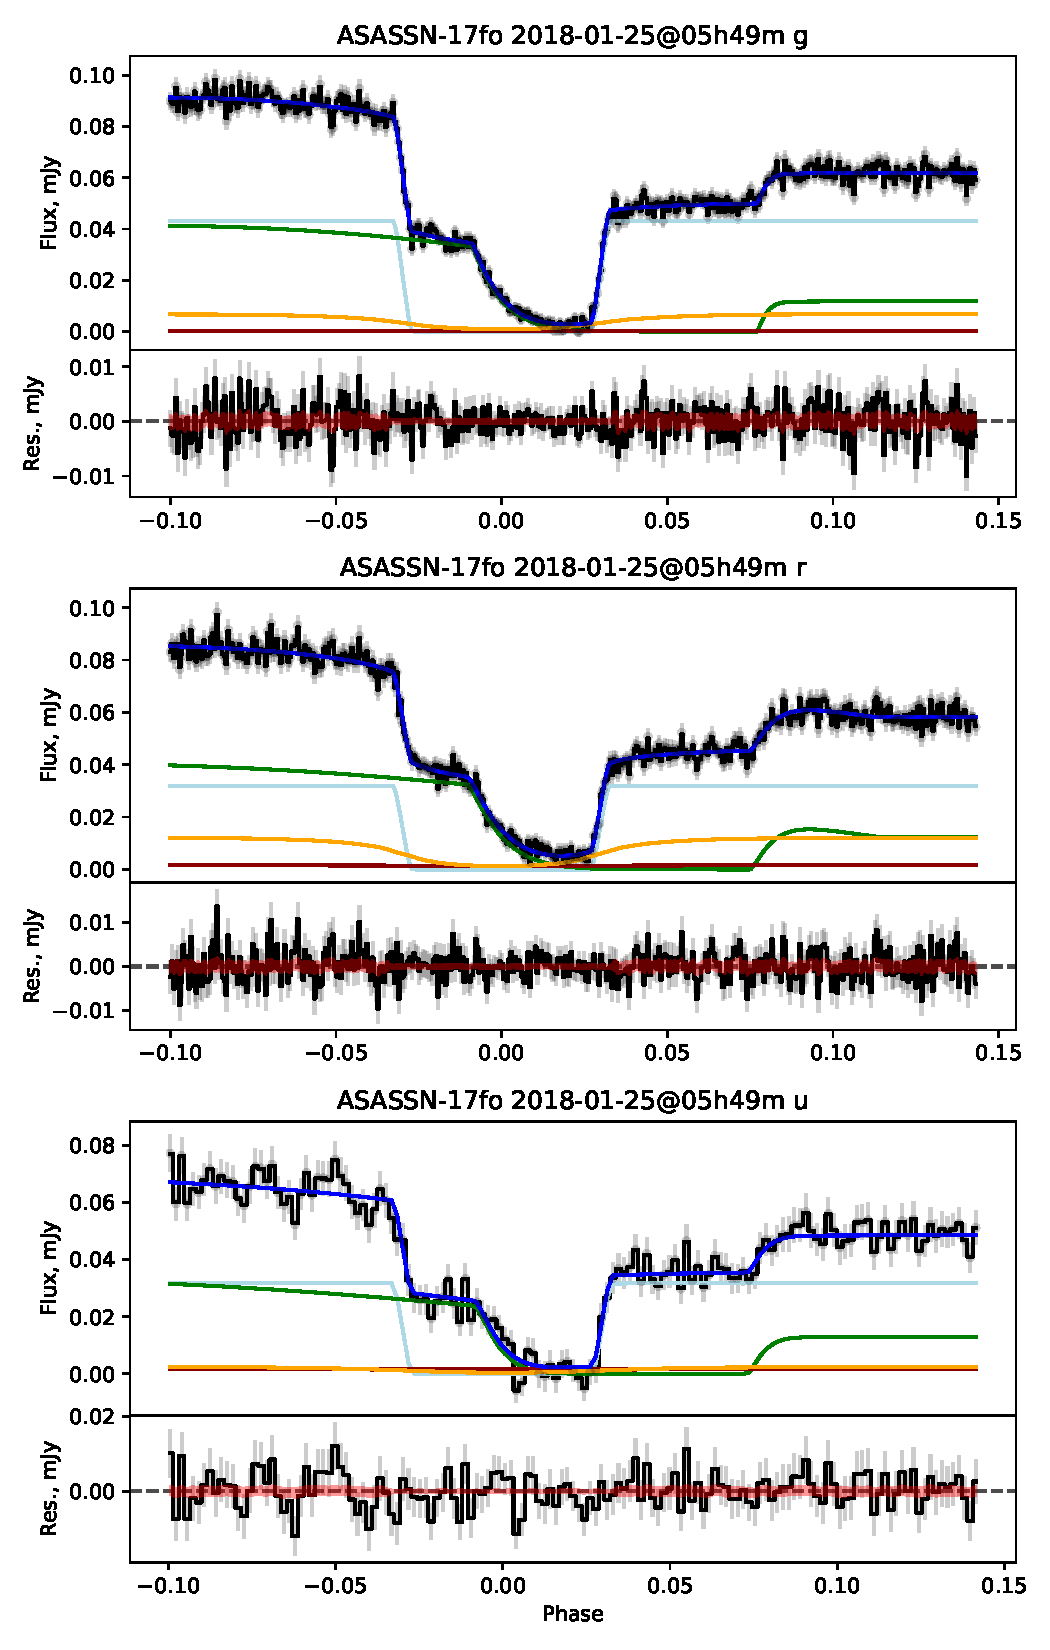
\includegraphics[width=\textwidth]{figures/results/ASASSN-17fo/ASASSN-17fo_2.pdf}
    \caption{ASASSN-17fo lightcurve models (cont.)}
    \label{fig:ASASSN-17fo all lightcurves cont 1}
\end{figure}
\begin{figure}
    \centering
    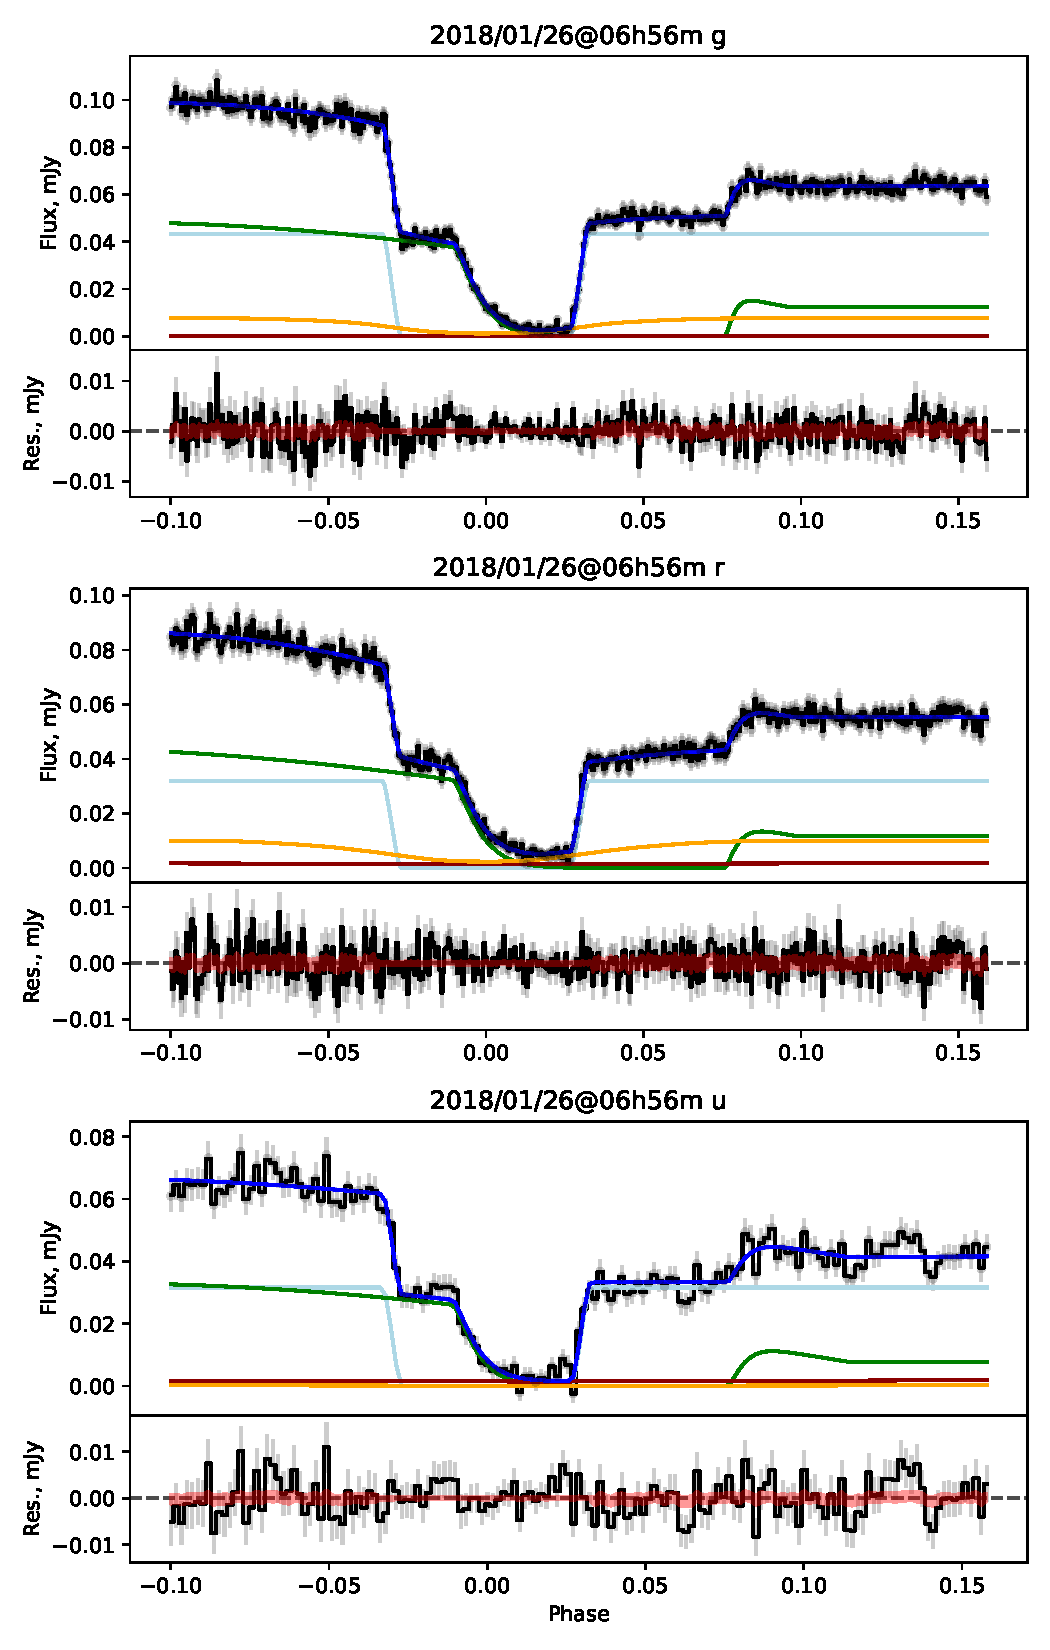
\includegraphics[width=\textwidth]{figures/results/ASASSN-17fo/ASASSN-17fo_3.pdf}
    \caption{ASASSN-17fo lightcurve models (cont.)}
    \label{fig:ASASSN-17fo all lightcurves cont 2}
\end{figure}



\begin{figure}
    \centering
    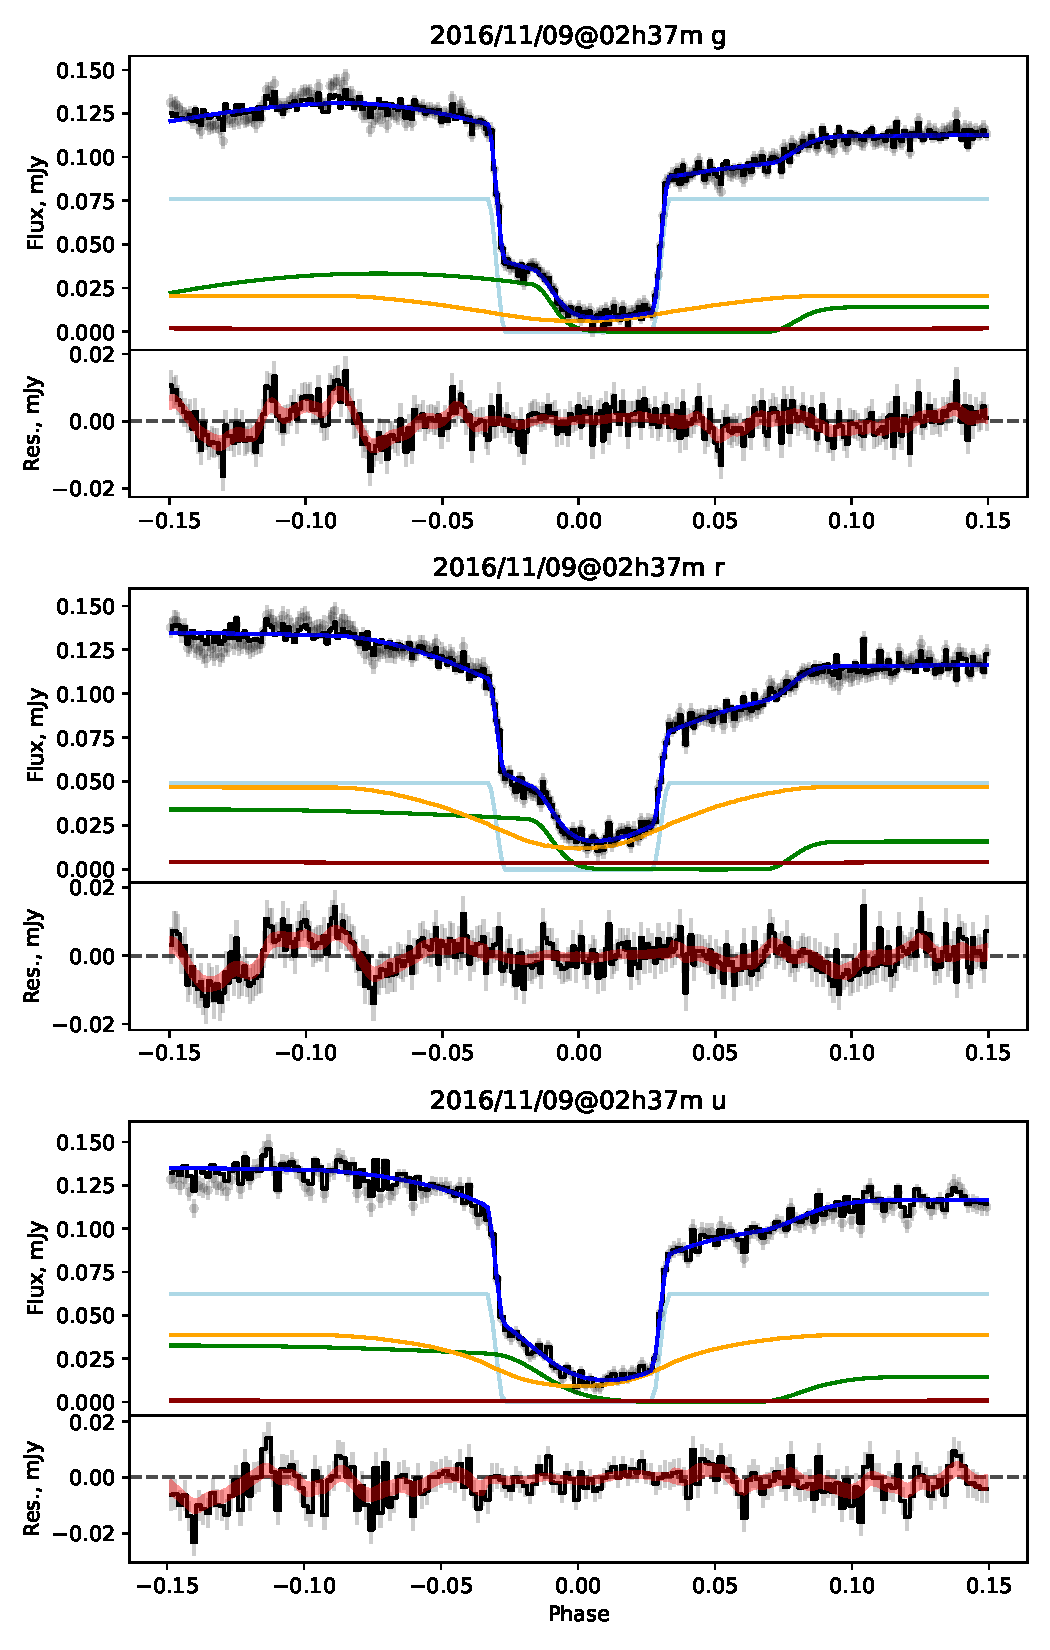
\includegraphics[width=\textwidth]{figures/results/AYFor/AYFor_1.pdf}
    \caption{AY For lightcurve models. Symbols are the same as Figure~\ref{fig:ASASSN-17jf all lightcurves}}
    \label{fig:AYFor all lightcurves}
\end{figure}
\begin{figure}
    \centering
    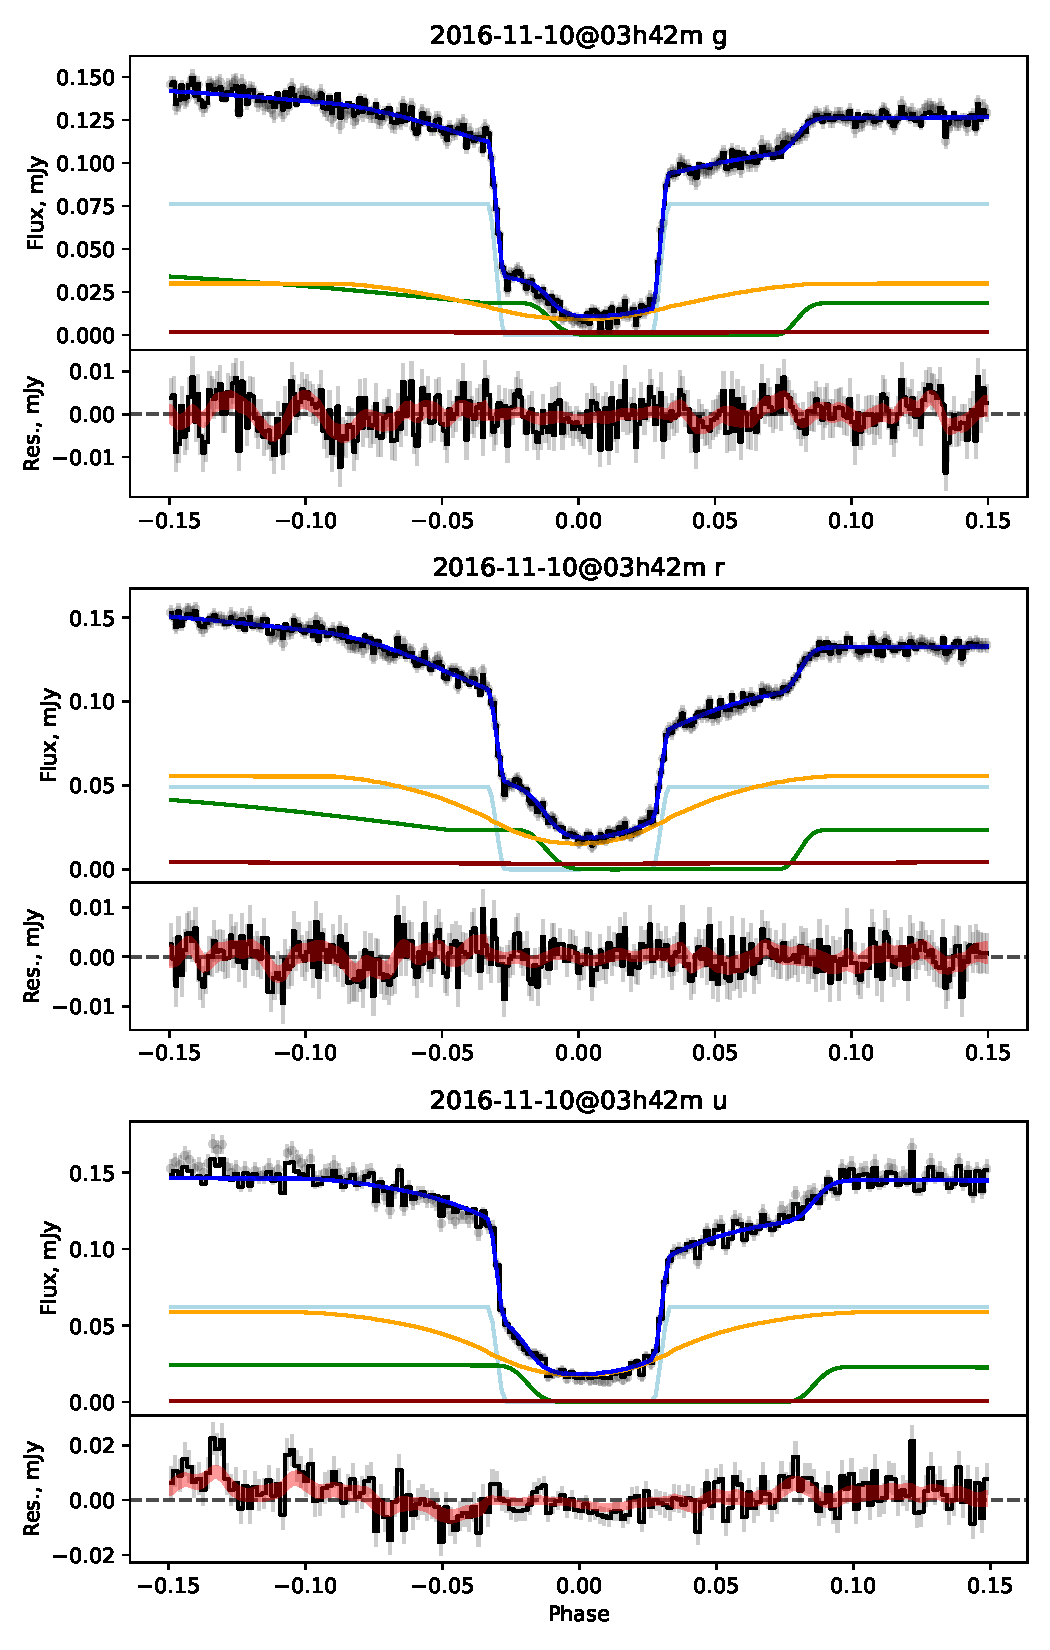
\includegraphics[width=\textwidth]{figures/results/AYFor/AYFor_2.pdf}
    \caption{AY For lightcurve models (cont.)}
    \label{fig:AYFor all lightcurves cont 1}
\end{figure}
\begin{figure}
    \centering
    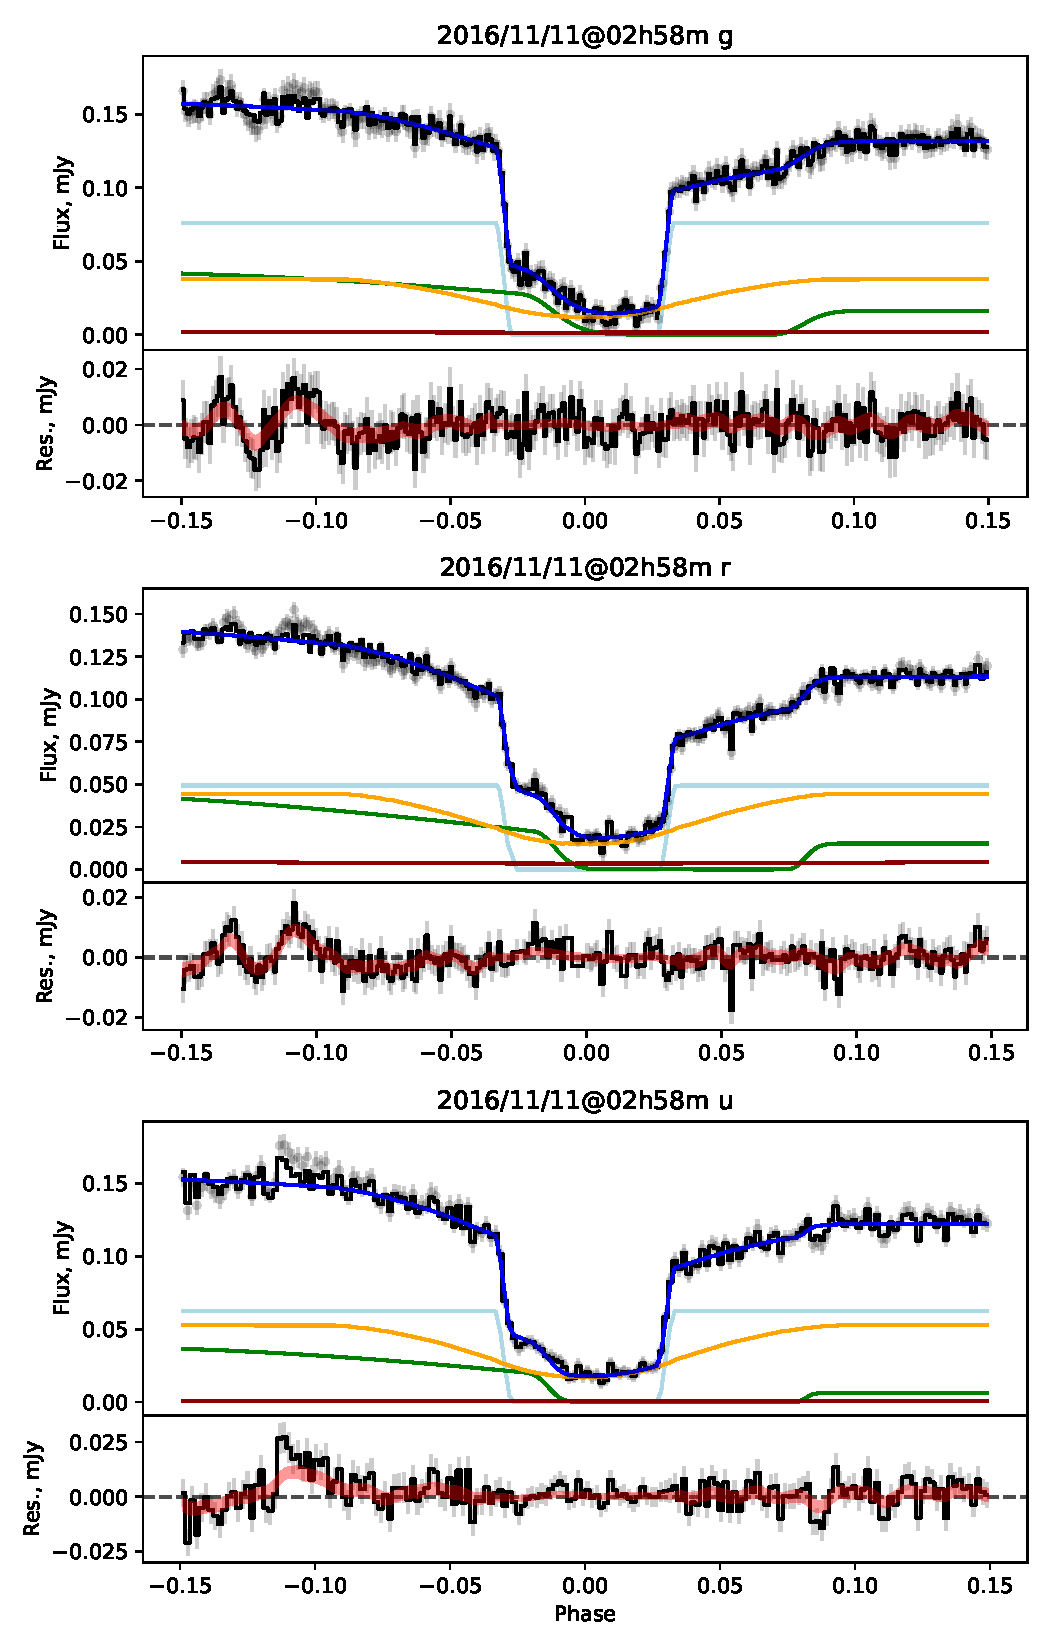
\includegraphics[width=\textwidth]{figures/results/AYFor/AYFor_3.pdf}
    \caption{AY For lightcurve models (cont.)}
    \label{fig:AYFor all lightcurves cont 2}
\end{figure}



\begin{figure}
    \centering
    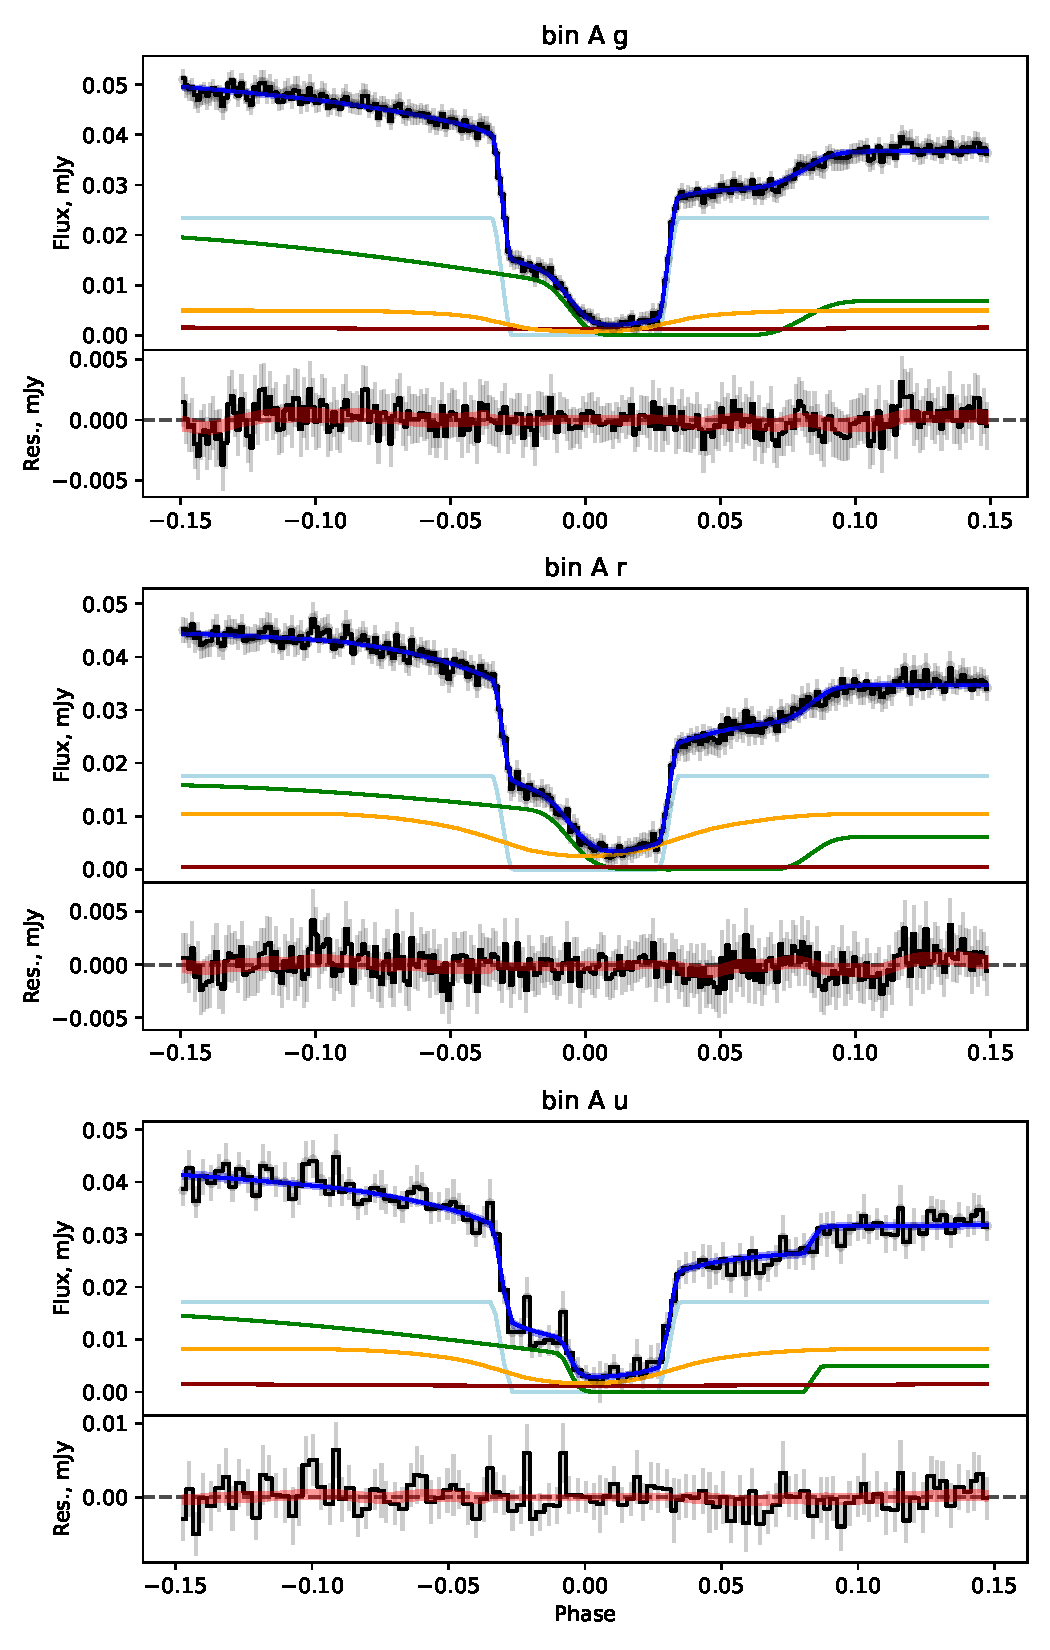
\includegraphics[width=\textwidth]{figures/results/CSS090102/CSS090102_1.pdf}
    \caption{CSS090102 lightcurve models. Symbols are the same as Figure~\ref{fig:ASASSN-17jf all lightcurves}}
    \label{fig:CSS090102 all lightcurves}
\end{figure}



\begin{figure}
    \centering
    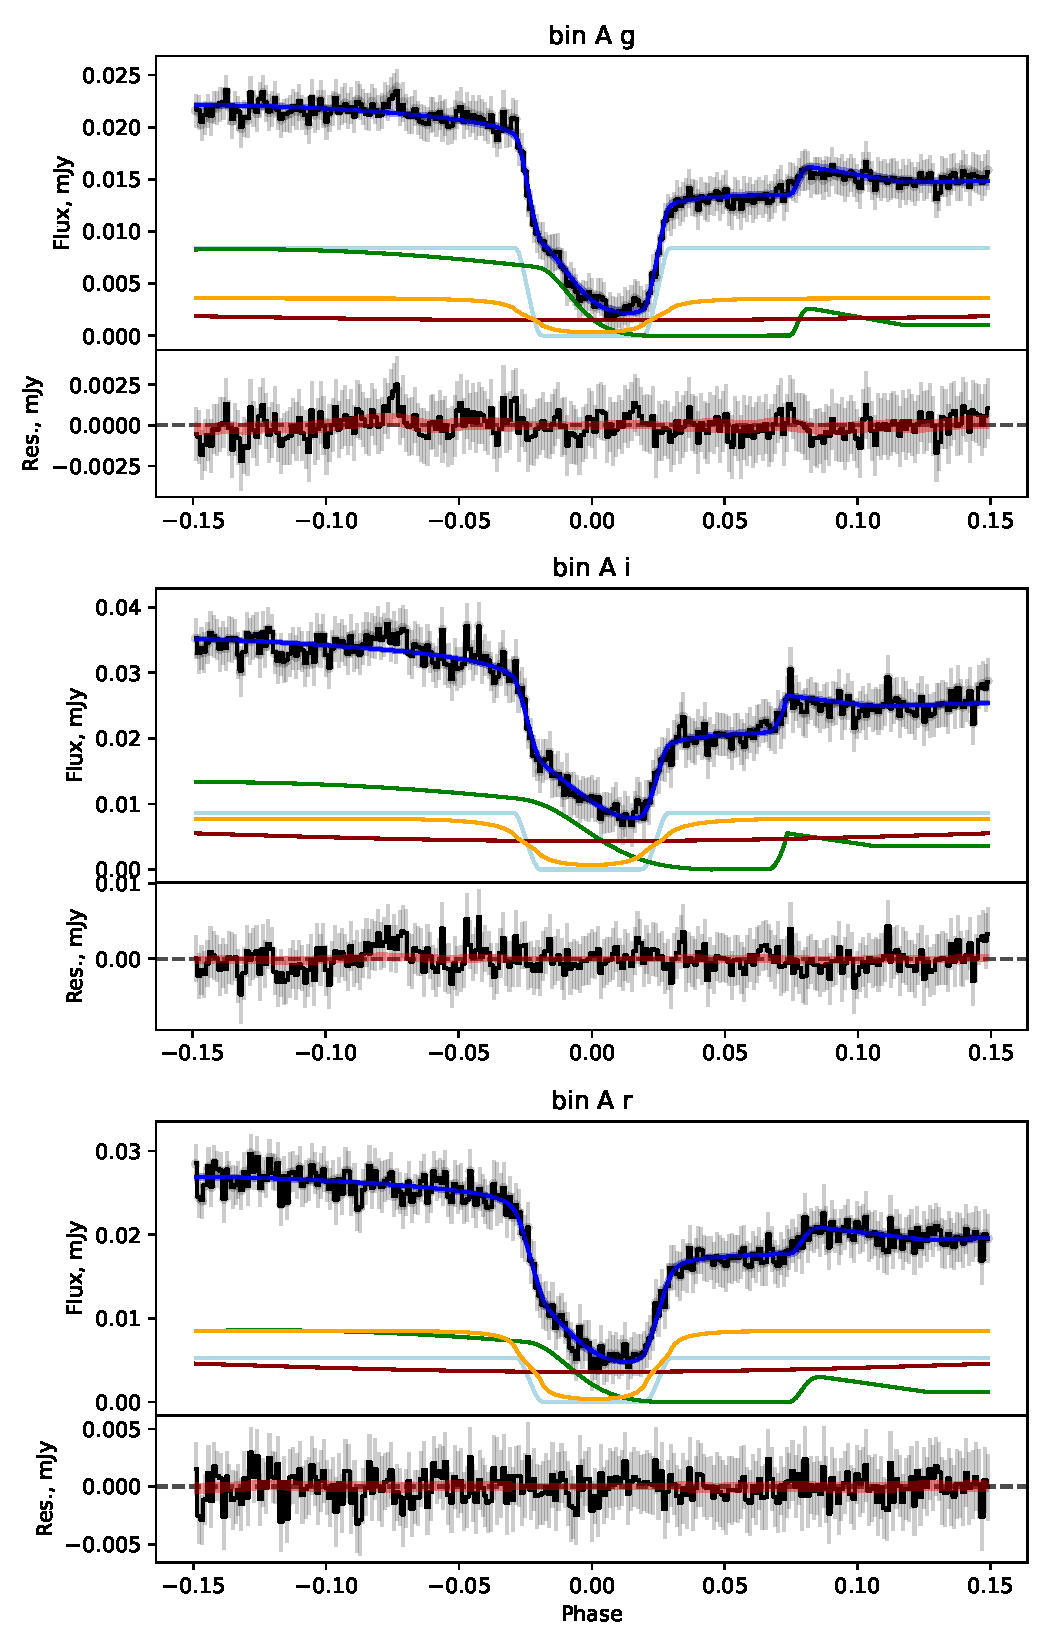
\includegraphics[width=\textwidth]{figures/results/CSS090419/CSS090419_1.pdf}
    \caption{CSS090419 lightcurve models. Symbols are the same as Figure~\ref{fig:ASASSN-17jf all lightcurves}}
    \label{fig:CSS090419 all lightcurves}
\end{figure}
\begin{figure}
    \centering
    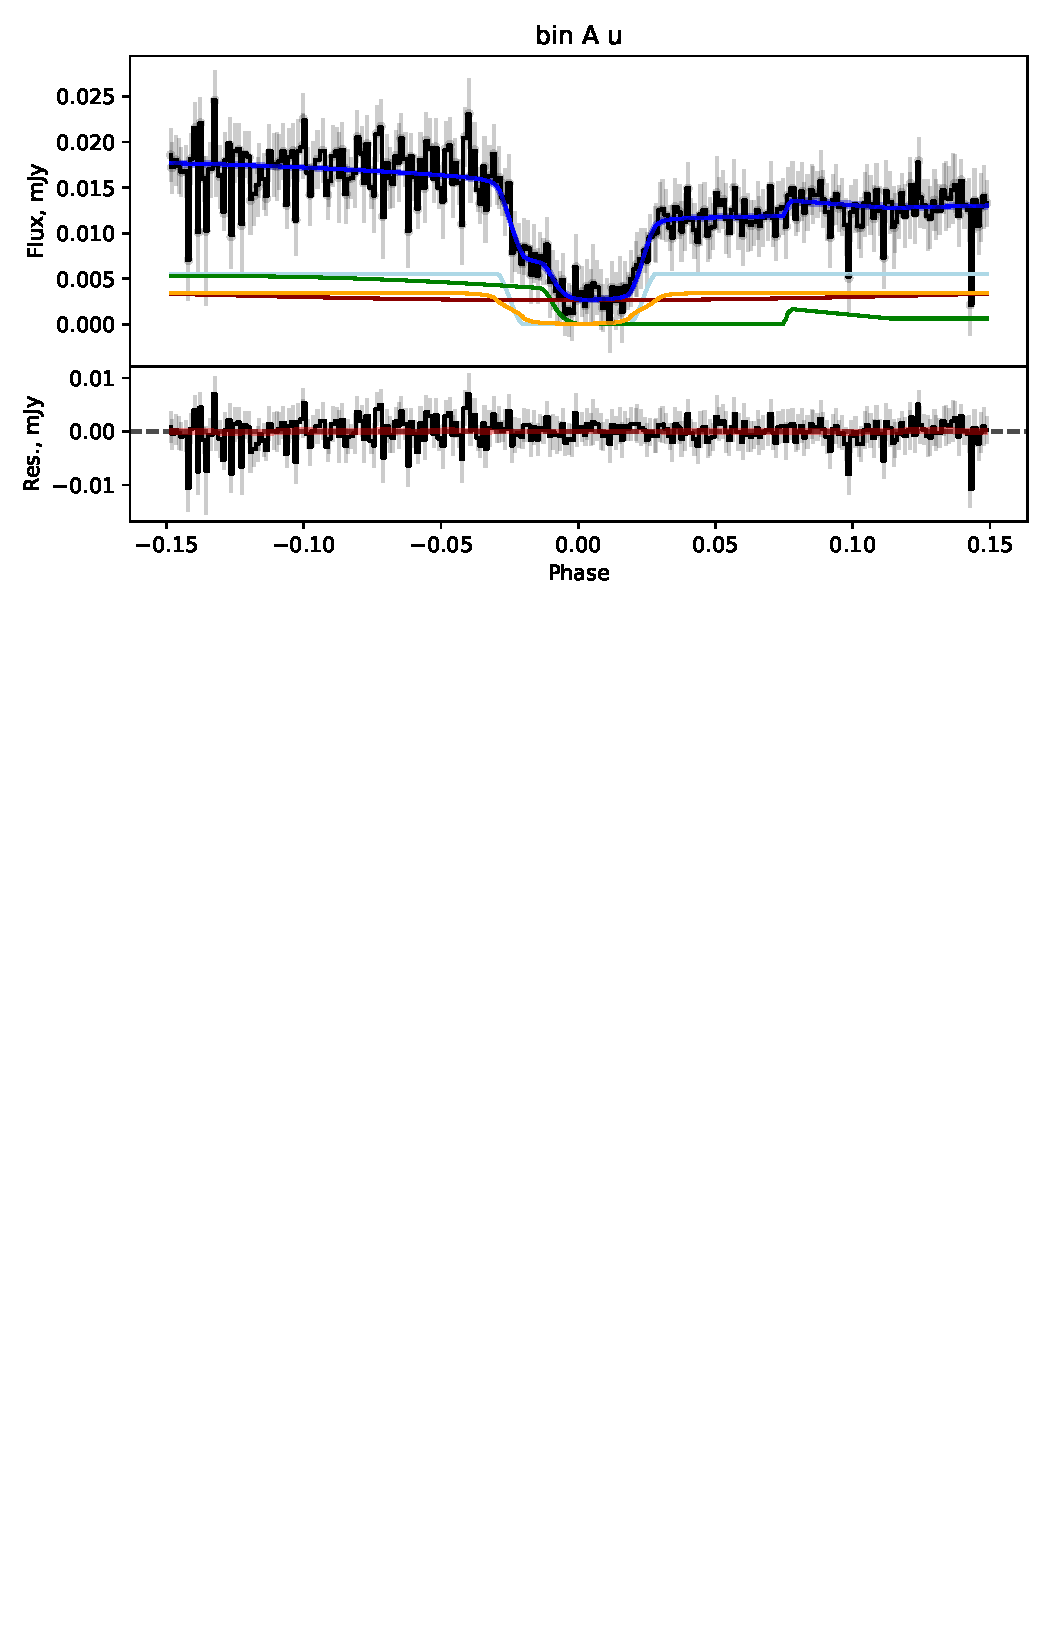
\includegraphics[width=\textwidth]{figures/results/CSS090419/CSS090419_2.pdf}
    \caption{CSS090419 lightcurve models (cont.)}
    \label{fig:CSS090419 all lightcurves cont 1}
\end{figure}



\begin{figure}
    \centering
    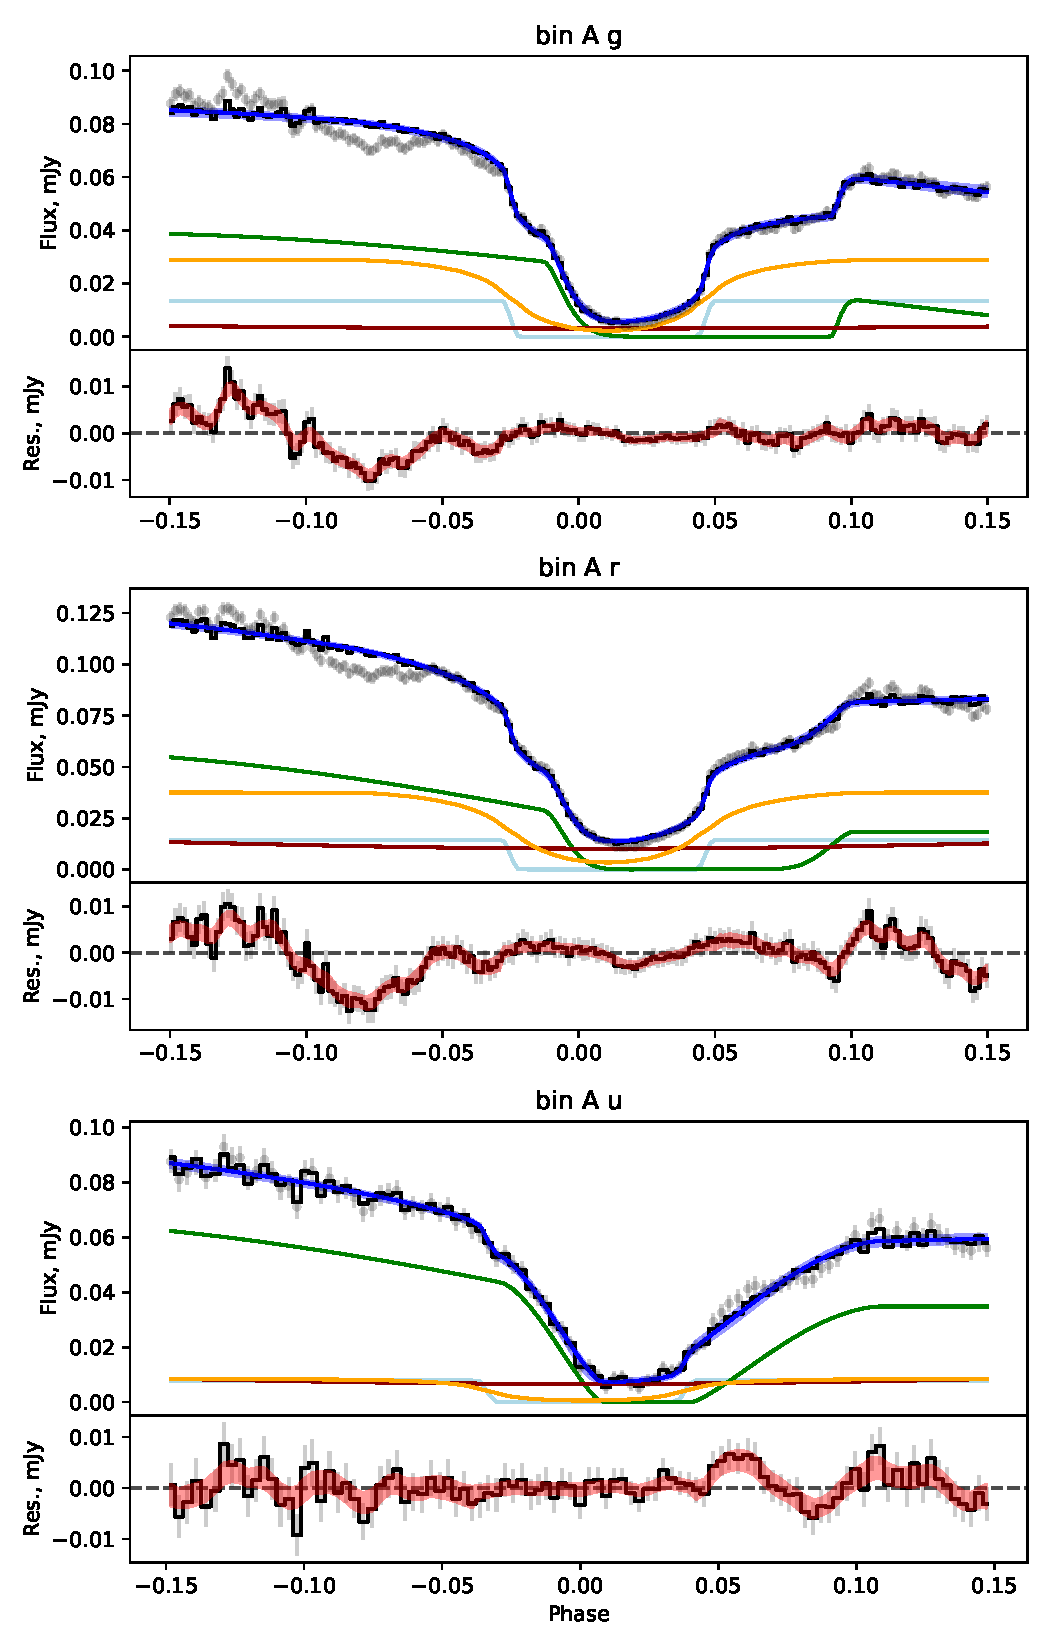
\includegraphics[width=\textwidth]{figures/results/CSS090622/CSS090622_1.pdf}
    \caption{CSS090622 lightcurve models. Symbols are the same as Figure~\ref{fig:ASASSN-17jf all lightcurves}}
    \label{fig:CSS090622 all lightcurves}
\end{figure}
\begin{figure}
    \centering
    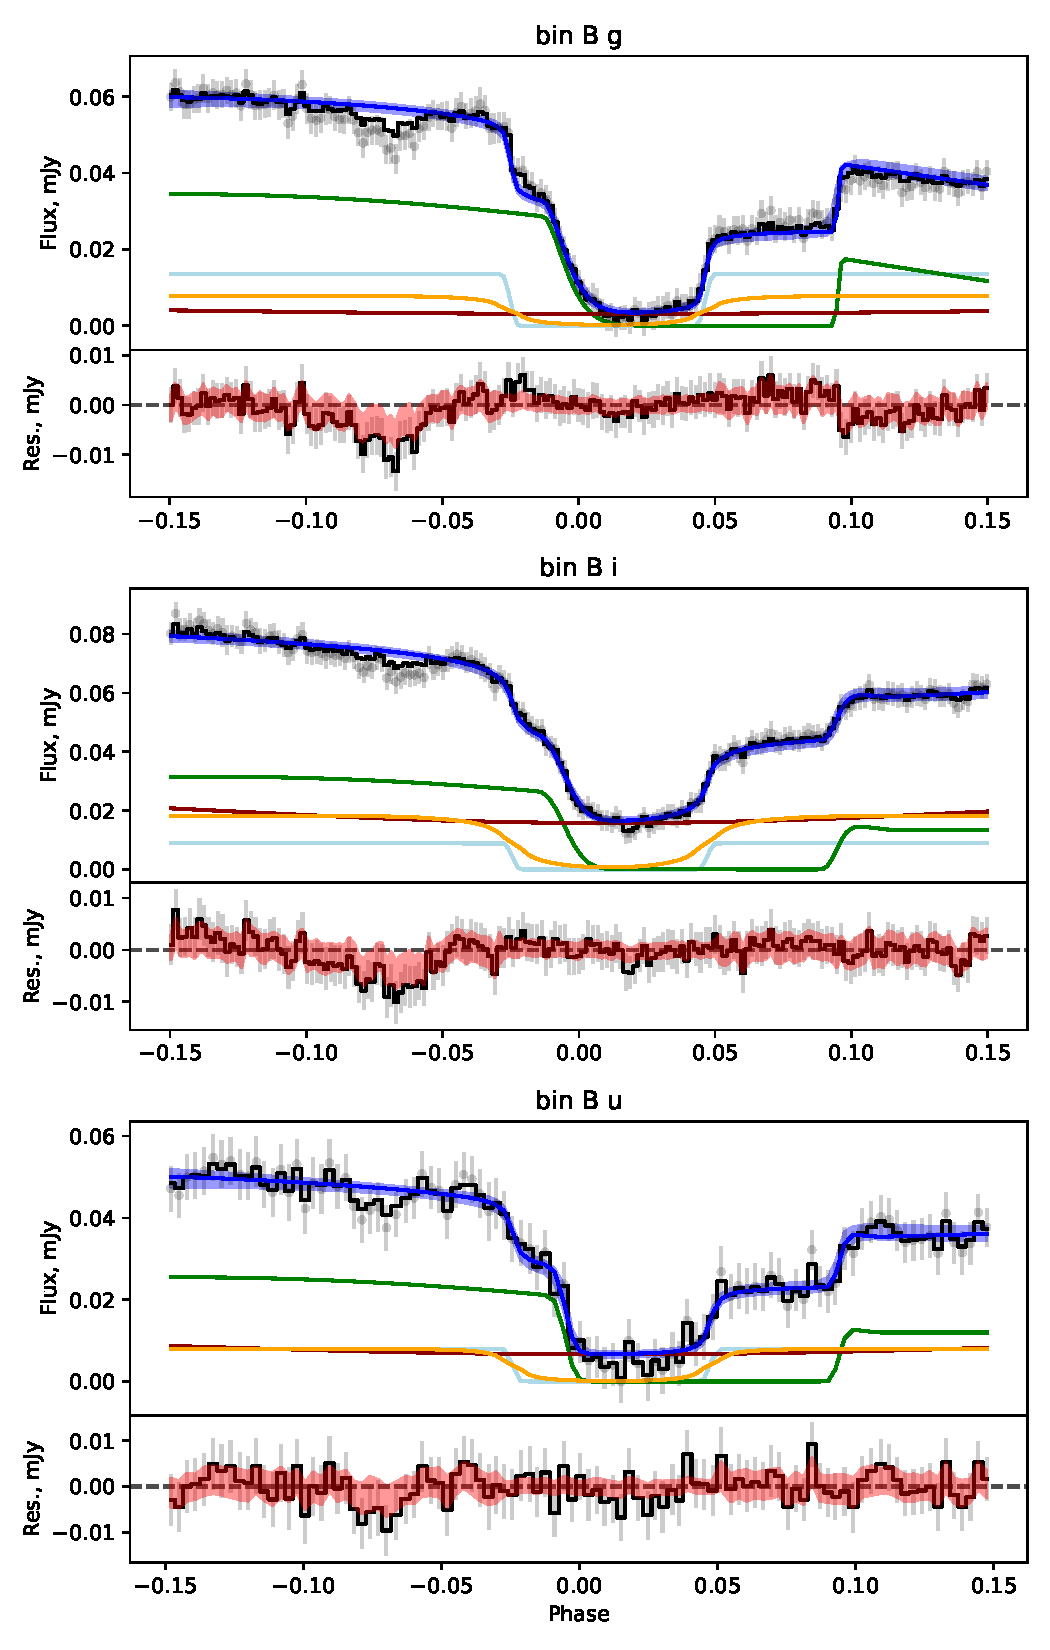
\includegraphics[width=\textwidth]{figures/results/CSS090622/CSS090622_2.pdf}
    \caption{CSS090622 lightcurve models (cont.)}
    \label{fig:CSS090622 all lightcurves cont 1}
\end{figure}



\begin{figure}
    \centering
    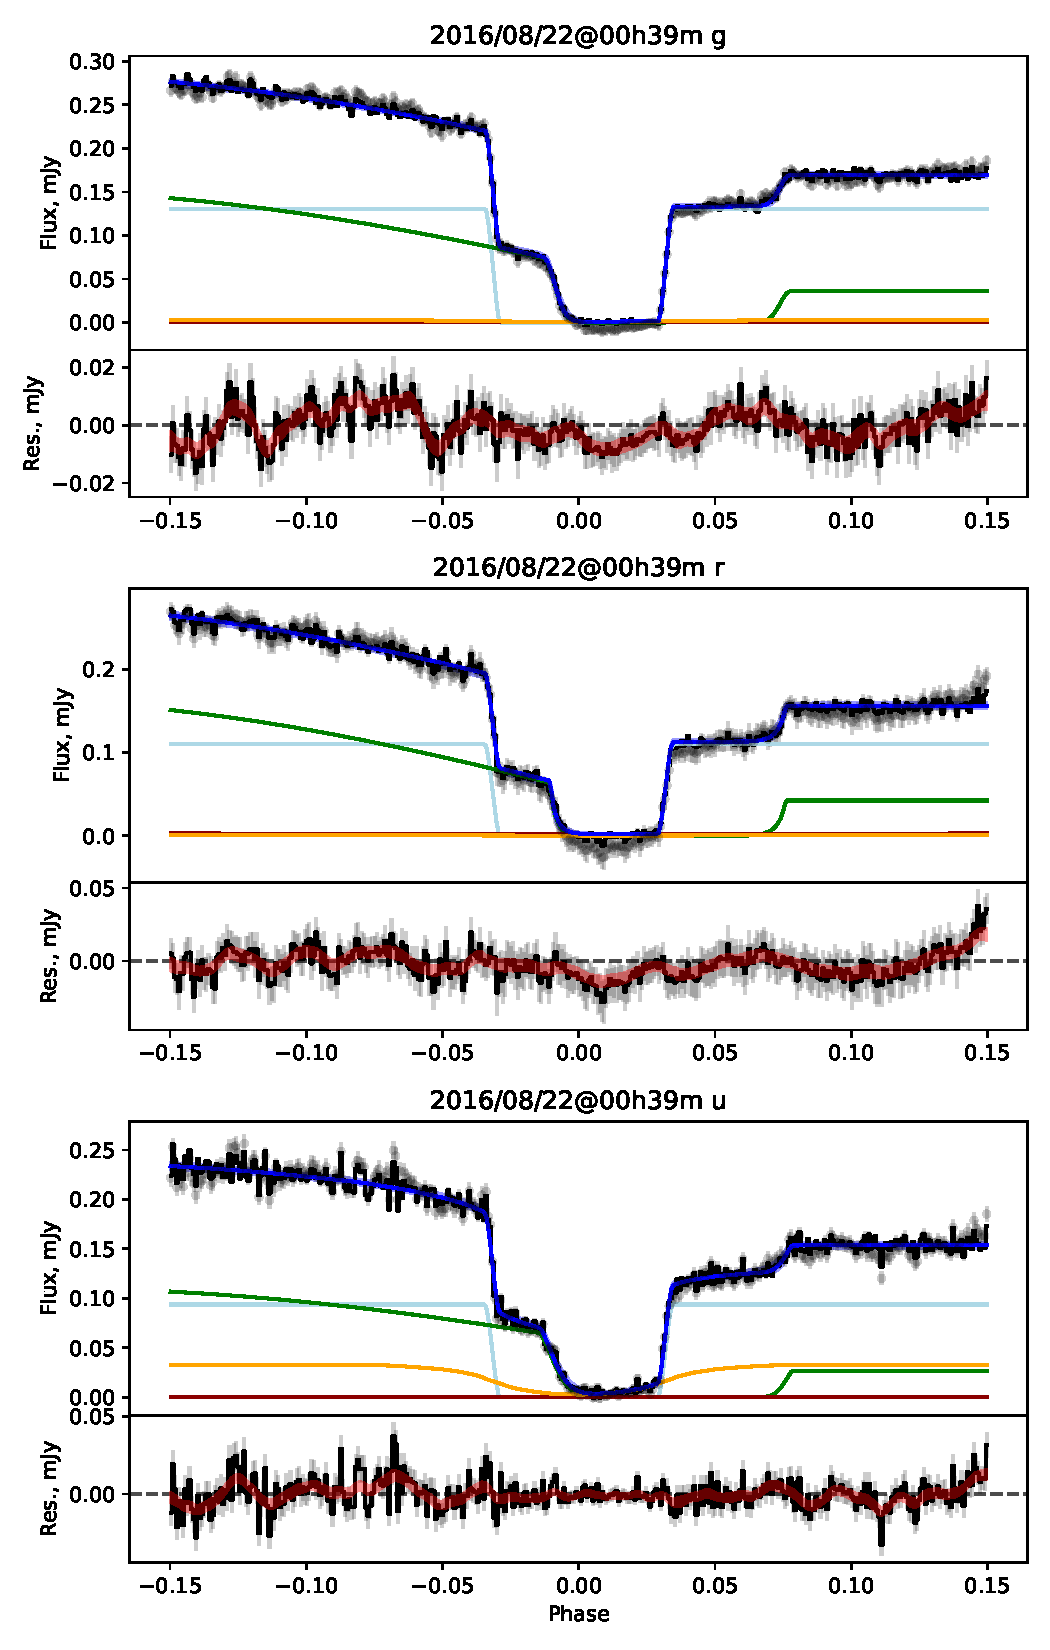
\includegraphics[width=\textwidth]{figures/results/OGLE82/OGLE82_1.pdf}
    \caption{OGLE82 lightcurve models. Symbols are the same as Figure~\ref{fig:ASASSN-17jf all lightcurves}}
    \label{fig:OGLE82 all lightcurves}
\end{figure}
\begin{figure}
    \centering
    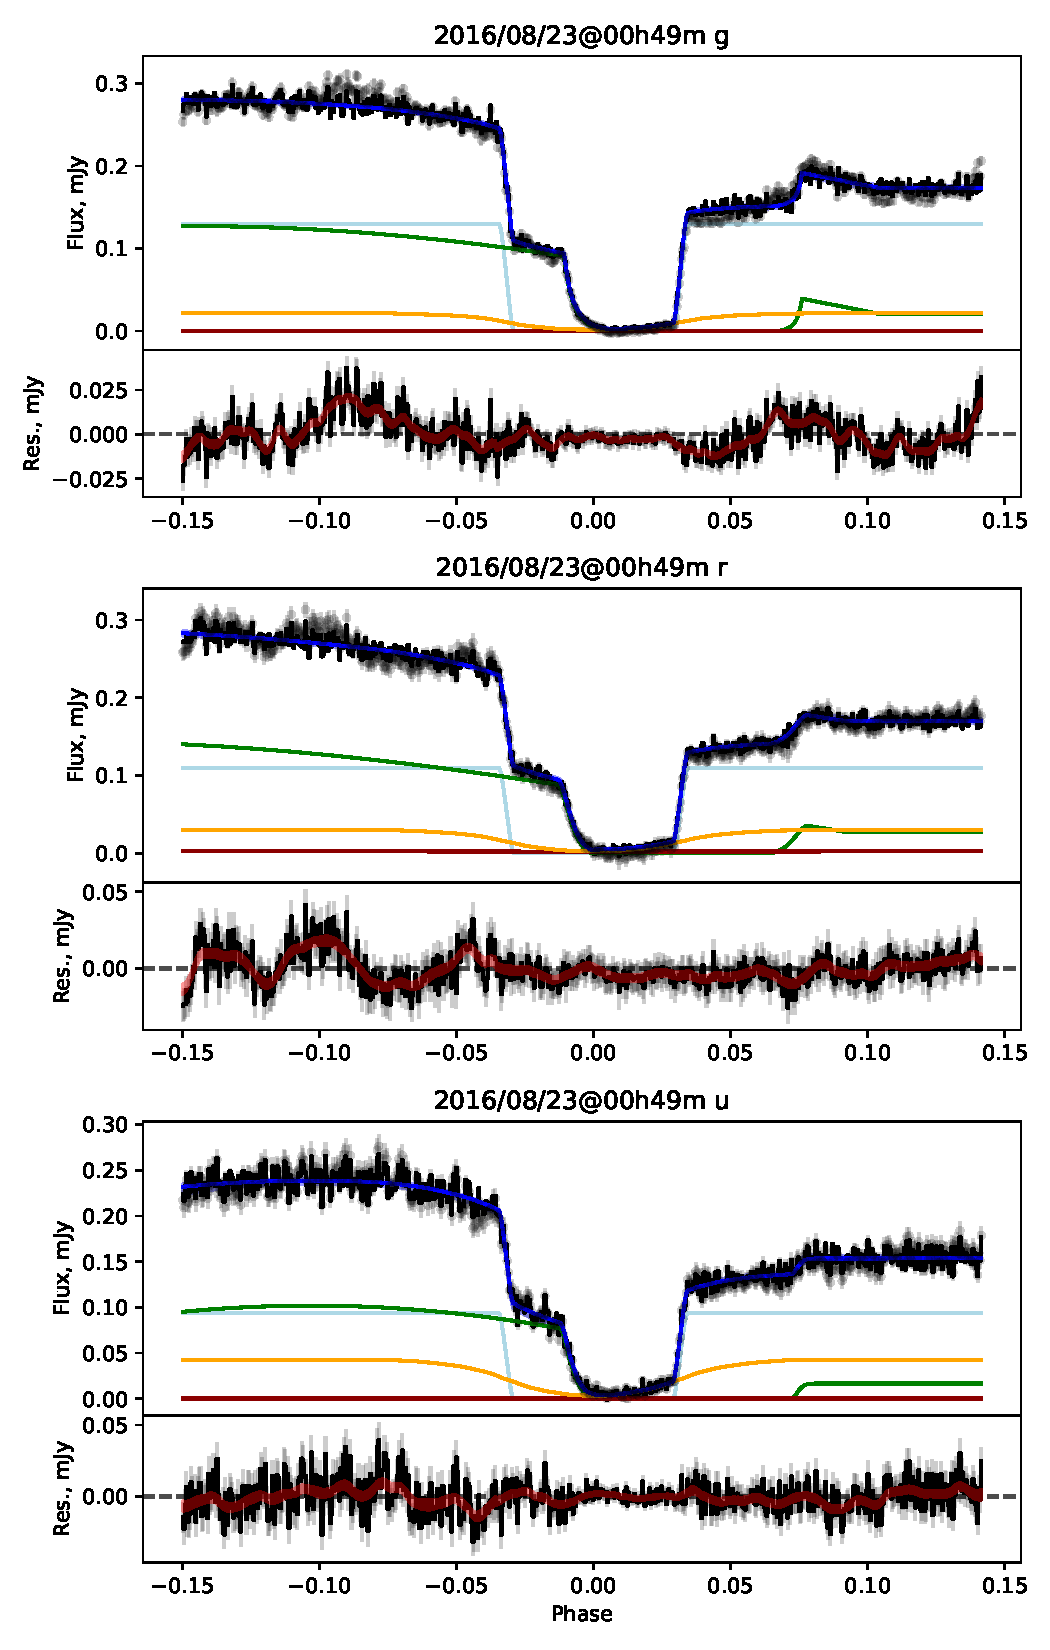
\includegraphics[width=\textwidth]{figures/results/OGLE82/OGLE82_2.pdf}
    \caption{OGLE82 lightcurve models (cont.)}
    \label{fig:OGLE82 all lightcurves cont 1}
\end{figure}



\begin{figure}
    \centering
    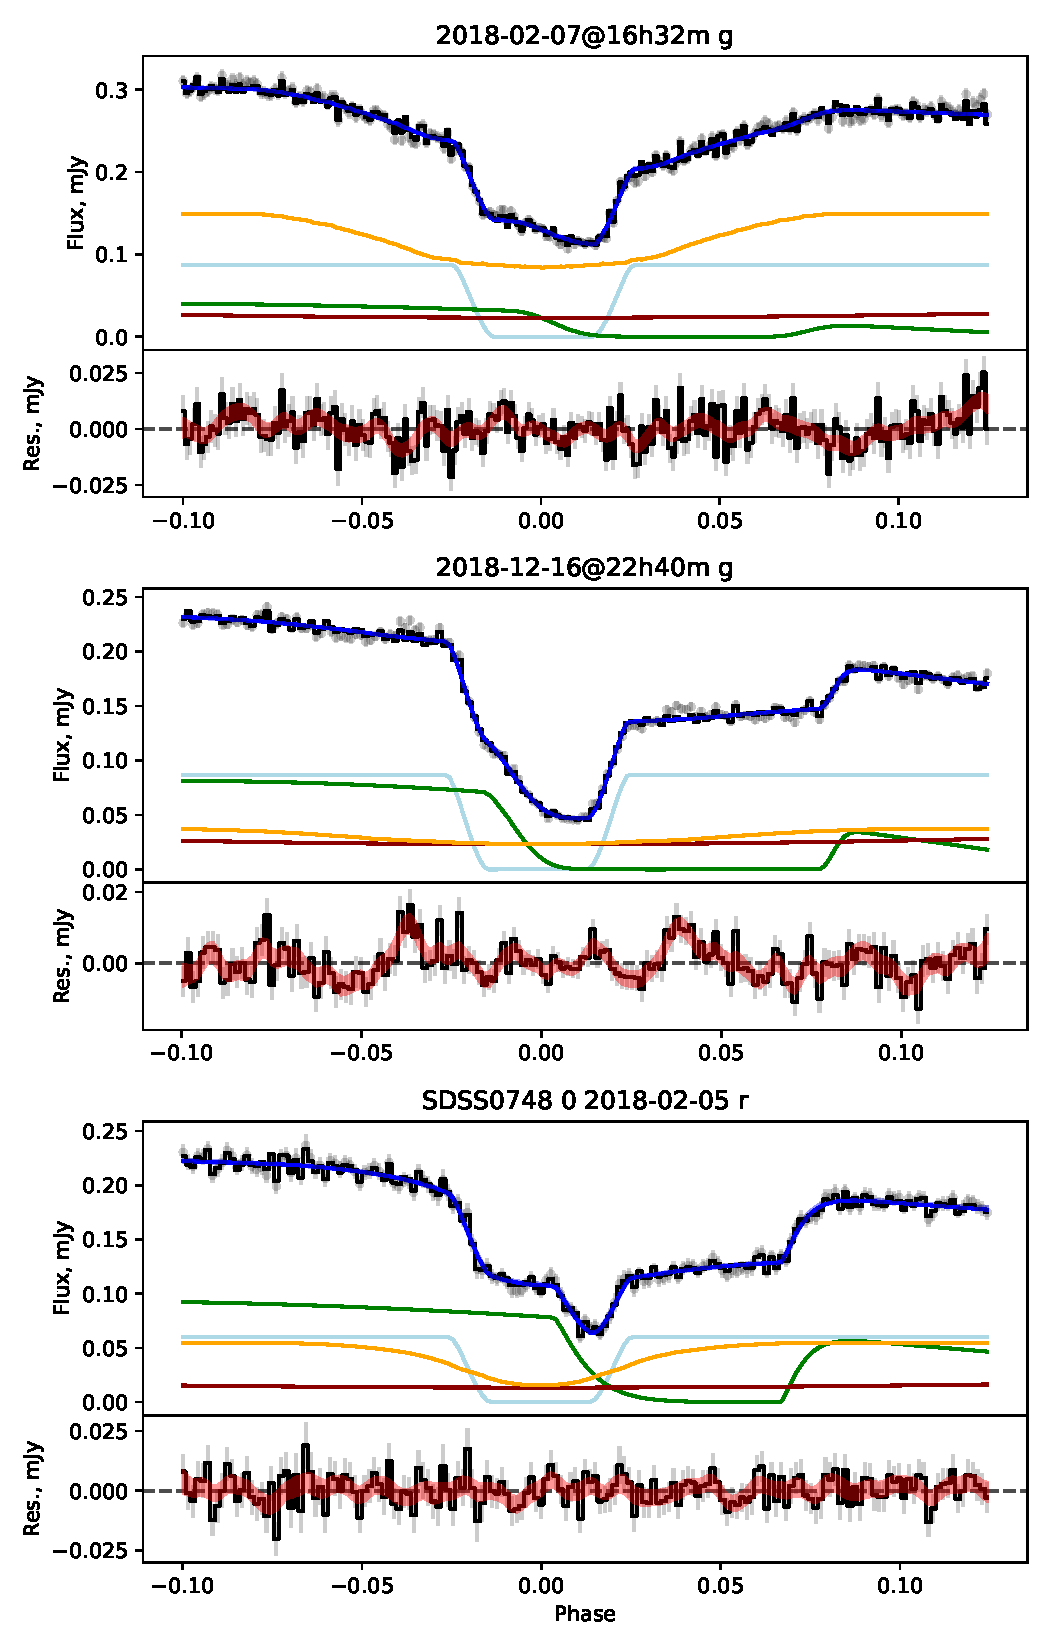
\includegraphics[width=\textwidth]{figures/results/SDSS0748/SDSS0748_1.pdf}
    \caption{SDSS J0748 lightcurve models. Symbols are the same as Figure~\ref{fig:ASASSN-17jf all lightcurves}}
    \label{fig:SDSS J0748 all lightcurves}
\end{figure}
\begin{figure}
    \centering
    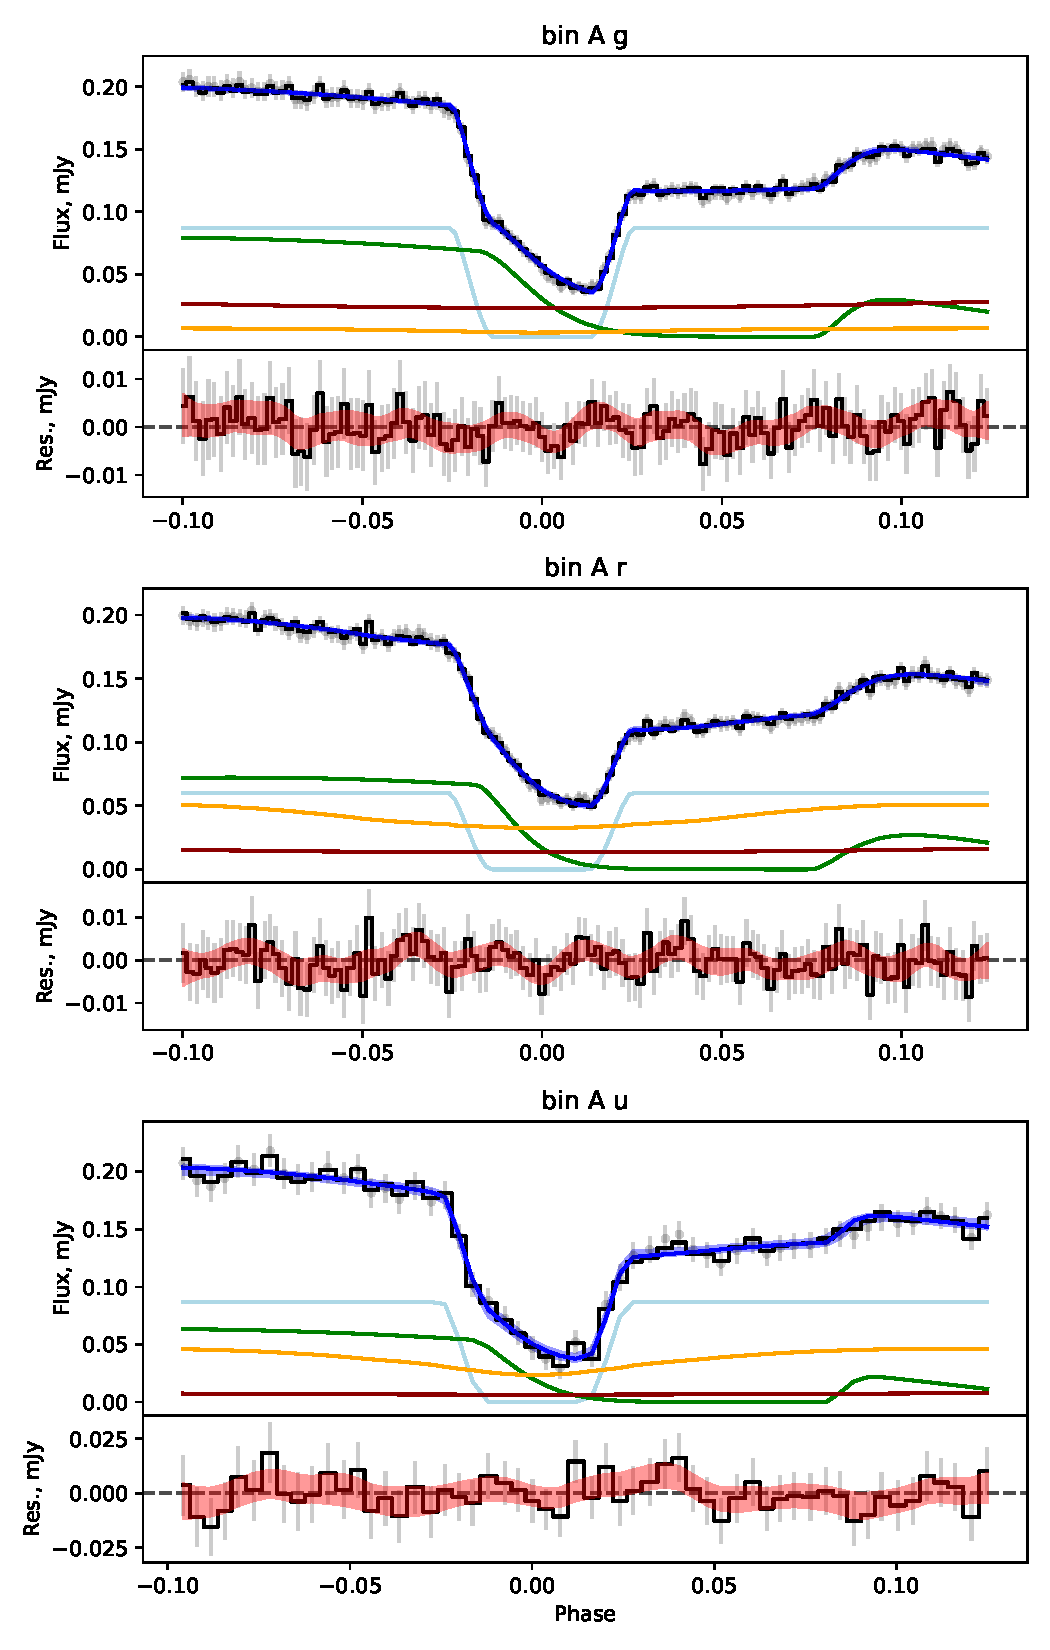
\includegraphics[width=\textwidth]{figures/results/SDSS0748/SDSS0748_2.pdf}
    \caption{SDSS J0748 lightcurve models (cont.)}
    \label{fig:SDSS J0748 all lightcurves cont 1}
\end{figure}
\begin{figure}
    \centering
    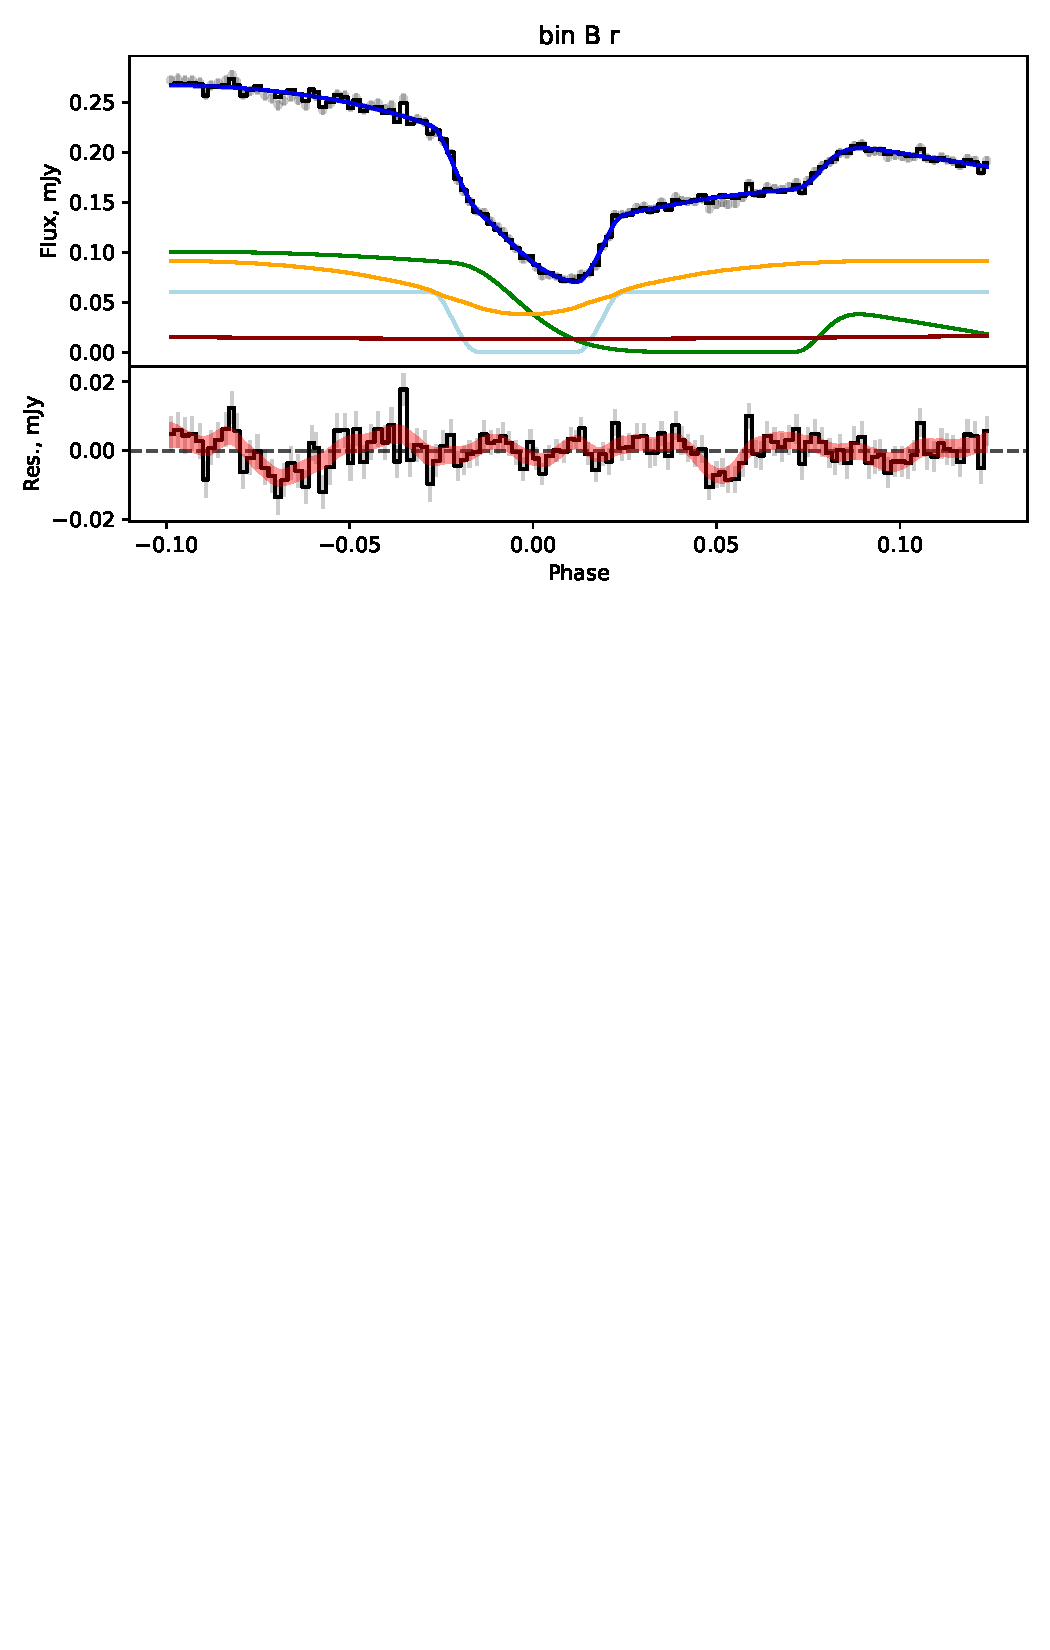
\includegraphics[width=\textwidth]{figures/results/SDSS0748/SDSS0748_3.pdf}
    \caption{SDSS J0748 lightcurve models (cont.)}
    \label{fig:SDSS J0748 all lightcurves cont 2}
\end{figure}



\begin{figure}
    \centering
    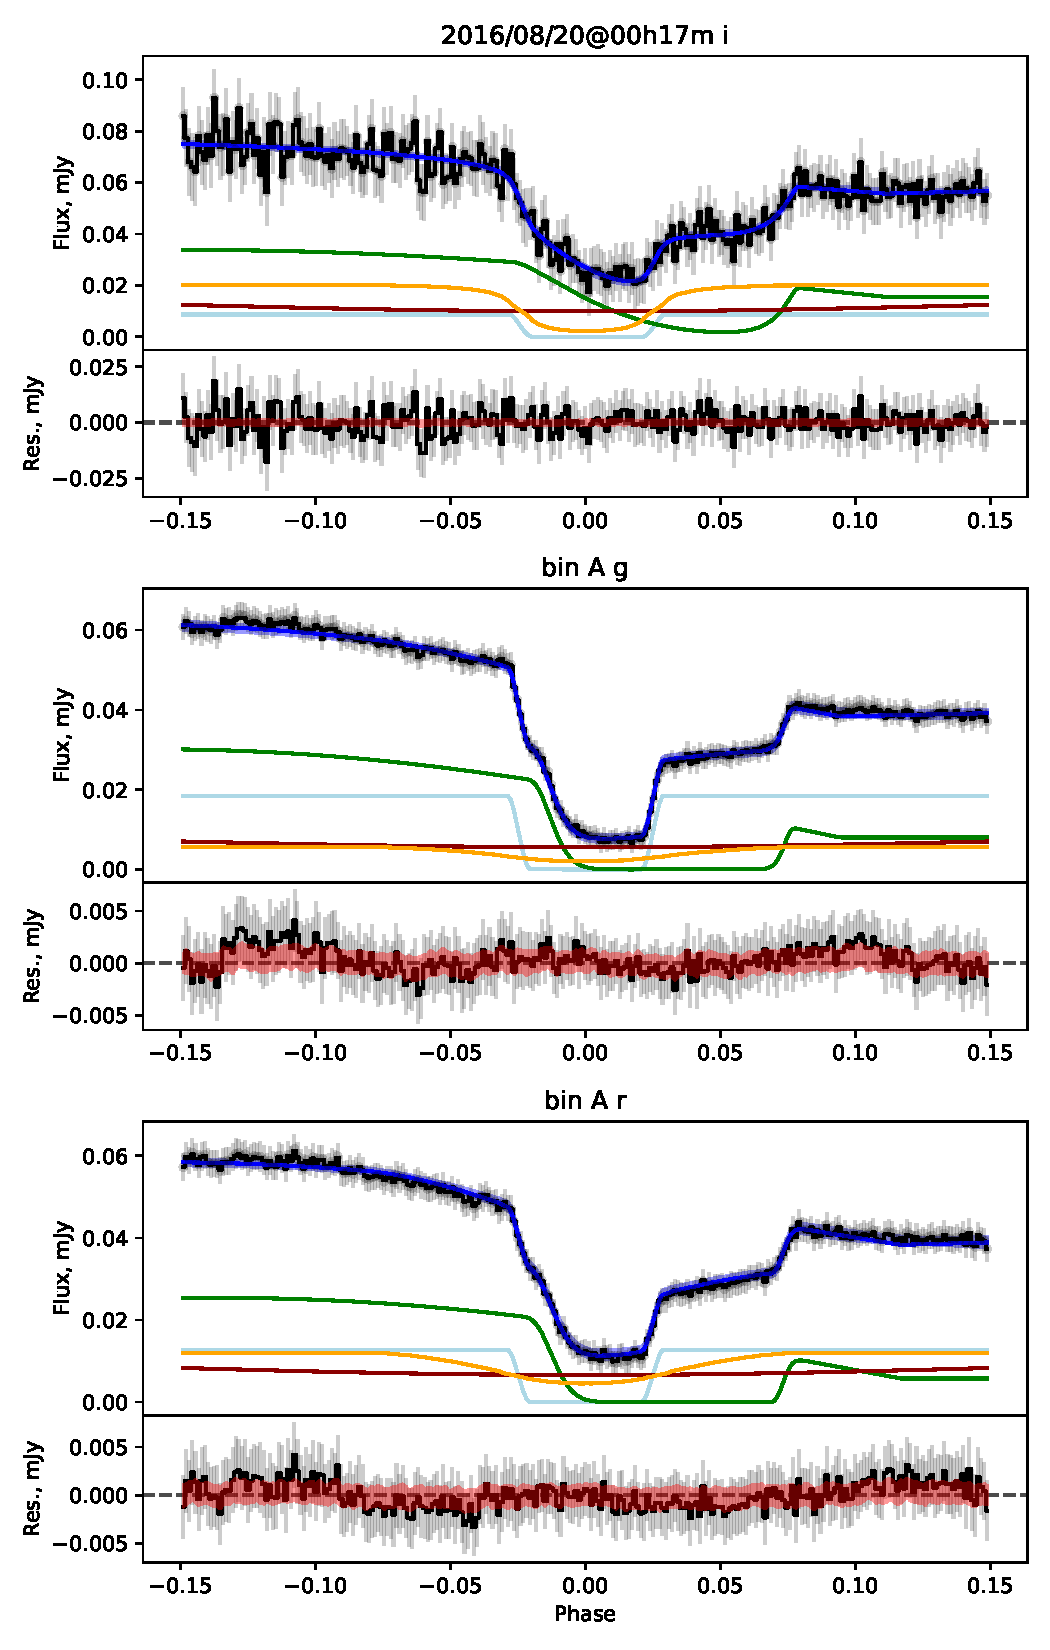
\includegraphics[width=\textwidth]{figures/results/ASASSN-15pb/ASASSN-15pb_1.pdf}
    \caption{ASASSN-15pb lightcurve models. Symbols are the same as Figure~\ref{fig:ASASSN-17jf all lightcurves}}
    \label{fig:ASASSN-15pb all lightcurves}
\end{figure}
\begin{figure}
    \centering
    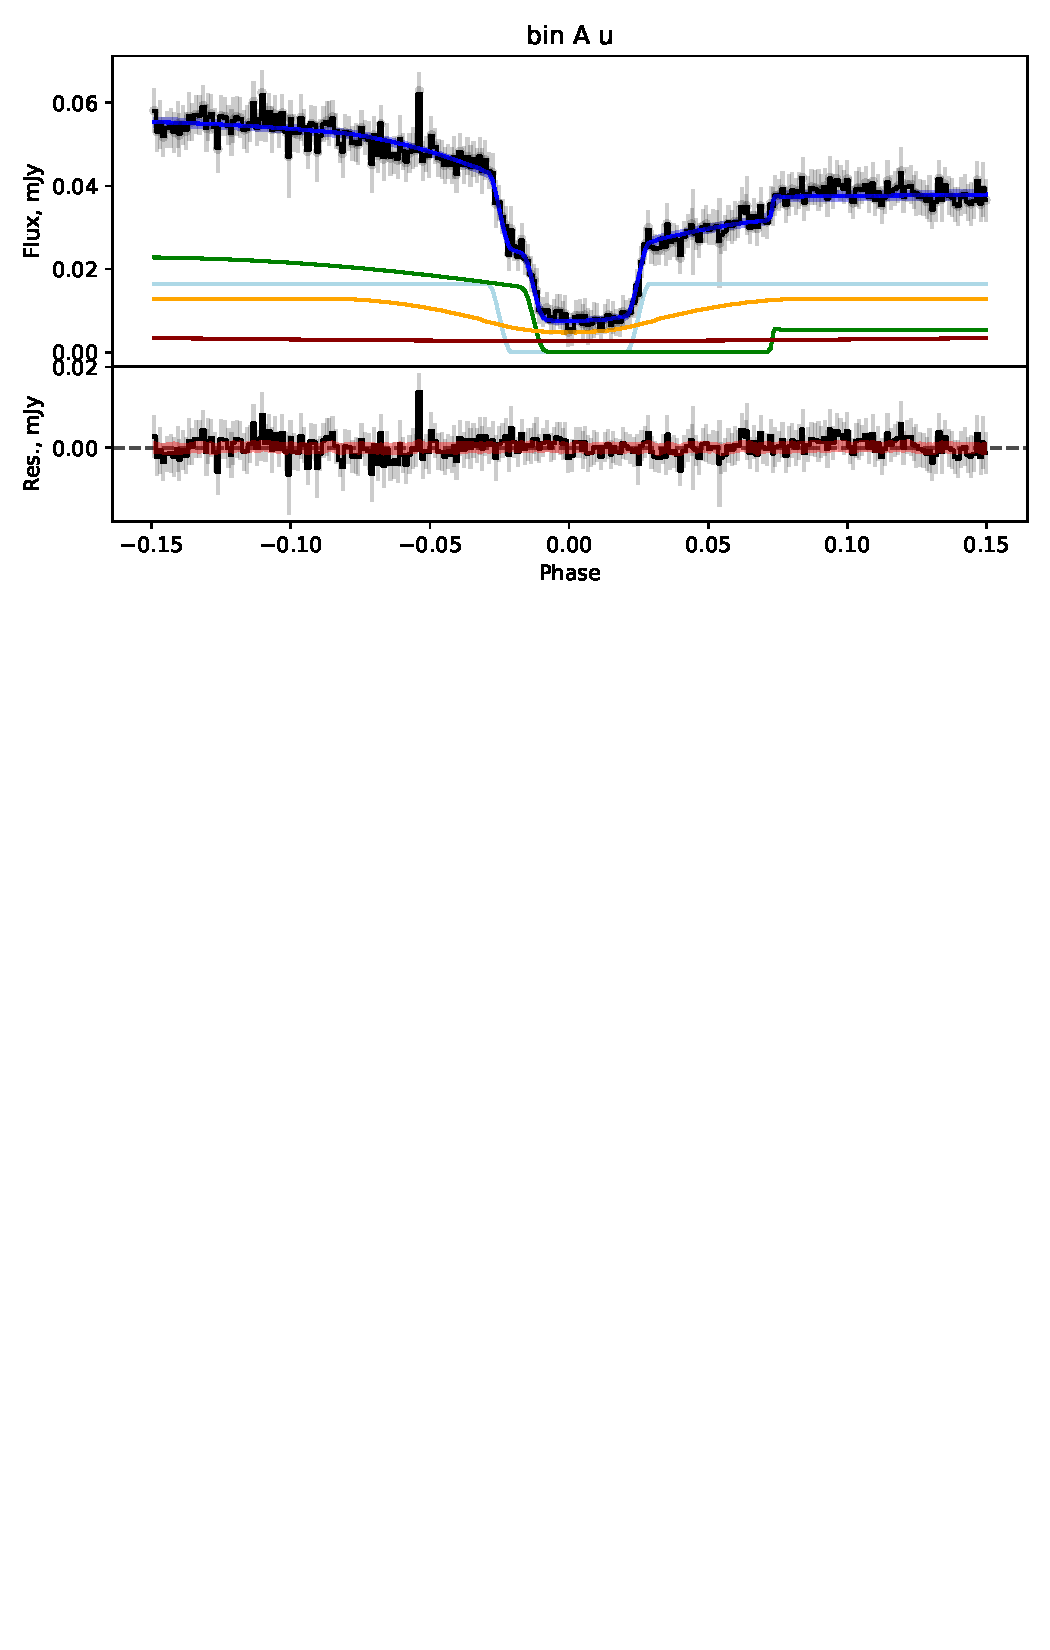
\includegraphics[width=\textwidth]{figures/results/ASASSN-15pb/ASASSN-15pb_2.pdf}
    \caption{ASASSN-15pb lightcurve models (cont.)}
    \label{fig:ASASSN-15pb all lightcurves cont 1}
\end{figure}



\begin{figure}
    \centering
    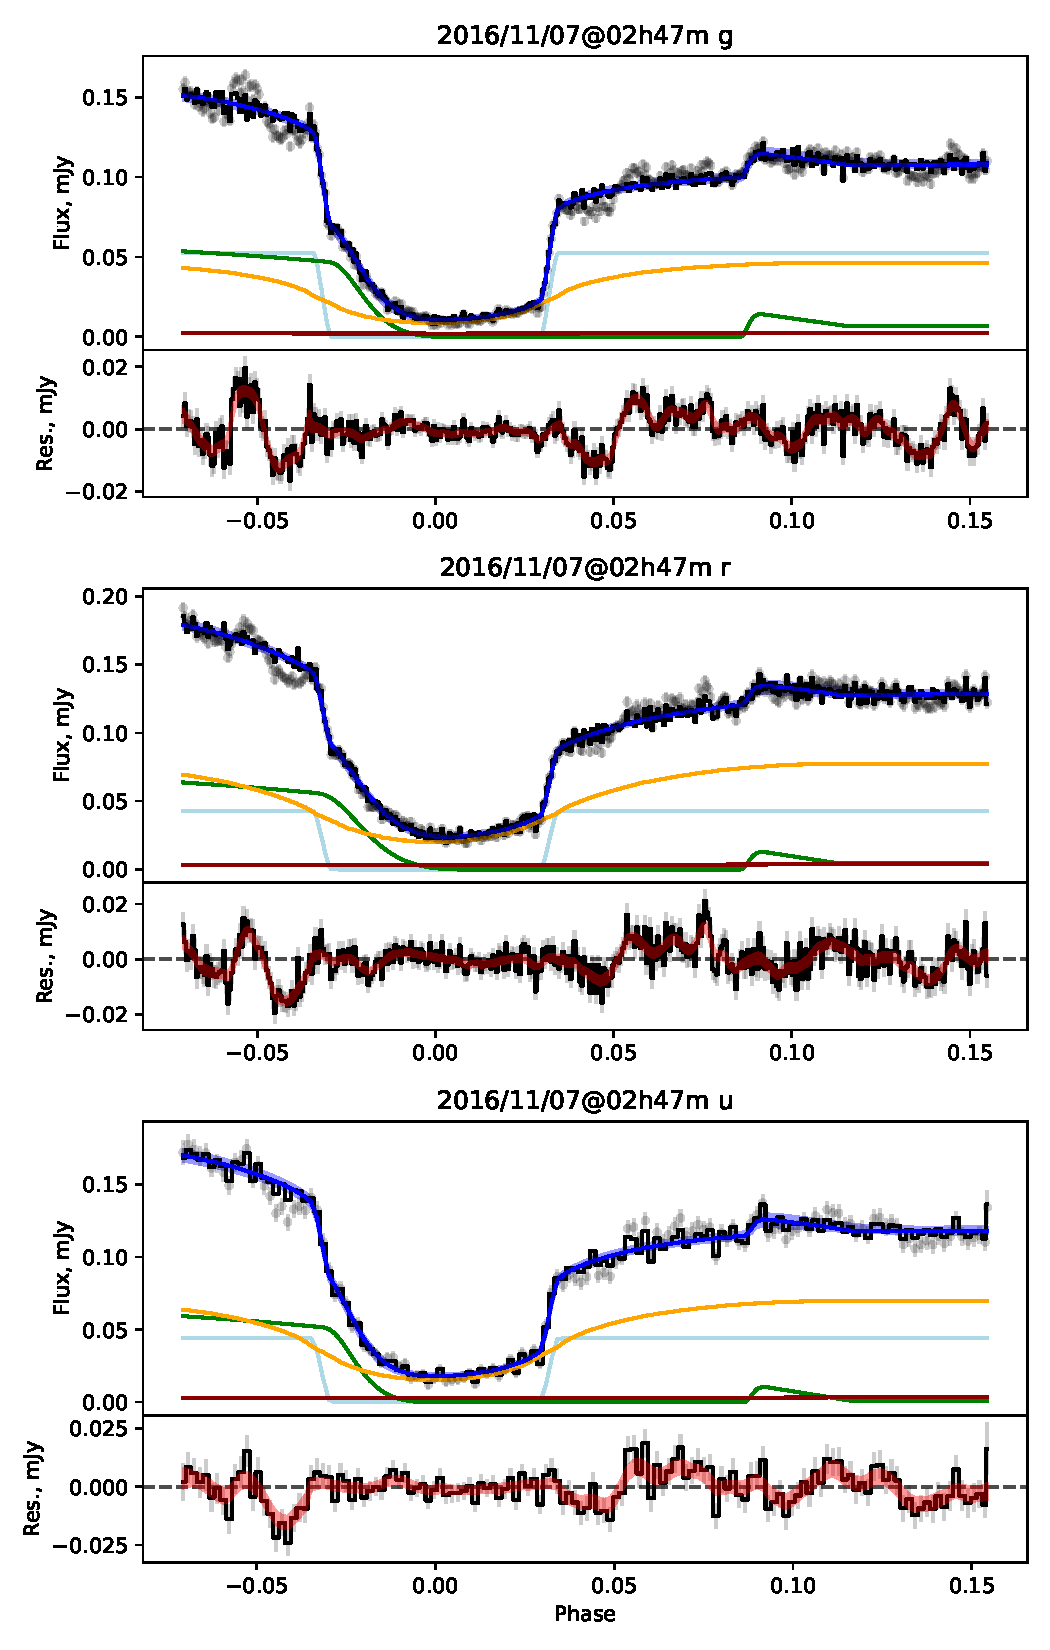
\includegraphics[width=\textwidth]{figures/results/MASOT0014/MASOT0014_1.pdf}
    \caption{MAS0014 lightcurve models. Symbols are the same as Figure~\ref{fig:ASASSN-17jf all lightcurves}}
    \label{fig:MAS0014 all lightcurves}
\end{figure}
\begin{figure}
    \centering
    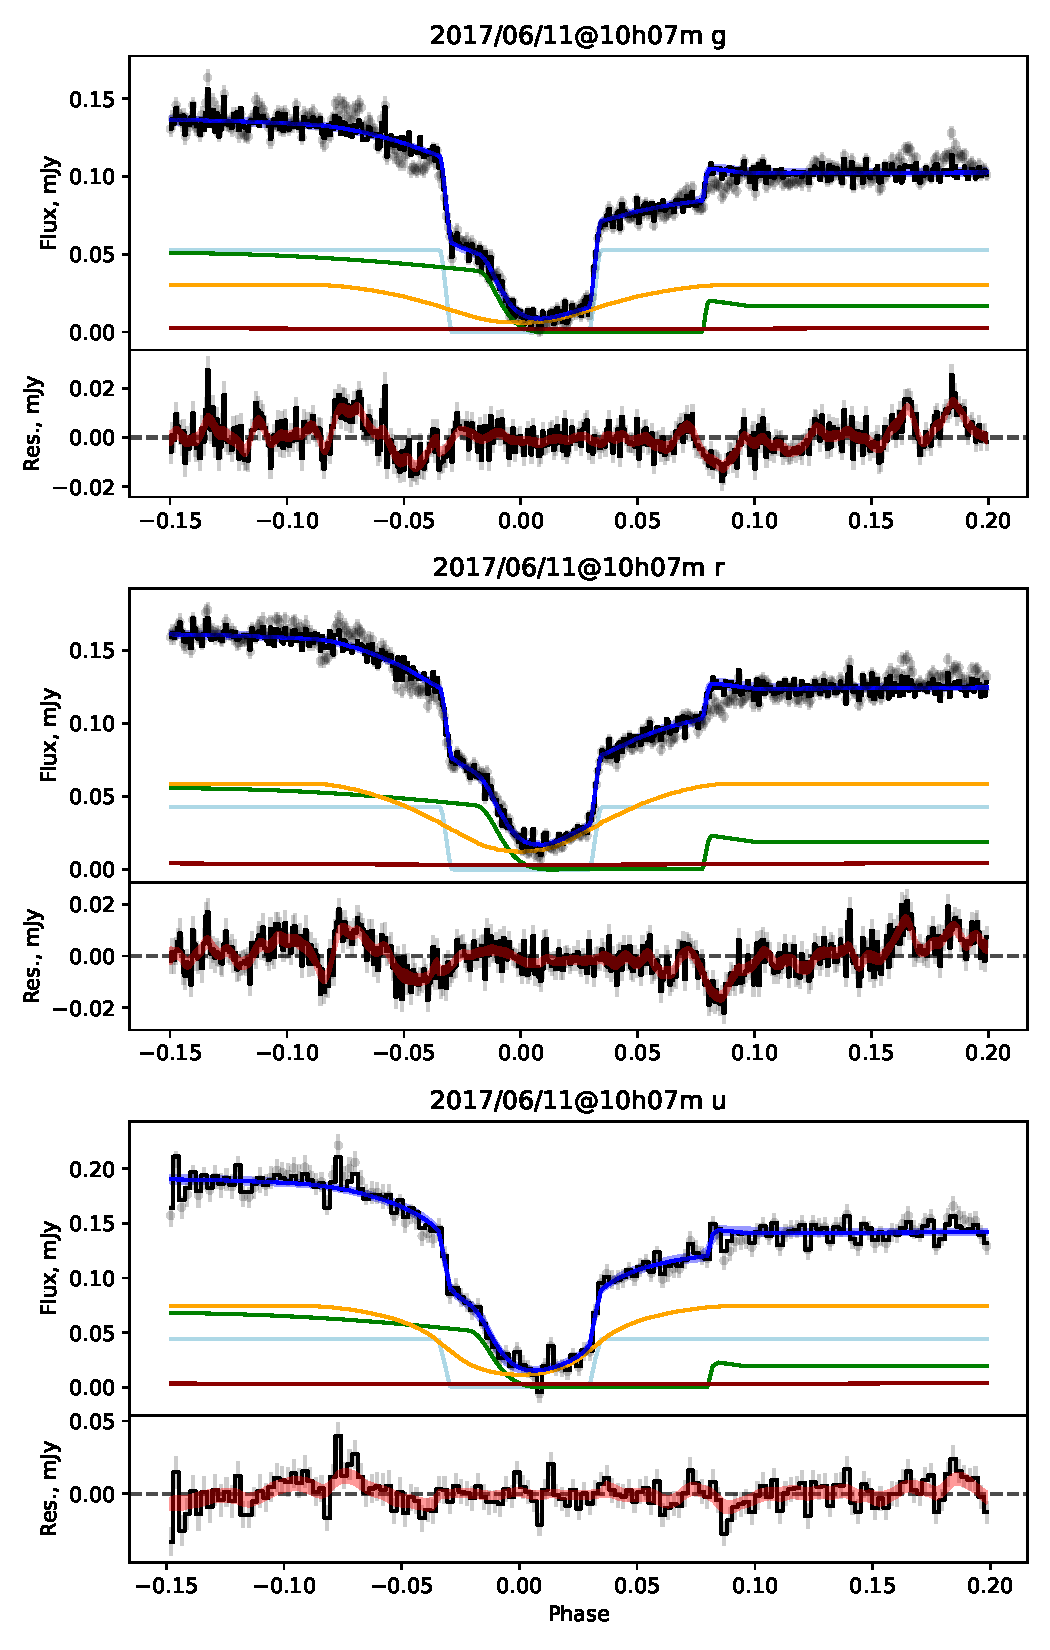
\includegraphics[width=\textwidth]{figures/results/MASOT0014/MASOT0014_2.pdf}
    \caption{MAS0014 lightcurve models (cont.)}
    \label{fig:MAS0014 all lightcurves cont 1}
\end{figure}
\begin{figure}
    \centering
    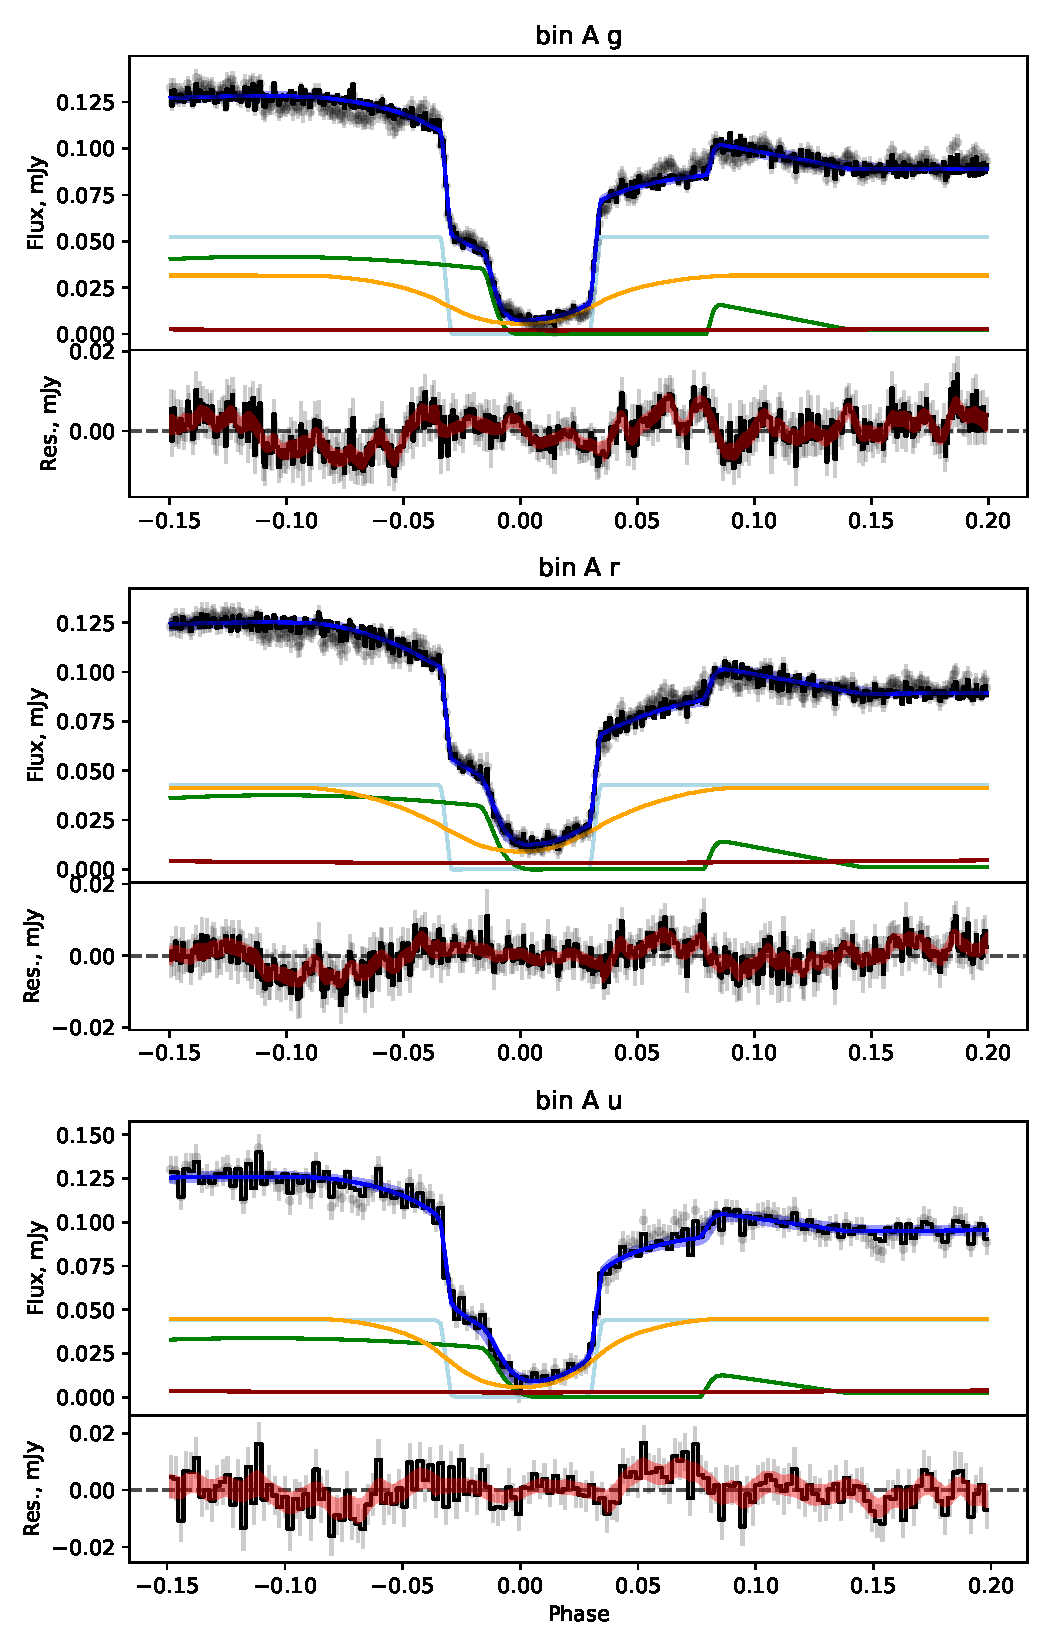
\includegraphics[width=\textwidth]{figures/results/MASOT0014/MASOT0014_3.pdf}
    \caption{MAS0014 lightcurve models (cont.)}
    \label{fig:MAS0014 all lightcurves cont 2}
\end{figure}


\begin{figure}
    \centering
    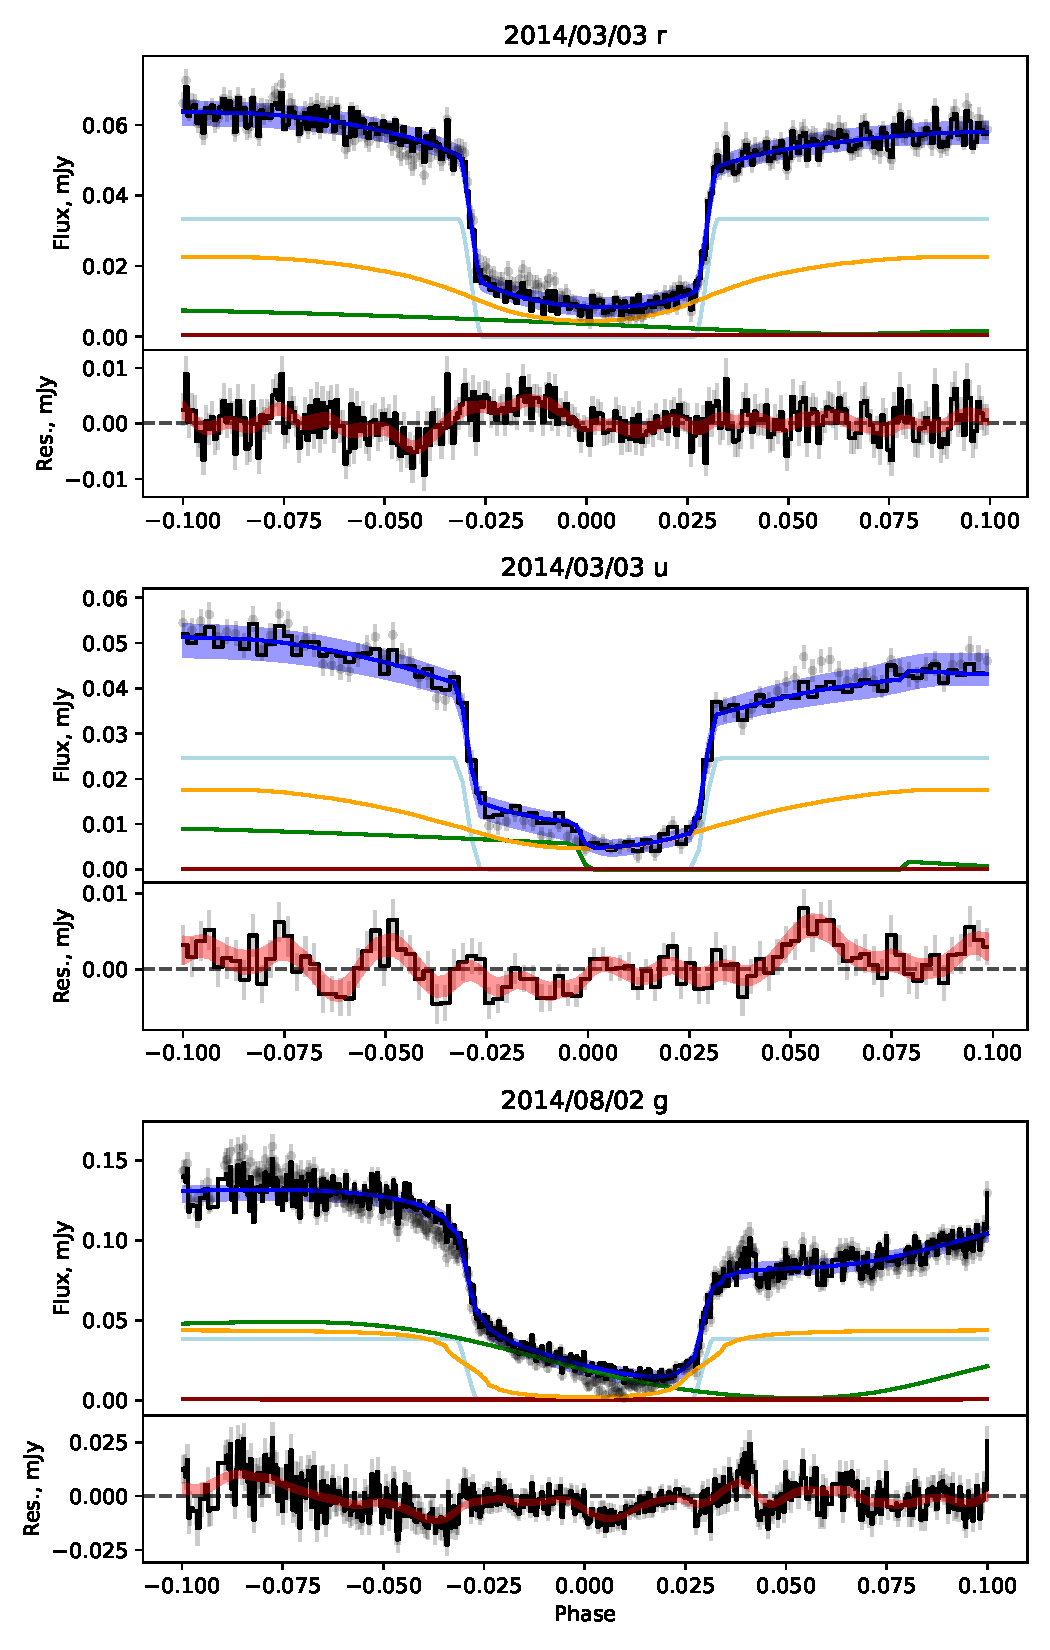
\includegraphics[width=\textwidth]{figures/results/SDSS1524/SDSS1524_1.pdf}
    \caption{SDSS J1524 lightcurve models. Symbols are the same as Figure~\ref{fig:ASASSN-17jf all lightcurves}}
    \label{fig:SDSS1524 all lightcurves}
\end{figure}
\begin{figure}
    \centering
    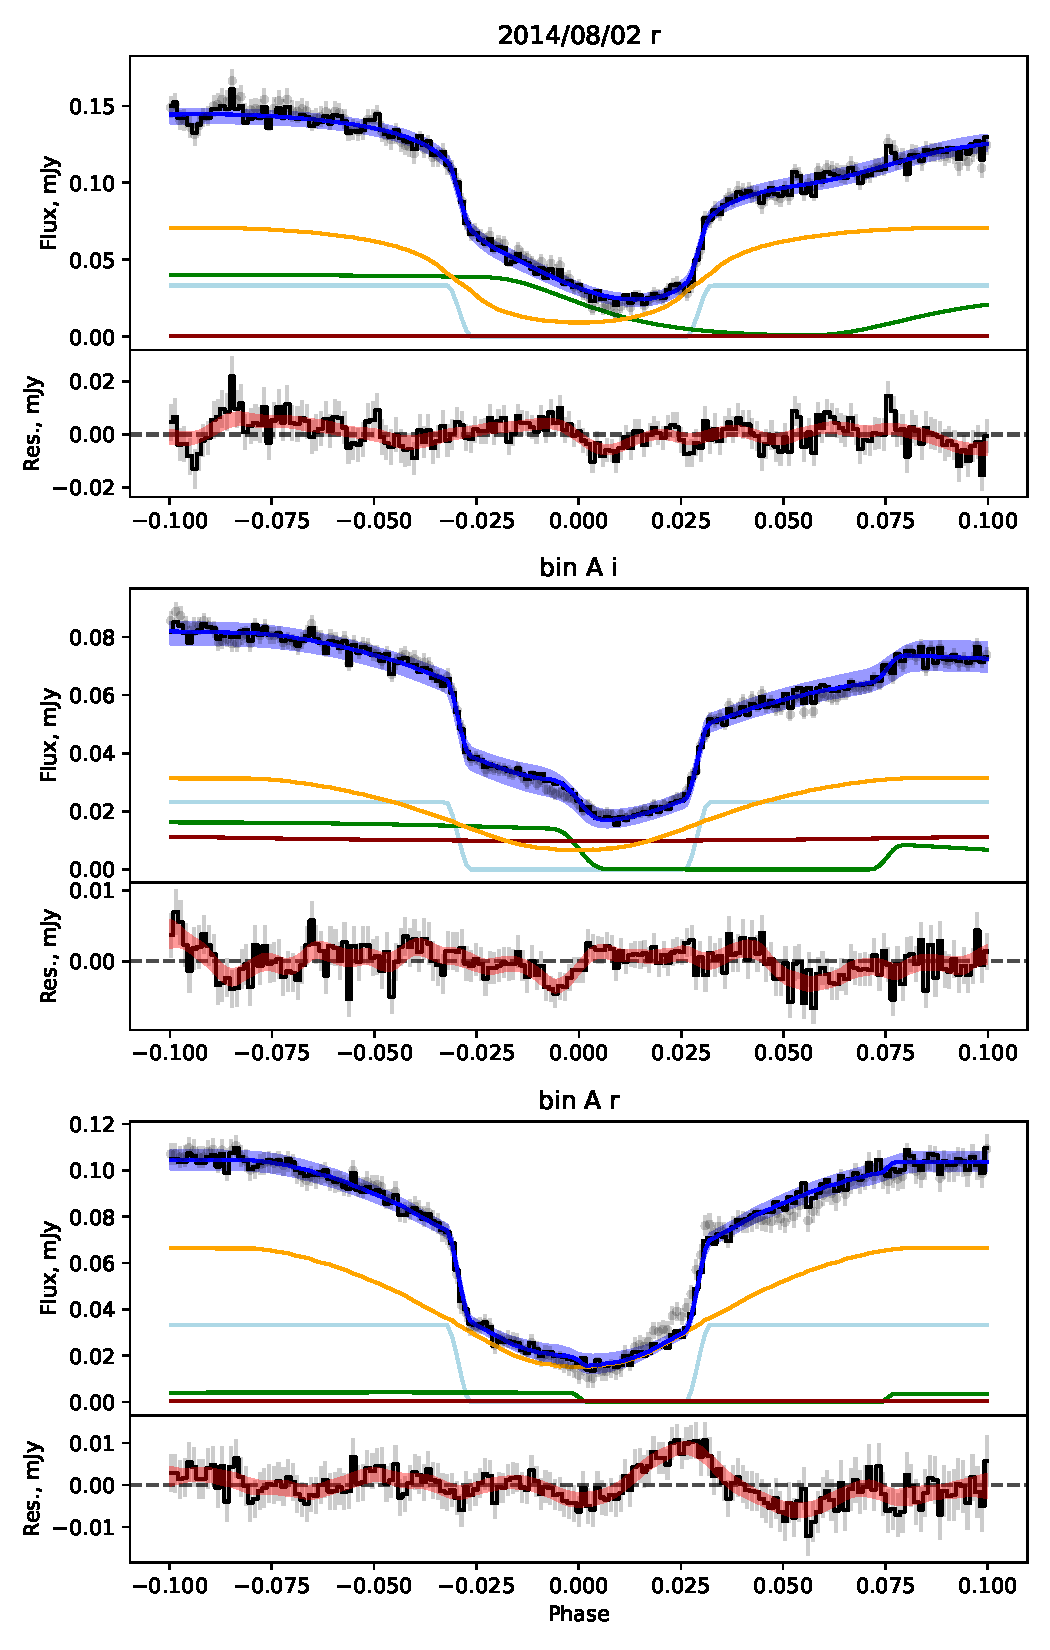
\includegraphics[width=\textwidth]{figures/results/SDSS1524/SDSS1524_2.pdf}
    \caption{SDSS J1524 lightcurve models (cont.)}
    \label{fig:SDSS1524 all lightcurves cont 1}
\end{figure}
\begin{figure}
    \centering
    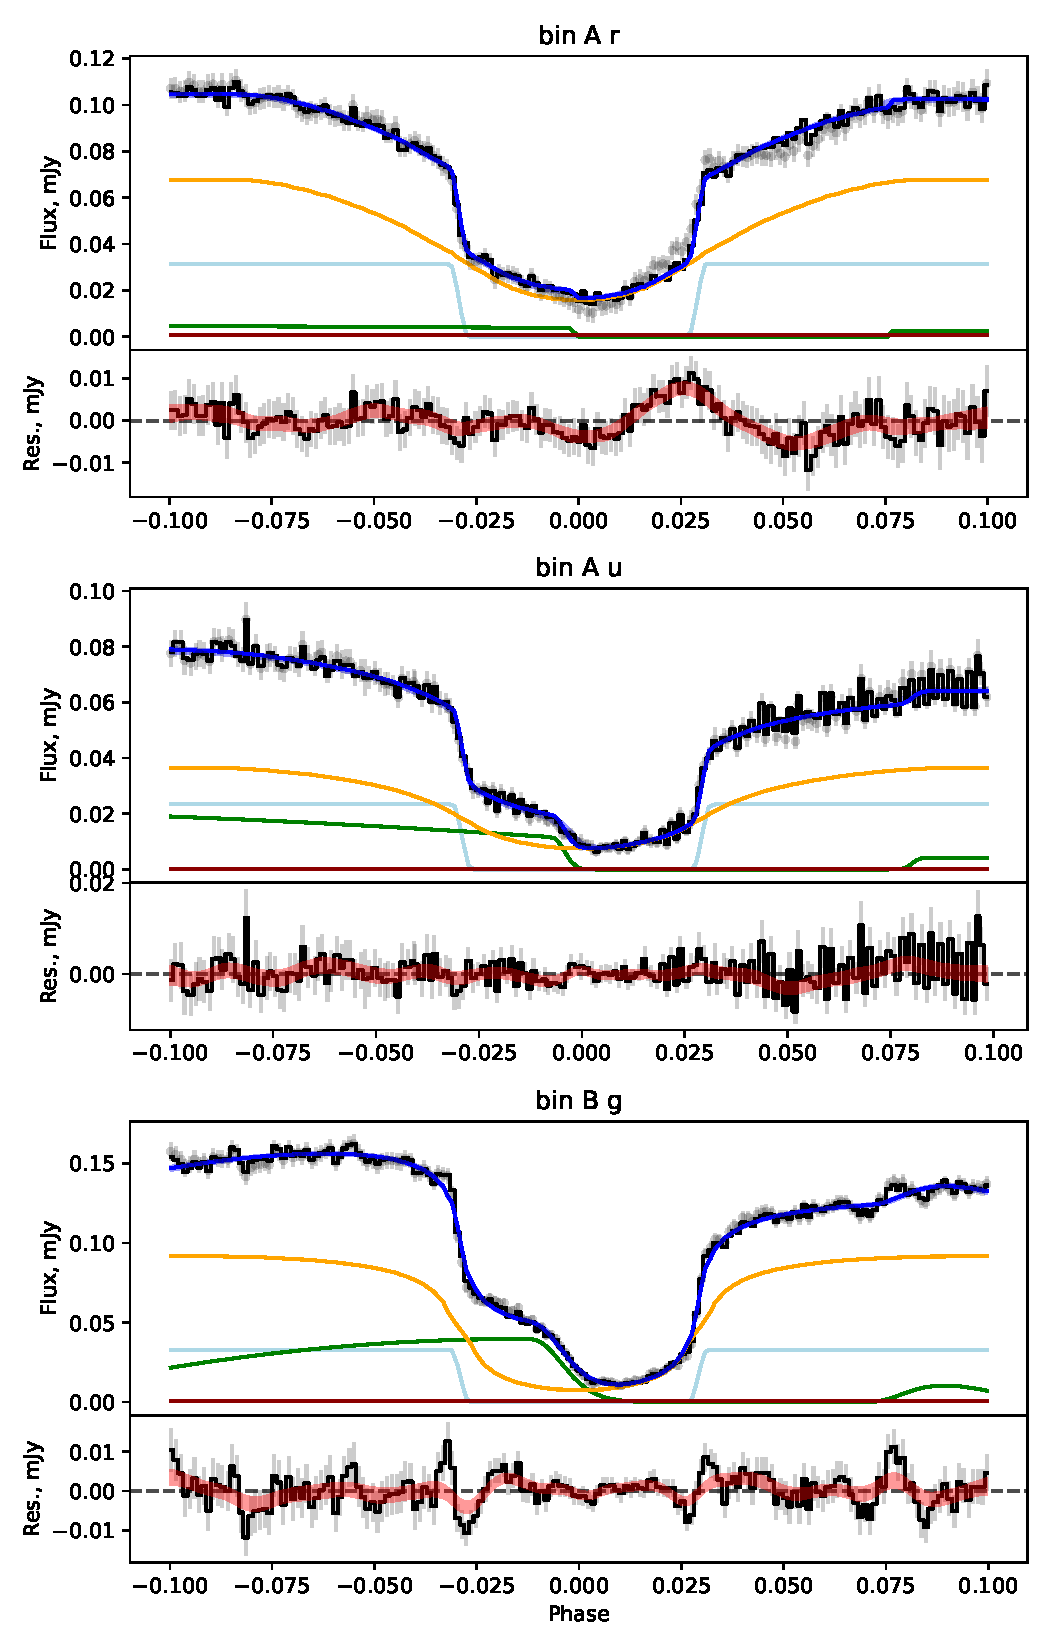
\includegraphics[width=\textwidth]{figures/results/SDSS1524/SDSS1524_3.pdf}
    \caption{SDSS J1524 lightcurve models (cont.)}
    \label{fig:SDSS1524 all lightcurves cont 2}
\end{figure}
\begin{figure}
    \centering
    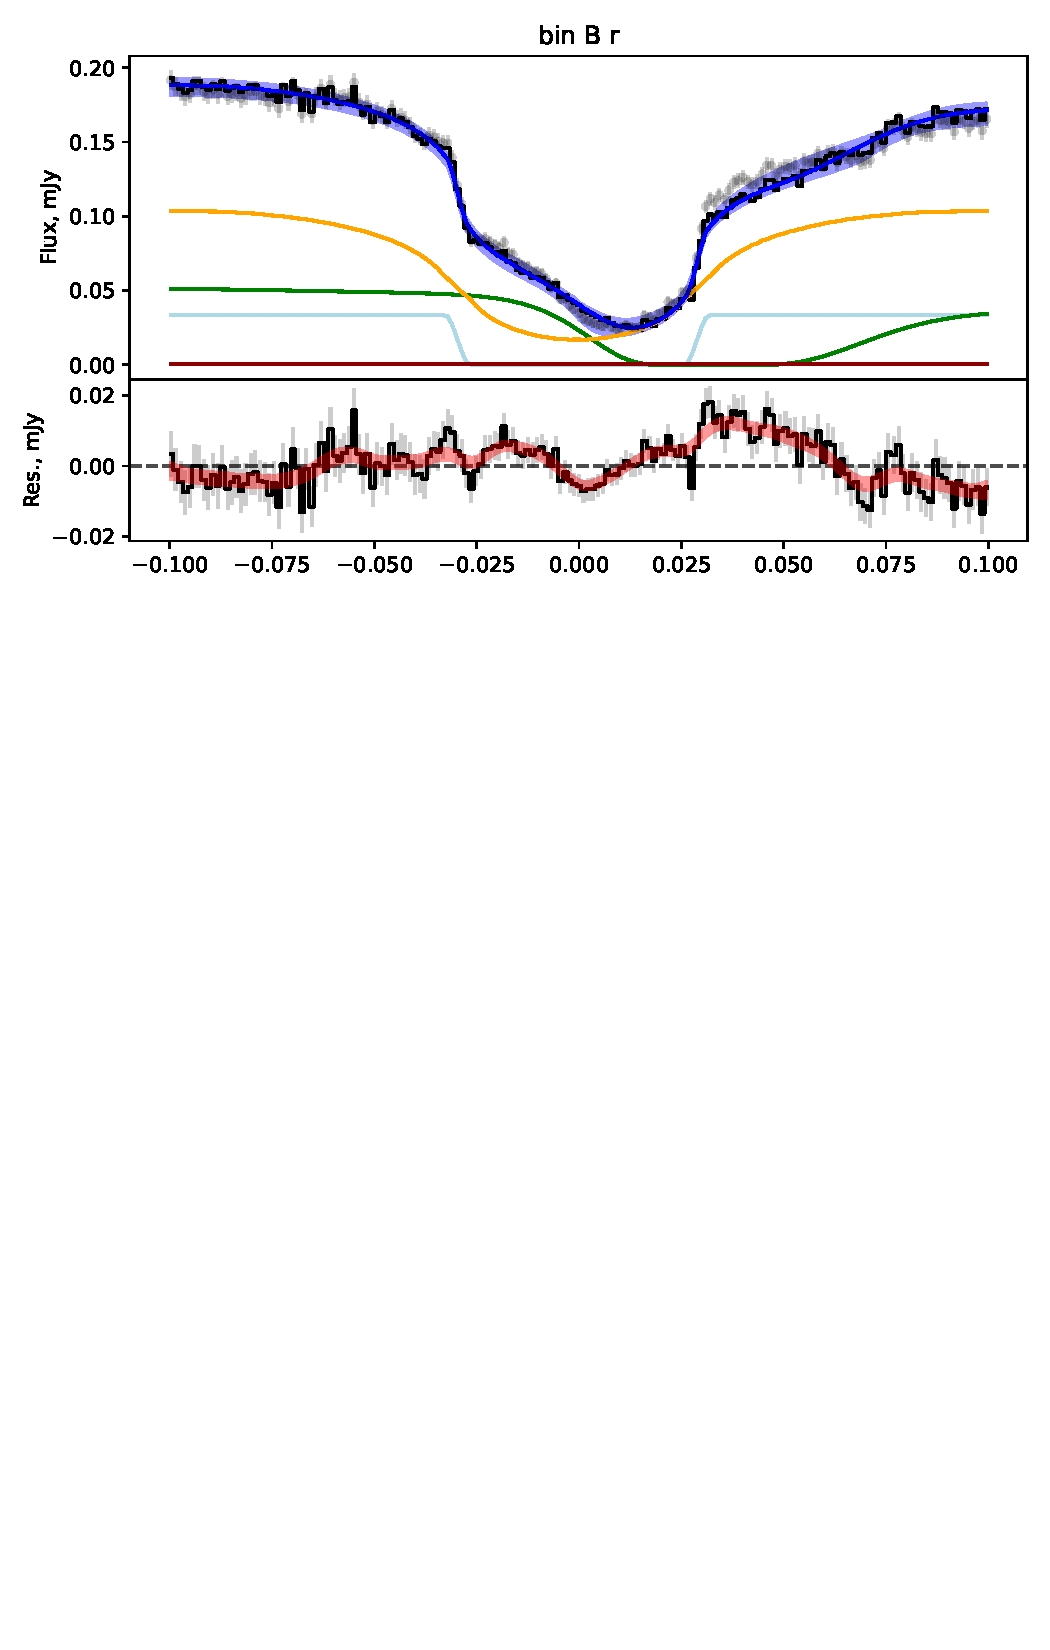
\includegraphics[width=\textwidth]{figures/results/SDSS1524/SDSS1524_4.pdf}
    \caption{SDSS J1524 lightcurve models (cont.)}
    \label{fig:SDSS1524 all lightcurves cont 3}
\end{figure}


\section{White dwarf flux distributions, compared to cooling tracks}
\label{appendix:white dwarf fluxes}

\begin{figure}
    \centering
    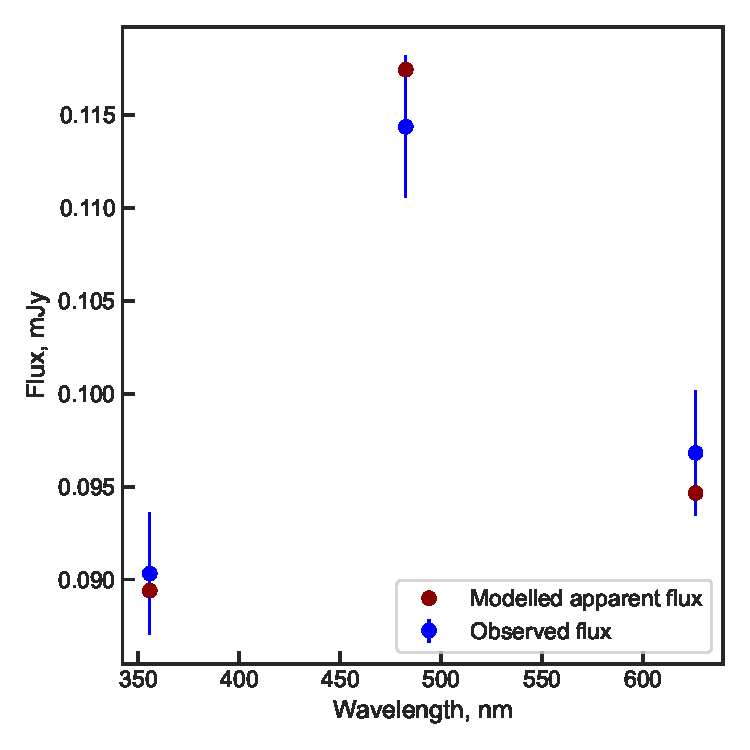
\includegraphics[width=\textwidth]{figures/results/ASASSN-14hq/fluxplot.pdf}
    \caption{ASASSN-14hq observed white dwarf fluxes, compared to the best-fit model atmosphere.}
    \label{fig:ASASSN-14hq flux plot}
\end{figure}

\begin{figure}
    \centering
    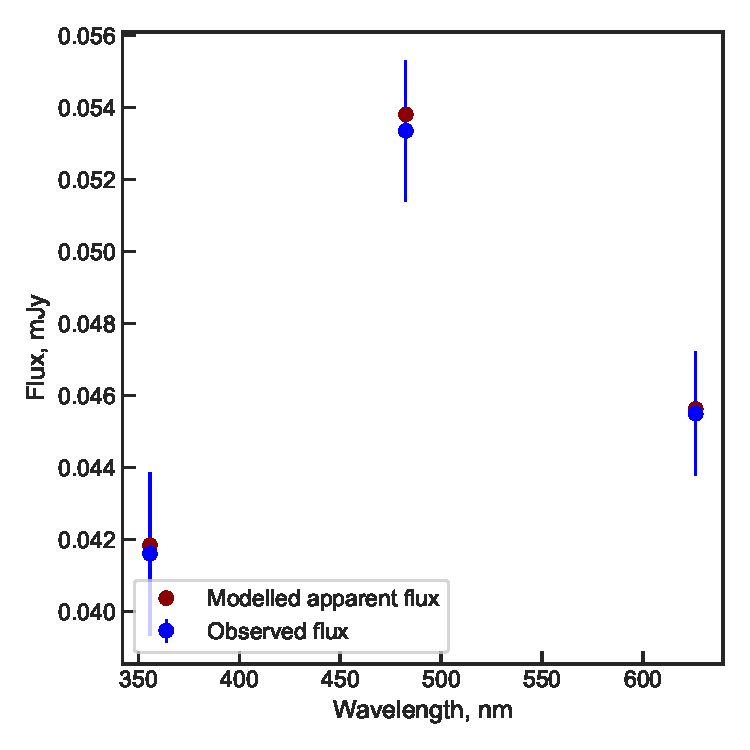
\includegraphics[width=\textwidth]{figures/results/ASASSN-14kb/fluxplot.pdf}
    \caption{ASASSN-14kb observed white dwarf fluxes, compared to the best-fit model atmosphere.}
    \label{fig:ASASSN-14kb flux plot}
\end{figure}

\begin{figure}
    \centering
    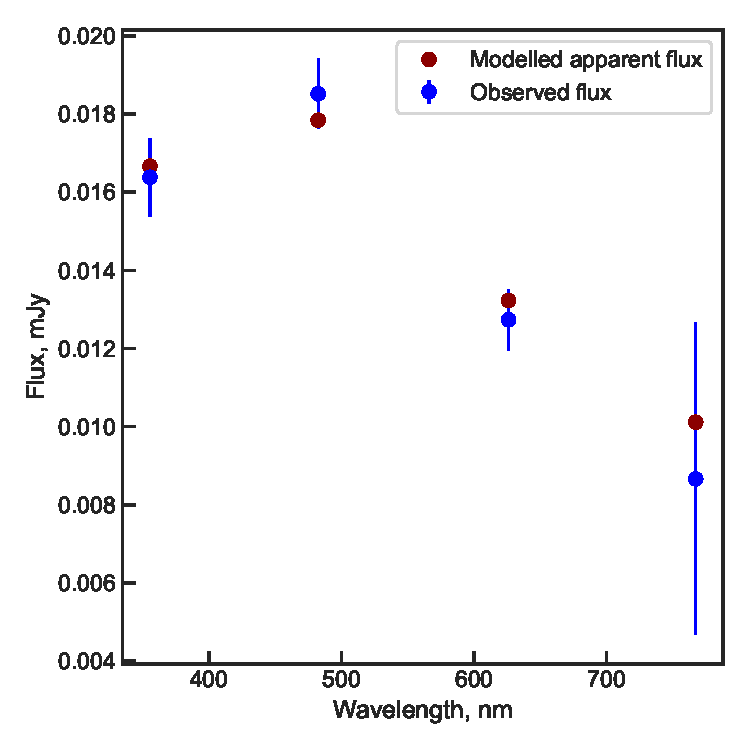
\includegraphics[width=\textwidth]{figures/results/ASASSN-15pb/fluxplot.pdf}
    \caption{ASASSN-15pb observed white dwarf fluxes, compared to the best-fit model atmosphere.}
    \label{fig:ASASSN-15pb flux plot}
\end{figure}

\begin{figure}
    \centering
    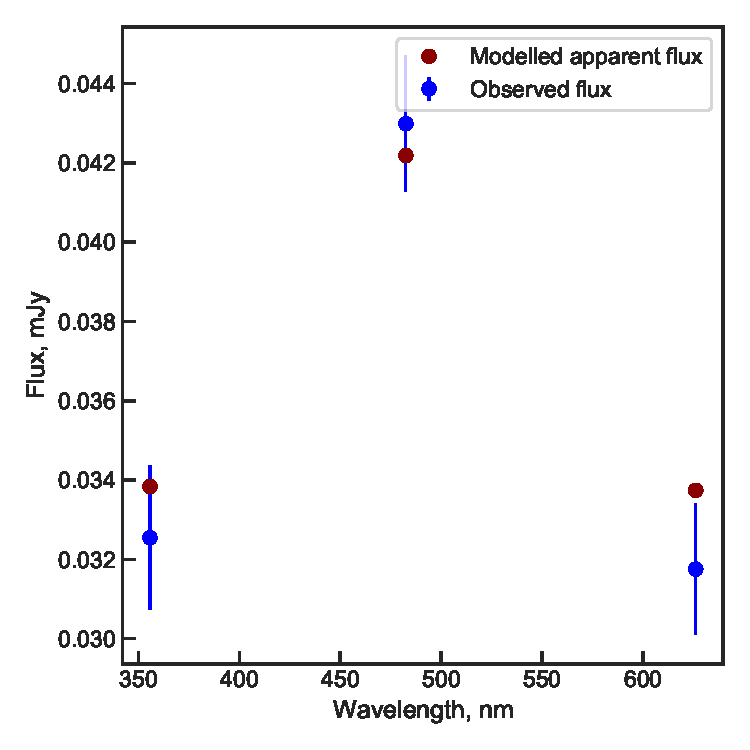
\includegraphics[width=\textwidth]{figures/results/ASASSN-17fo/fluxplot.pdf}
    \caption{ASASSN-17fo observed white dwarf fluxes, compared to the best-fit model atmosphere.}
    \label{fig:ASASSN-17fo flux plot}
\end{figure}

\begin{figure}
    \centering
    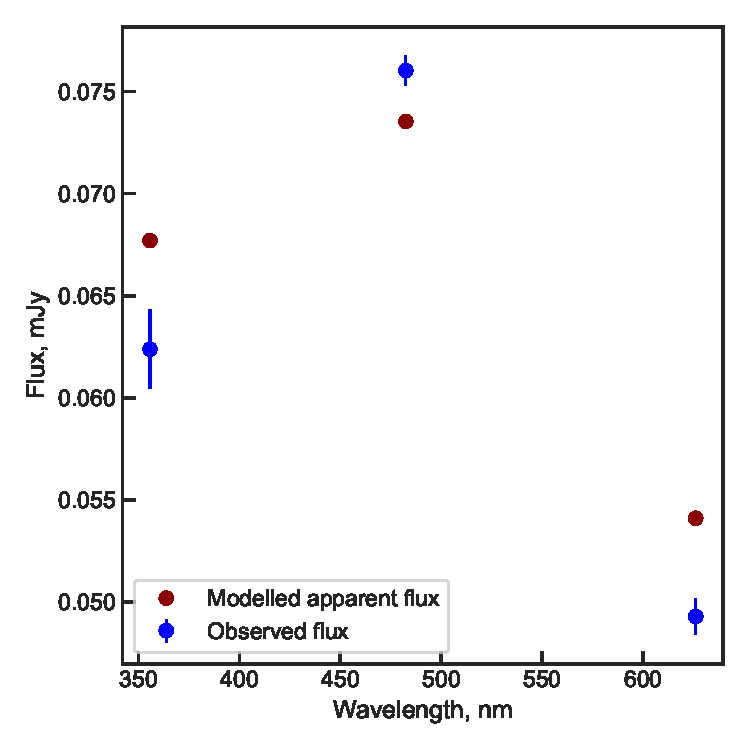
\includegraphics[width=\textwidth]{figures/results/AYFor/fluxplot.pdf}
    \caption{AY For observed white dwarf fluxes, compared to the best-fit model atmosphere.}
    \label{fig:AYFor flux plot}
\end{figure}

\begin{figure}
    \centering
    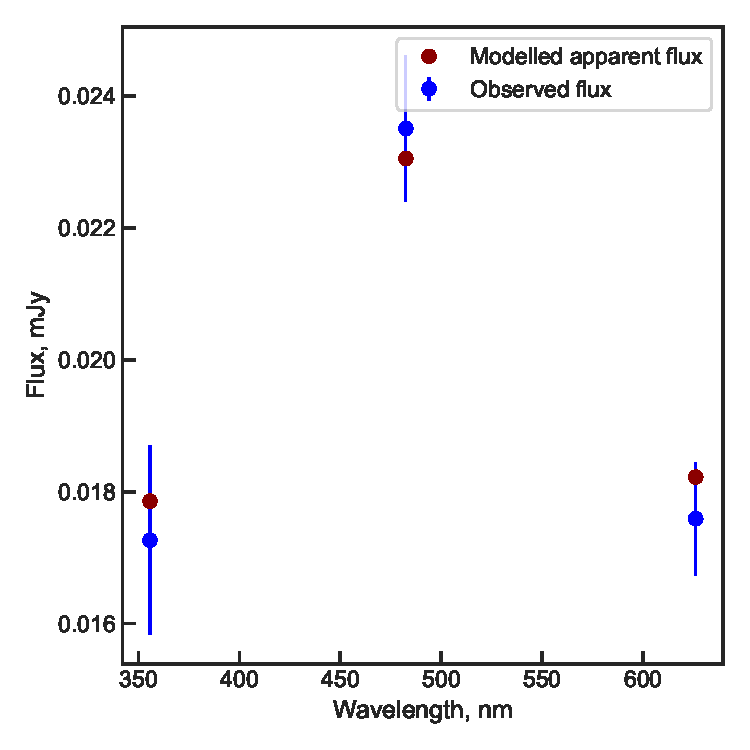
\includegraphics[width=\textwidth]{figures/results/CSS090102/fluxplot.pdf}
    \caption{CSS090102 observed white dwarf fluxes, compared to the best-fit model atmosphere.}
    \label{fig:CSS090102 flux plot}
\end{figure}

\begin{figure}
    \centering
    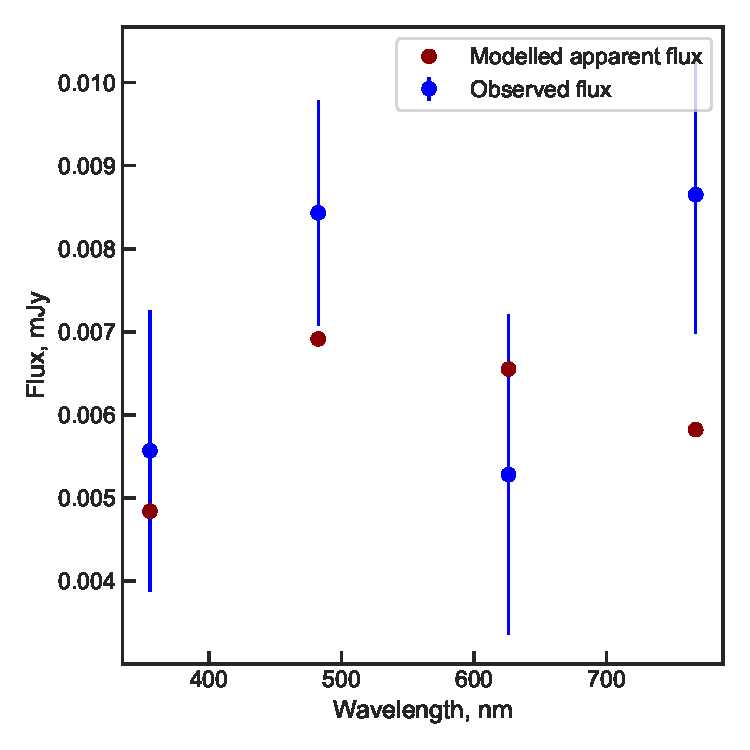
\includegraphics[width=\textwidth]{figures/results/CSS090419/fluxplot.pdf}
    \caption{CSS090419 observed white dwarf fluxes, compared to the best-fit model atmosphere.}
    \label{fig:CSS090419 flux plot}
\end{figure}

\begin{figure}
    \centering
    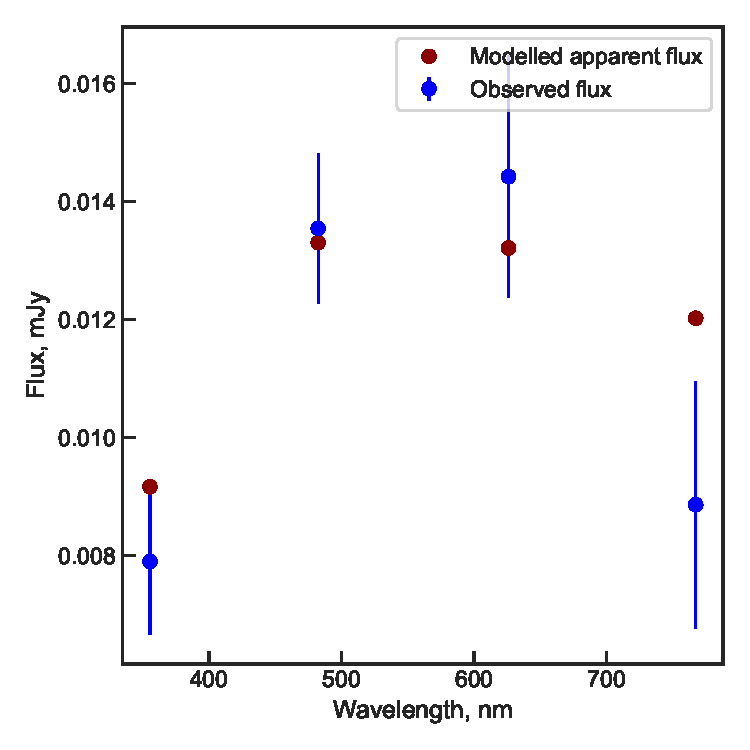
\includegraphics[width=\textwidth]{figures/results/CSS090622/fluxplot.pdf}
    \caption{CSS090622 observed white dwarf fluxes, compared to the best-fit model atmosphere.}
    \label{fig:CSS090622 flux plot}
\end{figure}

\begin{figure}
    \centering
    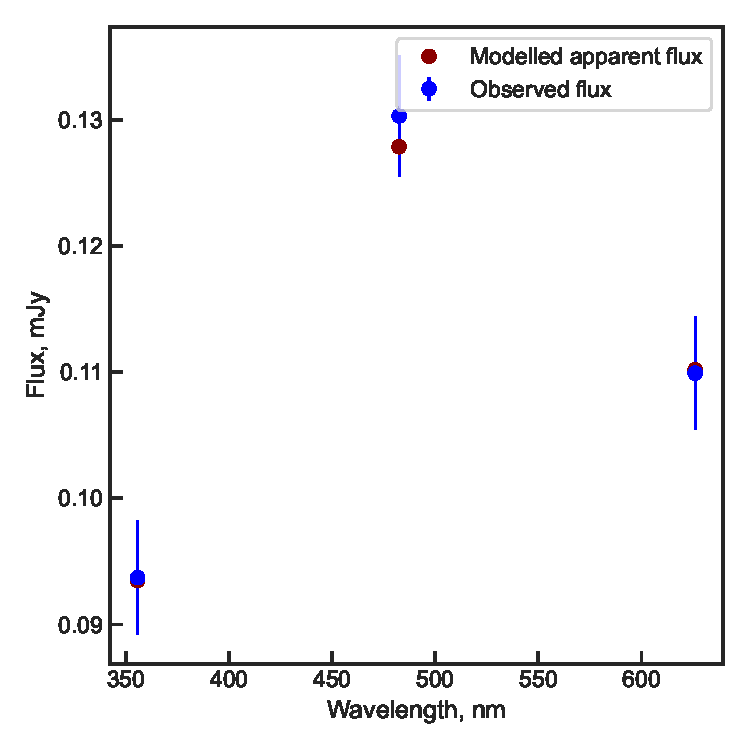
\includegraphics[width=\textwidth]{figures/results/OGLE82/fluxplot.pdf}
    \caption{OGLE82 observed white dwarf fluxes, compared to the best-fit model atmosphere.}
    \label{fig:OGLE82 flux plot}
\end{figure}

\begin{figure}
    \centering
    \includegraphics[width=\textwidth]{figures/results/SDSS0748/fluxplot.pdf}
    \caption{SDSS J0748 observed white dwarf fluxes, compared to the best-fit model atmosphere.}
    \label{fig:SDSS0748 flux plot}
\end{figure}

\begin{figure}
    \centering
    \includegraphics[width=\textwidth]{figures/results/MASOT0014/fluxplot.pdf}
    \caption{MAS0014 observed white dwarf fluxes, compared to the best-fit model atmosphere.}
    \label{fig:MAS0014 flux plot}
\end{figure}

\begin{figure}
    \centering
    \includegraphics[width=\textwidth]{figures/results/SDSS1524/fluxplot.pdf}
    \caption{SDSS1524 observed white dwarf fluxes, compared to the best-fit model atmosphere.}
    \label{fig:SDSS1524 flux plot}
\end{figure}


\section{Eclipse modelled CV sample}
\label{appendix:eclipse modelled CV data tables}

The following data are also available in machine-readable format upon reasonable request to the author.

\begin{landscape}

    \begin{table*}
        \centering
        \caption{The system parameters found for the 12 CVs analysed in Chapter~\ref{chpt:results:characterisation of 12 new CVs}. The reported parallax, $\pi$, is the posterior distribution from fitting the white dwarf fluxes, c.f.~\S\ref{sect:modelling:fitting white dwarf colours}.}
        \label{table:12 new cvs:system_parameters}
        \begin{tabular}{lccccc}
            \hline \\
            ~                          & \textbf{ASASSN-14hq}    & \textbf{ASASSN-14kb}     & \textbf{ASASSN-15pb}      & \textbf{ASASSN-17fo}      & \textbf{AY For}       \\
            \hline \hline \\
            $M_\mathrm{WD}/M_\odot$    & $0.67\pm0.01$           & $0.74\pm0.02$            & $0.72\pm0.03$             & $0.85\pm0.01$             & $0.78\pm0.02$         \\
            $R_\mathrm{WD}/R_\odot$    & $0.0119\pm0.0001$       & $0.0113\pm0.0002$        & $0.0115\pm0.0005$         & $0.0099\pm0.0001$         & $0.0106\pm0.0003$ \\
            $M_\mathrm{donor}/M_\odot$ & $0.097\pm0.002$         & $0.134\pm0.003$          & $0.148\pm0.008$           & $0.109\pm0.002$           & $0.106\pm0.006$ \\
            $R_\mathrm{donor}/R_\odot$ & $0.157\pm0.001$         & $0.164\pm0.001$          & $0.210\pm0.004$           & $0.1436\pm0.0007$         & $0.162\pm0.003$ \\
            $q$                        & $0.145\pm0.002$         & $0.182\pm0.002$          & $0.206\pm0.004$           & $0.1267\pm0.0005$         & $0.136\pm0.004$ \\
            \hline
            $P$, hours                 & $1.78384800(7)$         & $1.63453(1)$             & $2.23896(3)$              & $1.477147(2)$             & $1.790756(1)$ \\
            $a/R_\odot$,               & $0.681\pm0.004$         & $0.670\pm0.005$          & $0.824\pm0.014$           & $0.646\pm0.003$           & $0.717\pm0.007$ \\
            $i, ^\circ$                & $80.35\pm0.06$          & $84.4\pm0.1$             & $79.4\pm0.1$              & $84.23\pm0.03$            & $84.0\pm0.2$ \\
            $K_\mathrm{WD}$, km/s      & $58.0\pm0.9$            & $76.2\pm1$               & $75\pm2$                  & $60.2\pm0.4$              & $57.8\pm2.0$ \\
            $K_\mathrm{donor}$, km/s   & $399\pm2$               & $419\pm3$                & $364\pm6$                 & $468\pm2$                 & $425\pm4$ \\
            \hline
            $\pi$, mas                 & $3.40\pm0.07$           & $2.78\pm0.11$            & $1.0\pm0.2$               & $1.79\pm0.36$             & $2.12\pm0.16$ \\
            $T_{\rm eff}$, K           & $14819\pm800$           & $17700\pm1000$           & $19200\pm1600$            & $14800\pm600$             & $18100\pm500$ \\
            $\log(g), {\rm cgs}$       & $8.11\pm0.02$           & $8.21\pm0.03$            & $8.17\pm0.06$             & $8.37\pm0.02$             & $8.28\pm0.04$ \\
            \hline
            \hline
        \end{tabular}
    \end{table*}

    \begin{table*}
        \centering
        \caption{Table~\ref{table:12 new cvs:system_parameters}, continued.}
        \label{table:12 new cvs:system_parameters cont 1}
        \begin{tabular}{lccccc}
            \hline \\
            ~                          & \textbf{CSS090102}     & \textbf{CSS090419}    & \textbf{CSS090622}    & \textbf{OGLE82}   & \textbf{SDSS J0748} \\
            \hline \hline \\
            $M_\mathrm{WD}/M_\odot$    & $0.62\pm0.03$          & $0.59\pm0.08$         & $0.67\pm0.06$         & $0.83\pm0.01$     & $0.68\pm0.02$ \\
            $R_\mathrm{WD}/R_\odot$    & $0.0126\pm0.0004$      & $0.0122\pm0.0009$     & $0.0112\pm0.0007$     & $0.0099\pm0.0002$ & $0.0121\pm0.0004$ \\
            $M_\mathrm{donor}/M_\odot$ & $0.060\pm0.003$        & $0.087\pm0.011$       & $0.104\pm0.009$       & $0.131\pm0.004$   & $0.066\pm0.004$ \\
            $R_\mathrm{donor}/R_\odot$ & $0.119\pm0.002$        & $0.152\pm0.007$       & $0.155\pm0.005$       & $0.170\pm0.002$   & $0.117\pm0.002$ \\
            $q$                        & $0.094\pm0.002$        & $0.146\pm0.003$       & $0.159\pm0.008$       & $0.157\pm0.002$   & $0.095\pm0.004$ \\
            \hline
            $P$, hours                 & $1.49723786(5)$        & $1.81062621(6)$       & $1.702302(6)$         & $1.7263398(6)$    & $1.39947(1)$ \\
            $a/R_\odot$,               & $0.582\pm0.008$        & $0.660\pm0.030$       & $0.661\pm0.020$       & $0.720\pm0.006$   & $0.575\pm0.007$ \\
            $i, ^\circ$                & $88.7\pm0.6$           & $80.9\pm0.1$          & $88.2\pm0.6$          & $83.9\pm0.1$      & $81.7\pm0.2$ \\
            $K_\mathrm{WD}$, km/s      & $40.9\pm1.2$           & $56.0\pm2.7$          & $63.7\pm2.5$          & $68.5\pm1.0$      & $42.2\pm1.8$ \\
            $K_\mathrm{donor}$, km/s   & $431\pm6$              & $381\pm16$            & $408\pm12$            & $435\pm3$         & $450\pm5$ \\
            \hline
            $\pi$, mas                 & $1.41\pm0.30$          & $1.42\pm0.69$         & $2.02\pm0.27$         & $3.82\pm0.12$     & $1.83\pm0.14$ \\
            $T_{\rm eff}$, K           & $14800\pm1200$         & $18200\pm9000$        & $9800\pm1500$         & $18000\pm4000$    & $22500\pm3000$ \\
            $\log(g), {\rm cgs}$       & $8.00\pm0.33$          & $8.04\pm0.12$         & $8.16\pm0.08$         & $8.37\pm0.03$     & $8.11\pm0.03$ \\
            \hline
            \hline
        \end{tabular}
    \end{table*}

    \begin{table*}
        \centering
        \caption{Table~\ref{table:12 new cvs:system_parameters}, continued.}
        \label{table:12 new cvs:system_parameters cont 2}
        \begin{tabular}{lcc}
            \hline \\
            ~                          & \textbf{MASOT0014}     & \textbf{SDSS J1524} \\
            \hline \hline \\
            $M_\mathrm{WD}/M_\odot$    & $0.86\pm0.03$          & $0.80\pm0.04$ \\
            $R_\mathrm{WD}/R_\odot$    & $0.0097\pm0.0003$      & $0.0103\pm0.0005$ \\
            $M_\mathrm{donor}/M_\odot$ & $0.122\pm0.007$        & $0.074\pm0.008$ \\
            $R_\mathrm{donor}/R_\odot$ & $0.165\pm0.003$        & $0.132\pm0.005$ \\
            $q$                        & $0.142\pm0.004$        & $0.093\pm0.007$ \\
            \hline
            $P$, hours                 & $1.7167077(5)$         & $1.56764953(2)$ \\
            $a/R_\odot$,               & $0.722\pm0.008$        & $0.652\pm0.01197$ \\
            $i, ^\circ$                & $84.8\pm0.3$           & $86.7\pm1.1$ \\
            $K_\mathrm{WD}$, km/s      & $63.2\pm2.0$           & $42.9\pm3.4$ \\
            $K_\mathrm{donor}$, km/s   & $445\pm5$              & $461\pm7$ \\
            \hline
            $\pi$, mas                 & $2.42\pm0.11$          & $1.92\pm0.19$ \\
            $T_{\rm eff}$, K           & $17300\pm1000$         & $12500\pm1100$ \\
            $\log(g), {\rm cgs}$       & $8.37\pm0.04$          & $8.32\pm0.06$ \\
            \hline
            \hline
        \end{tabular}
    \end{table*}


    \begin{table*}
        \centering
        \caption{The system parameters found for the three CVs with peculiar white dwarf colours. Here, the reported $\pi$ is the posterior distribution from fitting the white dwarf fluxes, c.f. \S\ref{sect:modelling:fitting white dwarf colours}.}
        \label{table:three white dwarfs:system_parameters}
        \begin{tabular}{lccc}
            \hline \\
            ~                          & \textbf{ASASSN-16kr}    & \textbf{ASASSN-17jf}  & \textbf{SSSJ0522-3505} \\
            \hline \hline \\
            $M_\mathrm{WD}/M_\odot$    & $0.952\pm0.018$         & $0.669\pm0.031$        & $0.760\pm0.023$ \\
            $R_\mathrm{WD}/R_\odot$    & $0.0083\pm0.0002$       & $0.0120\pm0.0004$      & $0.0112\pm0.0003$ \\
            $M_\mathrm{donor}/M_\odot$ & $0.042\pm0.001$         & $0.060\pm0.008$        & $0.042\pm0.004$ \\
            $R_\mathrm{donor}/R_\odot$ & $0.105\pm0.002$         & $0.112\pm0.004$        & $0.105\pm0.004$ \\
            $q$                        & $0.044\pm0.002$         & $0.085\pm0.006$        & $0.055\pm0.003$ \\
            \hline
            $P$, hours                 & $1.470862368(2)$        & $1.36297(2)$           & $1.492642(2)$ \\
            $a/R_\odot$,               & $0.653\pm0.005$         & $0.567\pm0.009$        & $0.614\pm0.007$  \\
            $i, ^\circ$                & $86.4\pm0.4$            & $83.7\pm0.5$           & $83.8\pm0.3$  \\
            $K_\mathrm{WD}$, km/s      & $22.7\pm1.5$            & $39.5\pm4.2$           & $26.0\pm1.8$  \\
            $K_\mathrm{donor}$, km/s   & $515\pm3$               & $462\pm5$              & $470\pm4$  \\
            \hline
            $\pi$, mas                 & $6.58\pm0.22$           & $2.09\pm0.19$          & $1.81\pm0.11$  \\
            $T_{\rm eff}$, kK          & $10-12$                 & $8-13$                 & $\sim25$  \\
            $\log(g), {\rm cgs}$       & $8.55\pm0.03$           & $8.15\pm0.05$          & $8.22\pm0.04$  \\
            \hline
            \hline
        \end{tabular}
    \end{table*}


    \begin{table*}
        \caption{System parameters for 15 eclipsing systems from \citet{McAllister2019}.}
        \label{table:mcallister system params}
        \begin{tabular}{lcccccc}
            \hline
            ~                           & \textbf{CSS080623}                & \textbf{CSS110113}        & \textbf{CTCV 1300}                & \textbf{DV UMa}               & \textbf{GY Cnc}                   & \textbf{IY UMa}                   \\
            \hline
            \hline
            $M_{\rm wd}/M_{\odot}$      & $0.710\pm0.019$                   & $1.00\,^{+0.04}_{-0.01}$  & $0.717\pm0.017$                   & $1.09\pm0.03$                 & $0.881\pm0.016$                   & $0.955\,^{+0.013}_{-0.028}$       \\
            $R_{\rm wd}/R_{\odot}$      & $0.0117\,^{+0.0001}_{-0.0004}$    & $0.0080\pm0.0003$         & $0.01133\pm0.00021$               & $0.0072\pm0.0004$             & $0.00976\,^{+0.00021}_{-0.00018}$ & $0.0087\,^{+0.0003}_{-0.0001}$    \\
            $M_{\rm donor}/M_{\odot}$   & $0.081\pm0.005$                   & $0.105\pm0.007$           & $0.166\,^{+0.006}_{-0.003}$       & $0.187\,^{+0.003}_{-0.012}$   & $0.394\,^{+0.016}_{-0.022}$       & $0.141\pm0.007$                   \\
            $R_{\rm donor}/R_{\odot}$   & $0.1275\pm0.0024$                 & $0.149\pm0.003$           & $0.2111\,^{+0.0025}_{-0.0014}$    & $0.215\,^{+0.001}_{-0.005}$   & $0.446\,^{+0.006}_{-0.009}$       & $0.1770\pm0.0028$                 \\
            $q$                         & $0.114\pm0.005$                   & $0.105\pm0.006$           & $0.233\pm0.004$                   & $0.172\,^{+0.002}_{-0.007}$   & $0.448\,^{+0.014}_{-0.021}$       & $0.146\,^{+0.009}_{-0.001}$       \\
            \hline
            $P$ (hours)                 & $1.429895304(72)$                 & $1.585220897(3)$          & $2.134576795(41)$                 & $2.060463139(17)$             & $4.210617576(144)$                & $1.773814276(5)$                  \\
            $a/R_{\odot}$               & $0.593\pm0.005$                   & $0.711\,^{+0.009}_{-0.003}$   & $0.805\pm0.007$               & $0.889\,^{+0.006}_{-0.012}$   & $1.429\pm0.012$                   & $0.765\,^{+0.004}_{-0.009}$       \\
            $i, ^\circ$                 & $80.76\pm0.19$                    & $79.94\pm0.19$                & $86.9\,^{+0.5}_{-0.2}$        & $83.29\,^{+0.29}_{-0.10}$     & $77.06\,^{+0.29}_{-0.18}$         & $84.9\,^{+0.1}_{-0.5}$            \\
            $K_{\rm wd}$ km/s           & $50.8\pm2.3$                      & $51.1\,^{+2.9}_{-2.4}$        & $86.4\pm1.4$                  & $76.1\,^{+0.9}_{-2.9}$        & $125\pm4$                         & $66\,^{+4}_{-1}$                  \\
            $K_{\rm donor}$ km/s        & $449\,^{+1}_{-6}$                 & $487\pm3$                     & $371\pm3$                     & $444\pm4$                     & $278.0\pm2.4$                     & $453\pm3$                         \\
            \hline
            $d$, pc                     & $550\pm60$                        & $430\pm60$                & $340\pm40$                        & $380\pm40$                    & $320\pm30$                        & --                                \\
            $T_{\rm eff} (K)$           & $15500\pm1700$                    & $14500\pm2200$            & $11000\pm1000$                    & $17400\pm1900$                & $25900\pm2300$                    & --                                \\
            $\log(g), {\rm cgs}$        & $8.15\,^{+0.01}_{-0.04}$          & $8.63\pm0.03$             & $8.186\pm0.019$                   & $8.77\pm0.04$                 & $8.40\pm0.019$                    & $8.54\pm0.03$                     \\
            \hline \hline
        \end{tabular}
    \end{table*}

    \begin{table*}
        \caption{Table~\ref{table:mcallister system params}, continued.}
        \label{table:mcallister system params cont 1}
        \begin{tabular}{lcccccc}
            \hline
            ~                           & \textbf{OY Car}                   & \textbf{SDSS 0901}                    & \textbf{SDSS 1006}            & \textbf{SDSS 1152}            & \textbf{SDSS 1501}                                        & \textbf{SSS100615}                \\
            \hline
            \hline
            $M_{\rm wd}/M_{\odot}$      & $0.882\,^{+0.011}_{-0.015}$       & $0.752\,^{+0.024}_{-0.018}$           & $0.82\pm0.11$                 & $0.62\pm0.04$                 & $0.723\,^{+0.017}_{-0.013}$                               & $0.88\pm0.03$                     \\
            $R_{\rm wd}/R_{\odot}$      & $0.00957\,^{+0.00018}_{-0.00012}$ & $0.01105\,^{+0.00022}_{-0.00029}$     & $0.0102\pm0.0013$             & $0.0129\pm0.0006$             & $0.01142\,^{+0.00016}_{-0.00022}$                         & $0.0095\pm0.0003$                 \\
            $M_{\rm donor}/M_{\odot}$   & $0.093\,^{+0.004}_{-0.001}$       & $0.138\pm0.007$                       & $0.37\pm0.06$                 & $0.094\,^{+0.016}_{-0.009}$   & $0.061\pm0.004$                                           & $0.083\pm0.005$                   \\
            $R_{\rm donor}/R_{\odot}$   & $0.1388\,^{+0.0018}_{-0.0003}$    & $0.182\pm0.003$                       & $0.457\,^{+0.022}_{-0.026}$   & $0.147\pm0.006$               & $0.1129\,^{+0.0025}_{-0.0016}$                            & $0.1276\,^{+0.0028}_{-0.0024}$    \\
            $q$                         & $0.1065\,^{+0.0009}_{-0.0029}$    & $0.182\,^{+0.009}_{-0.004}$           & $0.46\pm0.03$                 & $0.153\,^{+0.015}_{-0.011}$   & $0.084\pm0.004$                                           & $0.095\pm0.004$                   \\
            \hline
            $P$ (hours)                  & $1.514902211(6)$                  & $1.869132770(12)$                     & $4.461914568(312)$            & $1.625992862(7)$              & $1.364190385(5)$                                          & $1.4089080(96)$                   \\
            $a/R_{\odot}$               & $0.662\pm0.003$                   & $0.739\pm0.007$                       & $1.46\pm0.07$                 & $0.627\pm0.014$               & $0.574\pm0.004$                                           & $0.628\pm0.007$                   \\
            $i, ^\circ$                 & $83.27\,^{+0.10}_{-0.13}$         & $81.4\,^{+0.1}_{-0.3}$                & $83.1\,^{+1.2}_{-0.7}$        & $82.6\pm0.5$                  & $83.89\,^{+0.20}_{-0.27}$                                 & $85.1\pm0.3$                      \\
            $K_{\rm wd}$ km/s           & $50.4\pm0.9$                      & $73\pm3$                              & $124\pm9$                     & $62\pm5$                      & $39.5\,^{+2.2}_{-1.3}$                                    & $46.5\,^{+2.2}_{-1.7}$            \\
            $K_{\rm donor}$ km/s        & $475.9\pm2.1$                     & $401\pm3$                             & $270\pm13$                    & $402\pm7$                     & $468\pm3$                                                 & $493\pm5$                         \\
            \hline
            $d$, pc                     & $90\pm5$                          & $600\pm70$                            & --                            & $610\pm80$                    & $^{400\,\pm\,30\,(2004)}_{338\,\pm\,21\,(2012)}$          & $350\pm30$                        \\
            $T_{\rm eff} (K)$           & $18600\,^{+2800}_{-1600}$         & $14900\pm2000$                        & --                            & $15900\pm2000$                & $^{13400\,\pm\,1100\,(2004)}_{14900\,\pm\,1000\,(2012)}$  & $13600\pm1500$                    \\
            $\log(g), {\rm cgs}$        & $8.422\,^{+0.017}_{-0.013}$       & $8.228\,^{+0.022}_{-0.025}$           & $8.33\pm0.13$                 & $8.01\pm0.05$                 & $8.182\,^{+0.016}_{-0.019}$                               & $8.43\pm0.03$                     \\
            \hline \hline
        \end{tabular}
    \end{table*}

    \begin{table*}
        \caption{Table~\ref{table:mcallister system params}, continued.}
        \label{table:mcallister system params cont 2}
        \begin{tabular}{lccc}
        \hline
        ~                               & \textbf{SSS130413}                & \textbf{V713 Cep}                 & \textbf{Z Cha}            \\
        \hline
        \hline
        $M_{\rm wd}/M_{\odot}$          & $0.84\pm0.03$                     & $0.703\,^{+0.012}_{-0.015}$       & $0.803\pm0.014$           \\
        $R_{\rm wd}/R_{\odot}$          & $0.0102\,^{+0.0006}_{-0.0002}$    & $0.01173\,^{+0.00020}_{-0.00015}$ & $0.01046\pm0.00017$       \\
        $M_{\rm donor}/M_{\odot}$       & $0.140\,^{+0.012}_{-0.008}$       & $0.176\,^{+0.007}_{-0.018}$       & $0.152\pm0.005$           \\
        $R_{\rm donor}/R_{\odot}$       & $0.163\pm0.004$                   & $0.208\,^{+0.002}_{-0.005}$       & $0.1820\pm0.0020$         \\
        $q$                             & $0.169\,^{+0.011}_{-0.006}$       & $0.246\,^{+0.006}_{-0.014}$       & $0.189\pm0.004$           \\
        \hline
        $P$ (hours)                      & $1.578462967(29)$                 & $2.050044192(29)$                 & $1.787982314(7)$          \\
        $a/R_{\odot}$                   & $0.680\,^{+0.007}_{-0.011}$       & $0.781\pm0.006$                   & $0.734\pm0.005$           \\
        $i, ^\circ$                     & $82.5\pm0.3$                      & $81.7\pm0.3$                      & $80.44\pm0.11$            \\
        $K_{\rm wd}$ km/s               & $75\pm4$                          & $91\,^{+2}_{-5}$                  & $78.4\,^{+1.4}_{-1.8}$    \\
        $K_{\rm donor}$ km/s            & $443\,^{+3}_{-7}$                 & $367.6\,^{+2.6}_{-2.3}$           & $413.2\,^{+2.5}_{-2.0}$   \\
        \hline
        $d$, pc                         & $240\pm40$                        & $320\pm30$                        & $103\pm6$                 \\
        $T_{\rm eff} (K)$               & $24000\pm3000$                    & $17000\,^{+6000}_{-3000}$         & $16300\pm1400$            \\
        $\log(g), {\rm cgs}$            & $8.35\pm0.04$                     & $8.147\,^{+0.017}_{-0.014}$       & $8.304\pm0.016$           \\
        \end{tabular}
        \end{table*}


        \begin{table*}
            \centering
            \caption{System parameters derived by \citet{Savoury2011}.}
            \label{table:savoury system params}
            \begin{tabular}{lcccc}
                \hline
                ~                           & {\bf CTCV J1300-3052} & {\bf CTCV J2354-4700} & {\bf SDSS J1152+4049} & {\bf OU Vir}      \\
                \hline
                \hline
                $M_{\rm wd}/M_{\odot}$      & $0.736\pm0.014$       & $0.935\pm0.031$       & $0.560\pm0.028$   & $0.703\pm0.012$       \\
                $R_{\rm wd}/R_{\odot}$      & $0.01111\pm0.00018$   & $0.0089\pm0.0003$     & $0.0135\pm0.0004$ & $0.01191\pm0.00017$   \\
                $M_{\rm donor}/M_{\odot}$   & $0.177\pm0.021$       & $0.101\pm0.003$       & $0.087\pm0.006$   & $0.1157\pm0.0022$     \\
                $R_{\rm donor}/R_{\odot}$   & $0.215\pm0.008$       & $0.1463\pm0.0016$     & $0.142\pm0.003$   & $0.1634\pm0.0010$     \\
                $q$                         & $0.240\pm0.021$       & $0.1097\pm0.0008$     & $0.155\pm0.006$   & $0.1641\pm0.0013$     \\
                \hline
                $P$ (mins)                  & $128.0746325(14)$     & $94.3923889(14)$      & $97.518753(4)$    & $104.696803(7)$       \\
                $a/R_{\odot}$               & $0.813\pm0.011$       & $0.692\pm0.008$       & $0.606\pm0.010$   & $0.686\pm0.004$       \\
                $i, ^\circ$                 & $86.3\pm1.1$          & $89.26\pm0.28$        & $82.38\pm0.23$    & $79.60\pm0.04$        \\
                $K_{\rm wd}$ km/s           & $90\pm8$              & $51.9\pm0.6$          & $60\pm3$          &  $66.4\pm0.6$         \\
                $K_{\rm donor}$ km/s        & $372.2\pm2.5$         & $482\pm6$             & $387\pm6$         & $403.0\pm2.3$         \\
                \hline
                $d$, pc                     & $375\pm13$            & $674\pm19$            & $543\pm21$        & $570\pm70$            \\
                $T_{\rm eff} (K)$           & $11100\pm800$         & $14800\pm700$         & $12400\pm1400$    & $22300\pm2100$        \\
                $\log(g), {\rm cgs}$        & $8.21\pm0.02$         & $8.51\pm0.04$         & $7.93\pm0.05$     & $8.13\pm0.02$         \\
                \hline
                \hline
            \end{tabular}
        \end{table*}

        \begin{table*}
            \caption{Table~\ref{table:savoury system params}, continued}
            \label{table:savoury system params cont 1}
            \begin{tabular}{lccccc}
                \hline
                ~                           & {\bf SDSS 1035}       & {\bf DV UMa}          & {\bf XZ Eri}          & {\bf SDSS 1702}       & {\bf SDSS 1501}       \\
                \hline
                \hline
                $M_{\rm wd}/M_{\odot}$      & $0.835\pm0.009$       & $1.098\pm0.024$       & $0.769\pm0.017$       & $0.91\pm0.03$         & $0.767\pm0.027$       \\
                $R_{\rm wd}/R_{\odot}$      & $0.00991\pm0.00010$   & $0.00703\pm0.00028$   & $0.01081\pm0.00022$   & $0.0092\pm0.0004$     & $0.0107\pm0.0003$     \\
                $M_{\rm donor}/M_{\odot}$   & $0.0475\pm0.0012$     & $0.196\pm0.005$       & $0.091\pm0.004$       & $0.223\pm0.010$       & $0.077\pm0.010$       \\
                $R_{\rm donor}/R_{\odot}$   & $0.1047\pm0.0008$     & $0.2176\pm0.0018$     & $0.1350\pm0.0018$     & $0.252\pm0.004$       & $0.122\pm0.005$       \\
                $q$                         & $0.0571\pm0.0010$     & $0.1778\pm0.0022$     & $0.118\pm0.003$       & $0.248\pm0.005$       & $0.101\pm0.010$       \\
                \hline
                $P$ (mins)                  & $82.08965(29)$        & $123.6278190(20)$     & $88.069667(7)$        & $144.11821(13)$       & $81.85141771(28)$     \\
                $a/R_{\odot}$               & $0.5977\pm0.0022$     & $0.892\pm0.006$       & $0.621\pm0.005$       & $0.945\pm0.012$       & $0.588\pm0.008$       \\
                $i, ^\circ$                 & $83.98\pm0.08$        & $82.93\pm0.10$        & $80.02\pm0.12$        & $82.55\pm0.17$        & $82.8\pm0.5$          \\
                $K_{\rm wd}$ km/s           & $28.5\pm0.6$          & $78.9\pm1.0$          & $53.6\pm1.5$          & $94.0\pm2.2$          & $48\pm5$              \\
                $K_{\rm donor}$ km/s        & $499.3\pm1.5$         & $443\pm3$             & $452\pm3$             & $380\pm4$             & $470.5\pm3.2$         \\
                \hline
                $d$, pc                     & $174\pm12$            & $504\pm30$            & $371\pm19$            & $270\pm16$            & $306\pm21$            \\
                $T_{\rm eff} (K)$           & $10000\pm1100$        & $15500\pm2400$        & $15300\pm1900$        & $15200\pm1200$        & $10800\pm1500$        \\
                $\log(g), {\rm cgs}$        & $8.37\pm0.01$         & $8.78\pm0.04$         & $8.26\pm0.03$         & $8.47\pm0.05$         & $8.26\pm0.04$         \\
                \hline
                \hline
            \end{tabular}
        \end{table*}

        \begin{table*}
            \caption{Table~\ref{table:savoury system params}, continued}
            \label{table:savoury system params cont 2}
            \begin{tabular}{lccccc}
                \hline
                ~                           & {\bf SDSS 1507}       & {\bf SDSS 0903}       & {\bf SDSS 1227}       & {\bf SDSS 1433}       & {\bf SDSS 1502}       \\
                \hline
                \hline
                $M_{\rm wd}/M_{\odot}$      & $0.892\pm0.008$       & $0.872\pm0.011$       & $0.796\pm0.018$       & $0.865\pm0.005$       & $0.709\pm0.004$       \\
                $R_{\rm wd}/R_{\odot}$      & $0.00956\pm0.00013$   & $0.00947\pm0.00019$   & $0.01052\pm0.00022$   & $0.00962\pm0.00006$   & $0.01145\pm0.00005$   \\
                $M_{\rm donor}/M_{\odot}$   & $0.0575\pm0.0020$     & $0.099\pm0.004$       & $0.0889\pm0.0025$     & $0.0571\pm0.0007$     & $0.0781\pm0.0008$     \\
                $R_{\rm donor}/R_{\odot}$   & $0.0969\pm0.0011$     & $0.1358\pm0.0020$     & $0.1365\pm0.0013$     & $0.1074\pm0.0004$     & $0.1241\pm0.0003$     \\
                $q$                         & $0.0647\pm0.0018$     & $0.113\pm0.004$       & $0.1115\pm0.0016$     & $0.0661\pm0.0007$     & $0.1099\pm0.0007$     \\
                \hline
                $P$ (mins)                  & $66.61192(6)$         & $85.065902(13)$       & $90.661019(10)$       & $78.106657(3)$        & $84.82984(7)$         \\
                $a/R_{\odot}$               & $0.5329\pm0.0019$     & $0.632\pm0.003$       & $0.640\pm0.005$       & $0.5869\pm0.0012$     & $0.5844\pm0.0013$     \\
                $i, ^\circ$                 & $83.47\pm0.12$        & $82.09\pm0.19$        & $84.29\pm0.10$        & $84.36\pm0.05$        & $88.35\pm0.17$        \\
                $K_{\rm wd}$ km/s           & $35.1\pm1.0$          & $54.6\pm2.0$          & $51.3\pm0.8$          & $33.8\pm0.3$          & $50.4\pm0.4$          \\
                $K_{\rm donor}$ km/s        & $543.7\pm1.2$         & $481.7\pm1.9$         & $460\pm3$             & $511.1\pm0.9$         & $456.5\pm0.8$         \\
                \hline
                $d$, pc                     & $168\pm12$            & $299\pm14$            & $400\pm13$            & $226\pm12$            & $175\pm11$            \\
                $T_{\rm eff} (K)$           & $11300\pm1000$        & $13300\pm1700$        & $15900\pm1400$        & $12700\pm1500$        & $11800\pm1200$        \\
                $\log(g), {\rm cgs}$        & $8.45\pm0.01$         & $8.42\pm0.02$         & $8.29\pm0.02$         & $8.41\pm0.01$         & $8.17\pm0.01$         \\
                \hline
                \hline
            \end{tabular}
        \end{table*}


        \begin{table*}
            \centering
            \caption{System parameters from assorted other sources: \citet{mcallister2015} (M15), \citet{mcallister2017} (M17a), \citet{mcallister2017b} (M17b), \citet{copperwheat2010} (C10), \citet{shafter2003} (S03), }
            \label{table:supplementary systems}
            \begin{tabular}{lcccccc}
                \hline
                ~                           & \textbf{PHL 1445}         & \textbf{SDSS J1057+2759}  & \textbf{ASASSN-14ag}  & \textbf{IP Peg}       \\
                \hline \hline
                $M_\mathrm{WD}/M_\odot$     & $0.733\pm0.006$           & $0.800\pm0.015$           & $0.63\pm0.04$         & $1.16\pm0.02$         \\
                $R_\mathrm{WD}/R_\odot$     & $0.01122\pm0.00008$       & $0.01040\pm0.00017$       & $0.0126\pm0.0006$     & $0.0081\pm0.0013$     \\
                $M_\mathrm{donor}/M_\odot$  & $0.0637\pm0.0007$         & $0.0436\pm0.0020$         & $0.093\pm0.013$       & $0.55\pm0.04$         \\
                $R_\mathrm{donor}/R_\odot$  & $0.1092\pm0.0004$         & $0.1086\pm0.0017$         & $0.135\pm0.007$       & $0.46\pm0.02$         \\
                $q$                         & $0.08701\pm0.0005$        & $0.0546\pm0.0020$         & $0.149\pm0.016$       & $0.47\pm0.03$         \\
                \hline
                $P$, days                   & $0.0529848884(13)$        & $0.0627919557(6)$         & $0.060310665(9)$      & $0.1582061029(3)$     \\
                $a/R_\odot$,                & $0.550\pm0.011$           & $0.629\pm0.004$           & $0.583\pm0.015$       & $1.472\pm0.009$       \\
                $i, ^\circ$                 & $85.2\pm0.9$              & $85.74\pm0.21$            & $83.4\pm0.7$          & $83.81\pm0.45$        \\
                $K_\mathrm{WD}$, km/s       & $42\pm3$                  & $26.2\pm0.9$              & $63\pm7$              & $151\pm3$             \\
                $K_\mathrm{donor}$, km/s    & $482\pm5$                 & $478\pm3$                 & $422\pm9$             & $317\pm2$             \\
                \hline
                $d$, pc                     & $220\pm50$                & $367\pm26$                & $146\pm20$            & $151\pm14$            \\
                $T_{\rm eff}$, K            & $13200\pm700$             & $13300\pm1100$            & $14000\pm2100$        & $12500\pm2500$        \\
                $\log(g), {\rm cgs}$        & $8.2\pm0.3$               & $8.307\pm0.017$           & $8.04\pm0.05$         & -                     \\
                \hline
                Source                      & M15                       & M17a                      & M17b                  & C10                   \\
                \hline
                \hline
            \end{tabular}
        \end{table*}

\end{landscape}


%%%%%%%%%%%%%%%%%%%%%%%%%%%%%%%%%%%%%%%%%%%%%%%%%%